% \documentclass[bachelor,nocolorlinks, printoneside]{seuthesis} % 本科
\documentclass[master]{seuthesis} % 硕士
% \documentclass[doctor]{seuthesis} % 博士
% \documentclass[engineering]{seuthesis} % 工程硕士
\usepackage{CJK,CJKnumb}
\usepackage{amsmath}
\usepackage{amsfonts} 
\usepackage{bm} 
\usepackage{algorithm}
\usepackage{algorithmicx}
\usepackage{algpseudocode}
\usepackage{subfigure}
\usepackage{multirow}
\usepackage{graphicx}
\usepackage{booktabs}
\usepackage{tabu}  
\usepackage[numbers,sort&compress]{natbib}


\floatname{algorithm}{算法}
\renewcommand{\algorithmicrequire}{\textbf{输入:}}
\renewcommand{\algorithmicensure}{\textbf{输出:}}
 % 这里是导言区

\begin{document}
\categorynumber{000} % 分类采用《中国图书资料分类法》
\UDC{000}            %《国际十进分类法UDC》的类号
\secretlevel{公开}    %学位论文密级分为"公开"、"内部"、"秘密"和"机密"四种
\studentid{09013000}   %学号要完整,前面的零不能省略。

\title{一种TDD/FDD下低时延宽带无线信道密钥生成系统研究}{}{Deep learning in greek alphabet}{subtitle}
\author{袁瑞}{Rui Yuan}
% \advisor{彭林宁}{副研究员}{Linning Peng}{Associate Prof.}  % 没有
\coadvisor{彭林宁}{副教授}{Linning Peng}{Associate Prof.}

% \degree{工学硕士} % 详细学位名称
\major[12em]{网络空间安全}
\defenddate{答辩日期}
\authorizedate{学位授予日期}
\department{网络空间安全}{department name}
\duration{2017年9月—2020年6月}
\address{东南大学}
% \thanks{本论文获国家XXX计划项目(2012AA00A00)和国家杰出青年科学基金项目(01234567)资助。}
\maketitle

\begin{abstract}{无线信道密钥生成,物理层安全,信道互易性}
无线通信已经在日常生活中发挥着越来越重要的作用,保障无线通信网络的安全具有重要意义。无线通信由于其开放性、脆弱性、拓扑性,极易遭受攻击,目前传统安全机制在无线通信网络安全方面发挥着重要作用。但是传统安全机制拥有明显的局限性:不适用于低功耗的网络节点设备、或被量子计算攻破、密钥分发困难。

无线通信物理层安全研究为无线通信安全提供了一个新的角度,在无线通信中,通信双方的信道具有良好的短时互易性,因此可以从无线信道中提取出相似信道特征,进而生成一致的会话密钥。无线密钥生成已经成为无线通信安全研究的热点问题,目前已经有大量关于无线密钥生成的理论研究,但是缺乏实际无线密钥生成方案应用的研究。本文基于GNURadio软件无线电开发套件以及通用无线电外设(USRP),设计无线密钥生成方案的具体细节,实现TDD/FDD模式下无线密钥生成系统,并使用该系统在室内房间、室内走廊、空旷室外三种不同场景中的终端固定、终端移动以及人员走动三种不同信道环境下长时间测量了无线信道并生成了密钥,并通过CSI相关性、信息泄露率、CSI随机性评估、密钥NIST测试、密钥生成速率、纠错码的纠错性能等相关指标分别评估TDD模式和FDD模式的系统性能,详细分析了不同场景及环境下无线信道密钥生成技术的安全性与可靠性,实验结果表明,通过选择合适的密钥生成参数,都可以在不同的场景及环境下生成满足随机性要求的密钥。本文主要工作以及结论如下。
\begin{itemize}
    \item 1. 基于GNURadio软件开发套件和USRP通用无线电外设,设计导频信号收发机,并以导频信号收发机为核心搭建完整的无线密钥生成系统。导频信号收发机由导频序列输出模块、数据发射模块、数据接收模块、导频信号检测模块四个模块构建而成,本文设计上层协议来控制四个模块,完成TDD/FDD模式下导频信号的发射和接收,并进一步信道估计、特征量化、信息调和、隐私放大,最终将会话密钥以及相关中间信息转存磁盘以供分析。此外,本文在设计系统时考虑两种调和方案,一种是基于CRC校验码的方案,另外一种是基于纠错码的方案。前者通过CRC校验去除不一致比特,后一种通过异或比特流的方式加密和解密比特流,结合纠错码恢复消息。
    \item 2. TDD模式下,本文使用搭建的无线密钥生成系统,在室内、走廊、室外三种场景中的终端固定、终端移动以及人员走动三种不同信道环境下连续长时间运行,测量了实际环境中连续的无线信道变化并生成密钥,并分析了多项指标。实验结果表明,TDD模式下,合法通信双方CSI之间的互易性远高于和窃听者CSI的互易性,平均CSI信息安全率高达91.01\%。此外,本文通过计算CSI的图像熵观察不同情况下CSI在时域和频域的变化,复杂的信道环境会提高CSI的图像熵。NIST随机测试结果表明,TDD模式下系统生成密钥流在多项NIST测试中具有良好表现,并且本文观察了不同降采样率时密钥通过NIST测试的情况,结果表明,降采样率的提高会带来密钥随机性的提高,但是也会降低密钥生成速率。而在密钥生成速率方面,TDD模式在降采样率为4时高达92.2231 bits/s,而该采样率下的生成密钥流在NIST测试中表现良好。同时,本文还比较了调和方案中做纠错处理时,BCH码和Turbo码时的误比特率,结果表明Turbo码的误比特率稍小于BCH码。
    \item 3. FDD模式下,本文使用搭建的无线密钥生成系统在相同的9种情况下连续长时间测量无线信道并生成密钥,并分析多项指标。实验结果表明,FDD模式下,合法通信双方CSI之间互易性并不完全好于和窃听者的互易性,其平均信息安全率也较差于FDD模式。FDD模式下不同情况下的CSI图像熵与TDD模式相似,但是其生成密钥在NIST随机性测试中的表现稍逊与FDD模式。在密钥生成速率方面,由于FDD模式下密钥一致率的降低,相同的降采样率下,TDD模式的密钥生成速率约为FDD模式的3倍。同时,由于相同的原因,FDD模式下的纠错码调和方案表现较差,在密钥一致率较低时,恢复的消息具有较大的误比特率。
\end{itemize}
\quad % 要加一个占位符号,否则item会导致编译不通过
\end{abstract}

\begin{englishabstract}{Greek Alphabet, Phoenician Alphabet, Language, Deep Learning}
The Greek alphabet has been used to write the Greek language since the late 9th century BC or early 8th century BC It was derived from the earlier Phoenician alphabet, and was the first alphabetic script to have distinct letters for vowels as well as consonants. It is the ancestor of the Latin and Cyrillic scripts.Apart from its use in writing the Greek language, in both its ancient and its modern forms, the Greek alphabet today also serves as a source of technical symbols and labels in many domains of mathematics, science and other fields.

In its classical and modern forms, the alphabet has 24 letters, ordered from alpha to omega. Like Latin and Cyrillic, Greek originally had only a single form of each letter; it developed the letter case distinction between upper-case and lower-case forms in parallel with Latin during the modern era.
\end{englishabstract}

\tableofcontents

% \begin{terminology}
% \begin{table}[h]
% \renewcommand\arraystretch{1.5}
% %\Large
% \begin{tabular}{>{\LARGE}m{0.2\textwidth} <{\centering}m{0.7\textwidth}}
% a & 如同汉字起源于象形,拉丁字母表中的每个字母一开始都是描摹某种动物或物体形状的图画\\

% b&和A一样,字母B也可以追溯到古代腓尼基。在腓尼基字母表中B叫beth,代表房屋,在希伯来语中B也叫beth,也含房屋之意。\\

% c& 字母C在腓尼基人的文字中叫gimel,代表骆驼。它在字母表中的排列顺序和希腊字母Γ(gamma)相同,实际上其字形是从后者演变而来的。C在罗马数字中表示100。\\

% d&D在古时是描摹拱门或门的形状而成的象形符号,在古代腓尼基语和希伯来语中叫做daleth,是“门”的意思,相当于希腊字母Δ(delta)。\\

% \end{tabular}
% %\caption{my table}
% \end{table}
% \end{terminology}

\begin{Main} % 开始正文

\chapter{绪论}
\section{研究背景和意义}

无线通信在民事和军事应用中已经发挥着不可替代的作用,研究无线通信的安全性具有重要研究价值。无线网络由于接入层的开放性,因此容易遭受攻击。无线网络的安全性通常由传统密码学保证,比如公钥基础设施(PKI)。PKI被广泛应用于保护计算机网络,但并不适用于物联网设备。首先,PKI是依赖高时间复杂度算法,而物联网设备通常是低功耗设备。此外,PKI的基石来自数论,比如大整数分解问题,随着量子计算的发展,此类问题或被攻破。

\subsection{当前无线通信网络中存在的问题}

由于无线媒介的共享特性,无线通信中的信息传输可能遭到窃听、篡改和伪造。为了保护信息的完整、可信,在无线网络中需要建立会话密钥。

但是无线通信网络的开放性、脆弱性和拓扑性,使得无线通信网络极易遭受攻击:

1. 相对于有线网络,由于物理边界的缺失,无线通信网络的广播特性使得范围内任意用户可以接入网络,使得传输信息容易被非法用户窃听,并且难以察觉窃听者的地点。
2. 无线信号的叠加特性,使得非法用户有能力释放干扰信号或者伪造信号给合法用户,降低通信得到可靠性,破坏用户接收数据的完整性
3. 无线通信网络拓扑具有灵活性和移动性,传统的密钥分发方案并不适用于动态变化的网络拓扑结构,在资源受限的节点网络中,影响更为突出。

另外,传统的安全机制主要通过协议上层(应用层、传输层)的加密来实现,传统安全通信需要第三方机构注册证书、分发密钥,然后通过会话密钥进行会话。传统安全通信是“有条件”的安全,因为其安全性是建立在非法用户的计算能力有限的基础上,随着算力提高和硬件发展,密码学相关算法或被攻破。传统安全通信即使保证上层协议的安全,也无法完全避免物理层的恶意干扰,因此物理层安全的相关研究应运而生,出现了大量物理层的安全机制相关的研究。

物理层安全机制可以从根本上解决无线通信的安全性问题,与传统安全机制相比,物理层安全从物理层实现信息的安全处理。在物理层安全机制的研究工作中,基于密钥的物理层安全机制将传统安全机制和物理层安全机制相结合的方案,具有高可行性和高可靠性的特点,其特点是通过无线信道的特性进行密钥生成的相关工作,最后提供密钥给上层应用直接使用。

\subsection{无线信道密钥生成技术}

无线信道密钥生成技术属于物理层安全的范畴,通过利用合法通信双方之间的信道特性,估计无线信道特征,量化生成会话密钥,进而将会话密钥提供给上层协议使用。

物理层安全不同于传统密码学,目前演化成了两个分支,无密钥安全和基于密钥的安全机制。其中无密钥实现复杂,需要苛刻的信道条件。公共信道上的无条件密钥安全由Bennett、Brassard和Robert提出\cite{bennett1985reduce}\cite{bennett1988privacy}。Ahlswede和Csiszar等人进一步泛化和改善\cite{ahlswede1993common}。Maurer等人建立了一个通用的信息论模型\cite{maurer1993secret}。基于密钥的安全机制是将物理层安全和传统安全机制结合的安全方案。在无线通信网络中,无线信道通信的特性有以下特性:

\begin{itemize}
    \item \textbf{短时互易性}。在时分双工(Time Division Duplex, TDD)系统中,通信双方的上下行信道在相干时间内具有相似的信道特征。
    \item \textbf{随机性}。随着时间变化,周围环境中物体的移动会扰动信道,造成信道随机变化,通过信道特征提取的密钥自然也具有随机性,因此每次协商的密钥都将不可预测,这符合安全机制对密钥的要求。
\end{itemize}

由于无线通信信道具有上述特性,因此在物理层协商生成安全、可靠的密钥是可行的,一方面不依赖第三方传输机构,另一方面计算复杂度较小。

\section{国内外研究现状}

无线通信的广播特性允许范围内其他用户接收信号,因此容易遭受攻击。攻击者可以利用该特性进行被动攻击,比如窃听和监控信息、分析网路流量,或者进行主动攻击,比如修改消息、伪造认证、重放攻以及拒绝服务(Dos)攻击\cite{Zhang2016Key}。传统的安全工作依赖于公钥算法体系,比如RSA等算法,因为窃听者破译信息所需时长远远超过信息本身的价值,由此保障后向安全。

图\ref{wirelss-network-security}所示传统加密方法包含对称加密和非对称个加密,对称加密算法使用相同的一对密钥,可以用于对加密时间要求较高的场景;非对称加密算法使用一对公钥和私钥,通常用于密钥分发。

传统加密算法有以下几个问题。首先,传统加密算法依赖一些数学问题的计算难度,比如离散对数问题\cite{forouzan2007cryptography}。随着硬件发展和算力的大幅提升,通过计算难度保证安全不再可取。此外,传统加密算法需要一个可信的密钥管理设施,并不适用于去中心化的无线传感器网络(WSN)和无线自组网络,并且传感器节点的计算能力有限。

即使通信协议的上层应用了传统加密算法,也需要从物理层层面加强通信安全以抵抗攻击。物理层安全(PLS)可以利用无线信道的不可预测性和随机性来达到信息论安全。如图\ref{wirelss-network-security}所示,PLS方法包括无密钥安全和基于密钥的安全机制。在Wyner\cite{wyner1975wire}和Csiszar{csiszar1978broadcast}等人提出的窃听信道模型中,无密钥安全不需要加密密钥,而是通过合法用户和窃听者之间不同的信道特性来保证安全\cite{6739367},,当合法通信信道优于窃听者信道时,合法通信双方之间便可以协商出安全的密钥。\citet{peng2017secret}提到,即使窃听者信道由于合法通信信道,也存在方法来协商出安全的密钥。比如,\citet{parada2005secrecy}、\citet{liu2009note}和\citet{li2007secret2}分析了慢衰落信道\cite{gopala2008secrecy}、快衰落信道\cite{li2007secret}以及多天线条件下密钥容量。合法用户需要知道第三方窃听者的瞬态或者稳态信道状态信息(CSI),但是在生产环境中,获取第三方窃听者的瞬态和稳态信号比较复杂、不易实现。

基于密钥的安全机制追随到1919年提出的Vernam加密,即一次一密\cite{vernam1922secret}。之后,香农为完全保密提出理论基础\cite{shannon1949communication}。当密钥Key的信息大于等于消息M的信息时,消息M可以被编码成码字C,并不会泄露任何消息,即

\begin{equation}
    H(M|C) = H(M)
\end{equation}

其中,$H(\cdot)$表示熵。然而,在生产环境中,在合法用户之间协商不可重用的随机密钥是非常困难的。一种可行的方案是,将密钥生成和对称加密结合在一起形成混合加密系统。

\begin{figure}[htbp!]
    \centering 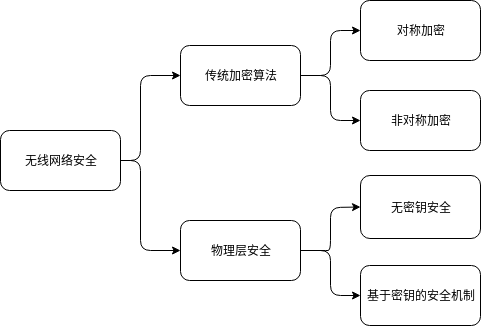
\includegraphics[width=0.9\textwidth]{images/wireless-network-security} 
    \caption{无线网络安全}
    \label{wirelss-network-security}
\end{figure}

本文研究无线信道密钥生成,即利用无线信道的随机性来生成密钥。和公钥体系利用数论问题保证安全性不同,无线密钥生成的安全性基于信息论。因为它基于无线信道的随机性\cite{ahlswede1993common}\cite{maurer1993secret},并且不需要借助其他用户的信息。以上所提及方法的优缺点列在表\ref{comparison-different-schemes}。

\begin{table}[]
    \centering
    \begin{tabular}{|p{80pt}|p{90pt}|p{70pt}|p{90pt}|p{90pt}|}
    % \begin{tabular}{|l|l|l|l|l|}
    \hline
    方法 & 描述 & 实现复杂度 & 优点 & 缺点 \\ \hline
    对称加密 & 合法通信双方用对称密钥加密数据 & 易实现 & 算法复杂度低 & 提前协商会话密钥;计算安全性 \\ \hline
    非对称加密 & 合法通信双方使用一对公私钥协商会话密钥 & 易实现 & 可用于协商会话密钥 & 计算安全性;依赖PKI;不适于低功耗设备 \\ \hline
    无密钥安全 & 合法通信双方通过设计编码和信道特性避免泄露信息 & 实现复杂 & 信息论安全;无需密钥的安全传输 & 依赖窃听者的CSI \\ \hline
    基于密钥的安全机制 & 合法通信双方利用信道的随机性生成密钥 & 易实现 & 信息论安全;轻量;无需第三方参与 & 受限于信道特性本身 \\ \hline
    \end{tabular}

    \caption{不同方法的比较
    \label{comparison-different-schemes}}
\end{table}

物理层安全的一个重点研究方面是密钥生成(SKG,Secret Key Generation)1993年Maurer和Ahlswede等人理论上提出密钥生成\cite{ahlswede1993common}\cite{maurer1993secret},研究一对观察共用随机源的合法通信者之间的密钥生成速率,并且该随机源对第三方窃听者透明。对于TDD模式的无线通信网络来说,由于上下行信道之间的短时互易性,合法通信双方可以使用无线信道衰落特性作为密钥生成的随机源。密钥生成的信道模型如图\ref{wireless-channel}所示。图\ref{wireless-channel}中Alice和Bob需要建立一个安全的加密通道,窃听者Eve与Alice相距d厘米,并监听了所有传输过程。Alice、Bob和Eve可以分别接收到信号$X^n = (X_1, ..., X_n)$,$Y^n = (Y_1, ..., Y_n), Z^n = (Z1, ..., Z_n)$。Alice和Bob在公共信道上交换消息s,Eve同样可以接收到消息s。对任何$\epsilon > 0$和足够大的$n$,如果存在$K^A = g_A(X^n, s)$和$K^B = g_B(Y^n, s)$使得密钥生成体系满足

\begin{eqnarray}
    Pr(K^A \neq K^B) < \epsilon \label{keyrate1} \\
    \frac{1}{n}I(K^A; s, Z^n) < \epsilon \label{keyrate2} \\
    \frac{1}{n}H(K^A) > R - \epsilon \label{keyrate3} \\
    \frac{1}{n}log[\mathcal{K}] < \frac{1}{n}H(K^A) + \epsilon \label{keyrate4}
\end{eqnarray}

那么式中R即可达密钥速率,其中$I(\cdot)$表示互信息,$\mathcal{K}$表示密钥key的字母表。公式\ref{keyrate1}表示Alice和Bob生成相同密钥的可能性;公式\ref{keyrate2}表示通过公共信道传输消息,不会泄露给窃听者Eve,从而保证密钥安全性;公式\ref{keyrate4}确保密钥是均匀分布。最大可达密钥速率可以用密钥容量定义,

\begin{equation}
    C_K = min[I(X;Y), I(X, Y|Z)]
\end{equation}

在具有丰富多径的无线通信环境中,信道响应具有空间唯一性,因此当上下行链路与上下行链路之间的距离超过半个波长,所有的上下行链路的信道响应之间是互相独立的\cite{jakes1994microwave}。所以第三方窃听者在半波长距离以外,难以分析出与合法通信信道完全精确的信道信息,其构成了基于信道随机性的无线信道密钥生成技术的基石\cite{aono2005wireless, badawy2015secret, koorapaty2000secure, sayeed2008secure, chorti2012helping, shehadeh2012towards, jana2009effectiveness, mathur2008radio, patwari2009high, croft2010robust, liu2014group, azimi2007robust, tope2001unconditionally, liu2014secret, badawy2016robust, zhang2016efficient, xi2014keep, liu2012exploiting, ye2010information, gungor2011secret}。根据密钥生成使用的信道特性,可以将目前研究分为三类,即空间角度\cite{aono2005wireless}\cite{badawy2015secret}、相位
\cite{koorapaty2000secure, sayeed2008secure, chorti2012helping, shehadeh2012towards}和幅度三种。由于离开角和到达角不同,角度的特征通常不互易,因此角度特征不够实用。基于幅度的密钥生成使用的信道特性有接收信号强度(Received Signal Strength,RSS)\cite{jana2009effectiveness, mathur2008radio, patwari2009high, croft2010robust, liu2014group}、信号包络\cite{azimi2007robust, tope2001unconditionally, liu2014secret, badawy2016robust, zhang2016efficient, xi2014keep, liu2012exploiting},幅度交叉
率(Level-Crossing Rate,LCR)\cite{ye2010information}和距离\cite{gungor2011secret}。因此基于相位和幅度的密钥生成方法更加值得研究和关注。

目前已经有一些研究工作实现上述理论。1995年第一个实际的密钥生成协议被提出\cite{hershey1995unconventional},之后陆续出现大量研究无线密钥生成的相关工作。\citet{WangSurvey}的第四章从信息论角度阐述了无线密钥生成。\citet{WangSurvey}将信道探测和量化合并为一个步骤来研究。\citet{zeng2015physical}介绍了密钥生成技术存在的机遇和挑战,但是未涉及到具体实现细节。\citet{ren2011secret}总结了一些密钥生成方法,比如基于接收信号强度(RSS)\cite{luo2016rss}和基于信道相位的方法\cite{wang2011fast}。

\section{研究内容和方法}

无线信道密钥生成协议通常包含四个步骤,信道探测、特征量化、信息调和以及隐私放大:

\begin{itemize}
    \item \textbf{信道探测}。信道探测是测量无线信道并提取无线信道特征的过程。通信双方互相收发导频信号,并从接收到的导频信号中提取信道特征。
    \item \textbf{特征量化}。特征量化是将无线信道特征通过预处理、归一化、量化等操作得到比特流的过程。由于提取的无线信道特征受到接收端增益等参数的影响,所以需要预处理、归一化等操作来使得双方探测的信道特征更加相近。之后,再量化成比特流。
    \item \textbf{信息调和}。信息调和是利用无线信道特征作为随机密钥源并结合合理可靠的交互协议生成会话密钥的过程。通信双方在探测信道之后,量化信道得到密钥,通过公共信道的交互协议去除密钥中的不一致比特,得到完全一致的会话密钥\cite{cachin1997linking}。
    \item \textbf{隐私放大}。隐私放大是进一步提高密钥随机性和可靠性、去除密钥中信道相关信息的过程。通过单向哈希函数等方法,可以移除密钥中隐藏的信道信息,进一步提高密钥的安全性\cite{cachin1997linking}。
\end{itemize}

本文基于GNURadio软件无线电开发平台,实现一种TDD/FDD下低时延宽带无线信道密钥生成系统。本文系统信道探测部分分为两种模式,一种TDD模式,另一种FDD模式,并研究两种模式下的信道互易性、密钥安全性等,设计TDD模式和FDD模式下低时延的会话密钥协商技术。无论是TDD还是FDD,其核心都是通信双方在相干时间内获取对端发射的导频信号,并从接收的导频信号中分析和提取信道特征。两种模式除了信道探测部分不同,其余三部分均比较相似。

TDD模式和FDD模式的主要不同点是收发导频信号的机制不同。TDD模式下,通信双方工作在同一频率,相干时间内,两个发送端发射的电磁波经管相同的信道衰落;FDD模型下通信双方工作在不同频率,收发导频信号几乎发生在同时。由于合法通信双方的通信信道在空间上唯一性,所以即便第三方窃听者监听到任意一方发送的导频信号,也无法分析出通信双方之间的CSI信息,以此保障密钥的安全。

无论是TDD模式还是FDD模式,通信双方提取出CSI之后的主要过程是相似的:量化、调和。由于无线信道的短时互易性,通信双方的CSI是相近的,在量化之后得到的比特流也是相似的,但是由于信道在探测时隙内发生变化以及周围环境中的干扰等各种因素,双方提取的密钥又是不完全一致的。因此需要进一步调和,去除不一致比特或者纠正错误比特。调和之后,通信双方会获取一致的比特流,为了进一步去除比特流中的信道信息,进行隐私放大得到最终的会话密钥。

GNURadio是软件无线电开发平台,被广泛应用于音频处理、移动通信、卫星追踪、GSM网络等计算机软件\cite{Blossom2004GNU},用户可以在GNURadio平台上设计、仿真以及部署高性能无线电的软件无线电系统。本文基于GNURadio软件无线电开发平台和USRP N210硬件,设计TDD/FDD下低时延宽带无线信道密钥生成系统,并验证生产环境下无线密钥生成技术的可靠性和安全性。

在现有关于无线密钥生成技术的研究中,无线密钥生成技术的理论和仿真居多,在实际生产环境中实现并验证的研究并不多见。本文基于GNURadio软件无线电平台,设计和开发了TDD/FDD模式下低延迟无线密钥生成系统,并在不同场景下采集数据,通过分析CSI的相关性、信道随机性、密钥随机性、信息泄露率等四种指标,充分验证无线密钥生成技术在实际环境中使用的安全性和可靠性。

\section{本文主要内容与章节安排}

本文主要研究无线信道密钥生成技术及其实际应用。文章先介绍了无线信道密钥生成技术的研究背景,并概述国内外无线信道密钥生成技术的研究现状,在现有研究基础上,基于GNURadio软件无线电平台,设计和开发TDD/FDD模式下低延迟无线密钥生成系统,并提出相应的系统性能评估指标,在多种场景下评估系统性能并分析系统优缺点。

\subsection{本文主要内容}

本文完成的主要工作包括:

\begin{itemize}
    \item(1)分析无线密钥生成技术的意义和背景,介绍无线密钥生成技术的国内外研究现状以及相关问题。
    \item(2)基于无线密钥生成技术的理论,设计完整的无线密钥生成技术方案,搭建TDD/FDD无线密钥生成系统。
    \item(3)基于TDD/FDD无线密钥生成系统,研究不同场景下无线密钥生成系统的安全性和可靠性,通过多次实验分析通信参与者CSI的相关性、无线信道随机性、密钥的随机程度、信息泄露量、密钥生成速率、系统的纠错性能,支撑无线密钥生成技术的实际应用意义。
\end{itemize}

\subsection{本文章节安排}

根据以上研究内容,本文分为六章,具体章节安排如下:

第一章分析当前无线通信网络中存在的问题,介绍无线密钥生成技术的应用背景和需求,概述当前国内外关于物理层安全的研究,最后给出本文研究内容和章节安排。

第二章阐述无线密钥生成系统的理论基础。首先介绍无线密钥生成技术的信道模型以及无线信道特性,之后详细介绍了无线密钥生成技术的主要步骤,最后给出无线密钥生成系统性能指标的理论依据。

第三章详细介绍了无线密钥生成系统的核心部分。首先介绍了系统中使用的导频信号格式以及检测方法,之后详细描述了导频信号收发机的设计方案以及每个组成模块。

第四章基于导频信号收发机设计完整的无线密钥生成系统,分别介绍了无线密钥生成系统的每个运行阶段。描述围绕导频信号收发机设计的时序逻辑,给出本文估计信道、量化特征、信息调和、隐私放大的具体算法。

第五章基于无线密钥生成系统,在实际环境中连续长时间采集数据,通过这些数据计算性能指标,评估不同场景下无线密钥生成系统的性能,比较TDD模式和FDD模式下性能指标的不同。

第六章总结本文主要工作,提出本文研究方法不足之处。

\chapter{无线密钥生成系统的理论基础}

本章节主要介绍无线密钥生成系统的理论基础。无线密钥生成系统的本质是利用无线信道的短时互易性、时空唯一性进行密钥生成的工作,在信道探测之后,量化生成的CSI,并进一步调和和隐私放大。另外本章介绍了系统生成密钥的评估标准,通过CSI相关性、信道随机性、密钥随机性和信息泄漏率等四个方面评估系统生成密钥的可靠性和安全性。

\section{无线信道特性}

\subsection{无线信道的短时互易性}

在TDD系统的上下行链路中,假设通信双方Alice和Bob以及窃听者Eve。在相干时间内,Alice和Bob互相发射的信号经过相同的信道衰落,因此由此估计出的信道具有互易性\cite{ye2010information}\cite{azimi2007robust}。

在图\ref{wireless-channel}中,Alice和Bob之间上下行链路的频率响应分别为$H_{ab}(t)$和$H_{ba}(t)$,相干时间内有$H_{ab}(t) = H_{ba}(t)$。假设在一次信道探测过程中,探测时隙为$\Delta t$,相干时间$\tau$内,Alice和Bob分别测量信道为$\tilde{H_{ba}(t)}$和$\tilde{H_{ab}(t)}$,当$ \Delta t < \tau $时有,

\begin{equation}
    H_{ba}(t) \approx H_{ab}(t + \Delta t)
\end{equation}

即双方探测的信道是近似相同的,因此通信双方可以通过利用无线信道的短时互易性来探测信道,进而结合其他协议生成相同的一致密钥。

同时,由于射频端的非线性特性、信道估计引入的误差、信道的时变性等因素\cite{guillaud2005practical},通信双方对信道的探测结果会有波动性差异:

\begin{itemize}
    \item 器件非线性。射频器件的非线性会导致I/Q路不平衡,如图\ref{iq_imbalance}所示,IQ不平衡会直接影响信号的发射和接收。在TDD系统中,收发两端的IQ不平衡会给上下行信道估计的互易性带来损失。
    \item 信道时变性。在相干时间内,无线信道具有短时互易性。但是由于无线信道的时变性,当双方探测信道的时隙超过信道相干时间,上下行信道估计结果会出现一定差异。
    \item 信道估计引入的误差。在基于导频的信号估计中,通过接收的导频信号和发射的导频信号做数学运算估计信道的频率响应,算法原理是通过最小化均方误差来估计信道,因此算法本身具有一定误差。
    \item 其他。另外,还有上下行链路的加性噪声也会对接收的信号有加性影响,不同频率子载波也会导致上行链路的差异等等。
\end{itemize}

\begin{figure}[htbp!]
    \centering 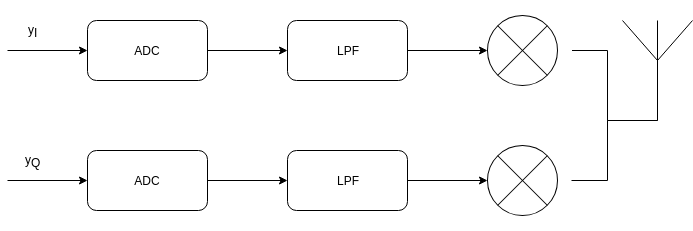
\includegraphics[width=0.9\textwidth]{images/iq_imbalance} 
    \caption{发射机存在的IO不平衡}
    \label{iq_imbalance}
\end{figure}


目前已经有相关工作研究如何对信道互易性的损失进行补偿,比如信道预测技术对信道互易性进行补偿,其原理是利用信道探测数据本身对未来时间的信道数据做出预测\cite{heidari2010adaptive}。另外基于信道互易性的MIMO预处理技术也可以一定程度上提高信道互易性,进而提高密钥一致性。针对IQ不平衡致使的信道互易性损失,可以估计系统中的不平衡参数,使相邻子载波的均方误差最小\cite{tubbax2005compensation}。

\subsection{无线信道的时空唯一性}

\begin{figure}[htbp!]
    \centering 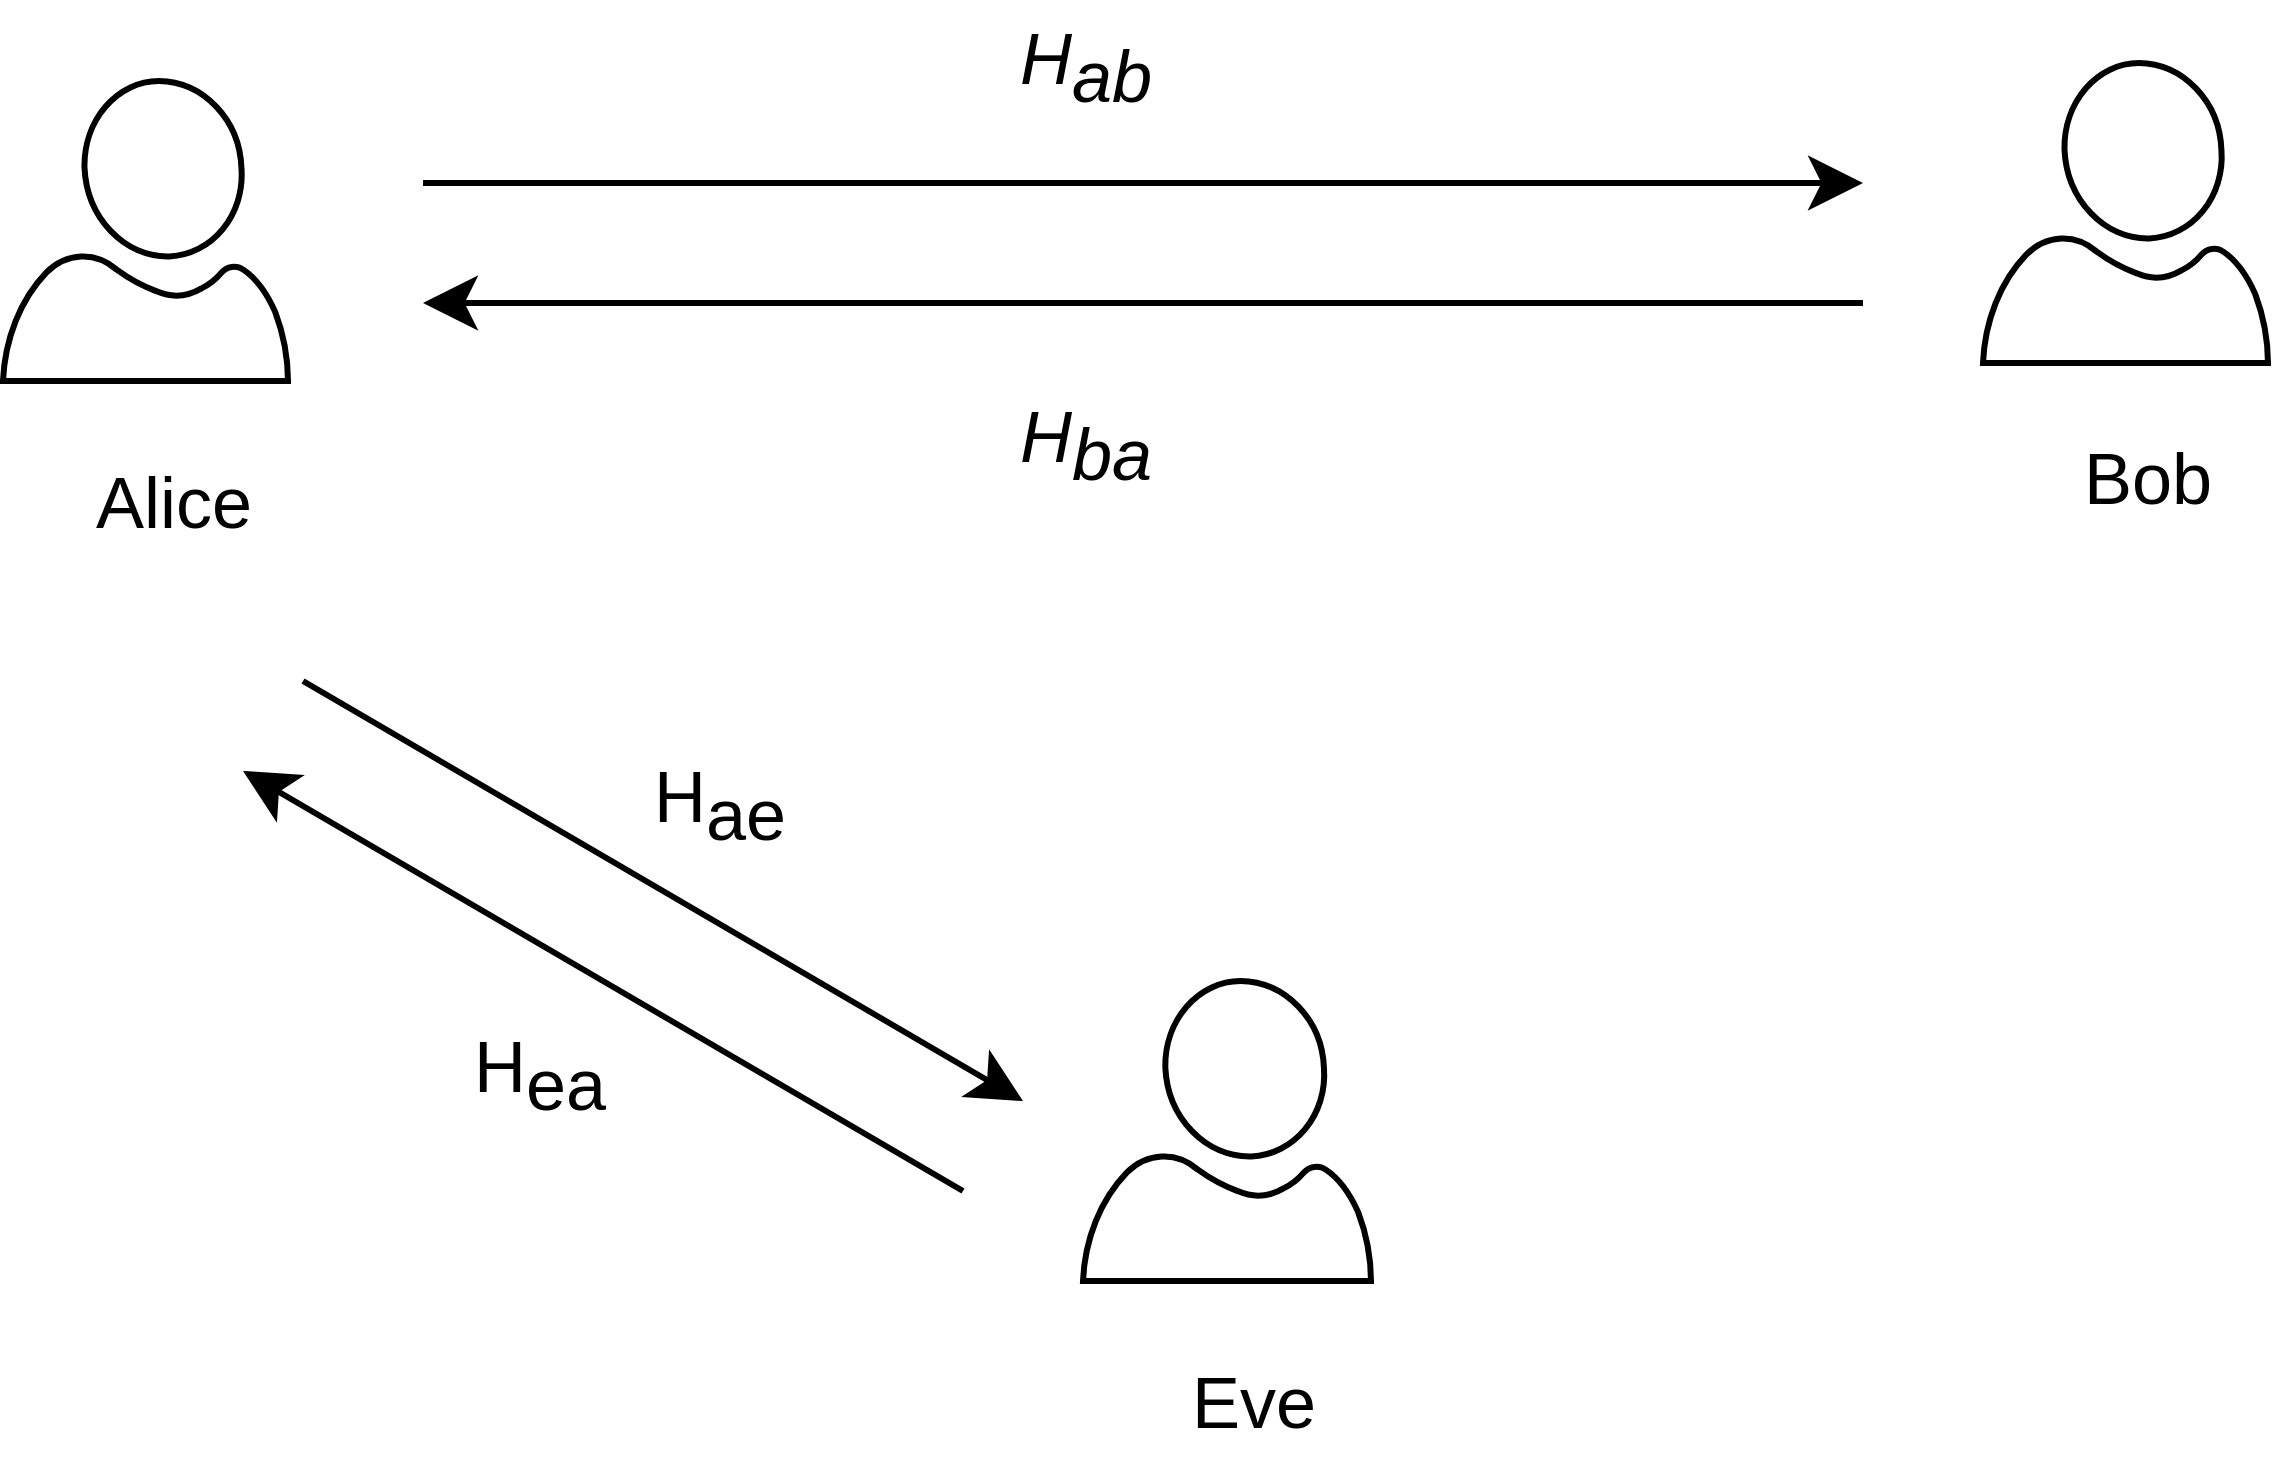
\includegraphics[width=0.9\textwidth]{images/channel} 
    \caption{无线通信信道}
    \label{wireless-channel}
\end{figure}

如图\ref{wireless-channel}所示,在某时刻t,通信双方Alice和Bob互相发射导频信号,在相干时间内,经管相同的多径信道衰落,对于窃听者Eve来说,无论是窃听来自Alice还是Bob的发射信号,其信道衰落都不同于Alice和Bob之间的信道衰落。在相干距离d(半波长)以外,Eve接收信号经历的多径衰落与Bob接收信号的多径衰落不再相关。除非攻击者在物理空间上靠近任意合法通信双方,否则无法分析出通信双方的CSI\cite{sasaoka2009secret}。

\subsection{无线信道的时变特性}

% 参考 3.1.1

信道衰落分为两类,大尺度衰落和小尺度衰落。大尺度衰落包括路径损耗和阴影损耗,在长距离传输(上百米)中,信号强度会发生变化。路径损耗指空间传播中电磁波的损耗,阴影损耗指在电磁波在传输过程中,受到遮挡物影响产生阴影效应,导致场强变化。通常用自由空间模型、Hata-Okumura,模型等来描述大尺度衰落。

小尺度衰落通常反应在短距离范围内信号幅值的变化中,通常符合瑞利分布、莱斯分布,小尺度衰落分为快衰落信道和慢衰落信道,快衰落信道又分为空间选择性快衰落信道、时间选择性快衰落信道、频率选择性快衰落信道。小尺度衰落反应无线信道的多径和时变,在无线通信中,通信双方之间信号经过的物理路径比较复杂,会收到多径的影响,可以将多径衰落信道建模成时变脉冲有限响应滤波器(FIR)\cite{liu2012exploiting},即,

\begin{equation}
    h(\tau, t) = \sum_{l = 1}^{N(t)} a_k(t) \sigma(\tau - \tau_k(t))
\end{equation}

其中,t时刻,多径分量个数为$N(t)$,$a_k(t)$表示t时刻第l条路径信号幅度,$\tau_k(t)$表示t时刻第l条路径的延迟。

在一次信道探测过程中,若探测间隙大于信道的相干时间,接收信号经历快衰落过程,即时间选择性衰落。若信号带宽大于信道的相干带宽,接收信号经历频率选择性衰落,接收信号会产生符号间干扰(ISI)。


\section{密钥生成流程}

本文基于无线信道密钥生成技术设计的系统主要分为四个阶段,信道探测、特征量化、信息调和,整体架构如图\ref{whole_structure}所示。其中,Alice和Bob是合法通信双方,Eve是第三方窃听者。信道探测阶段是无线信道传输导频信号,信息调和阶段是通过公共信道传输调和信息。

\begin{figure}[htbp!]
    \centering 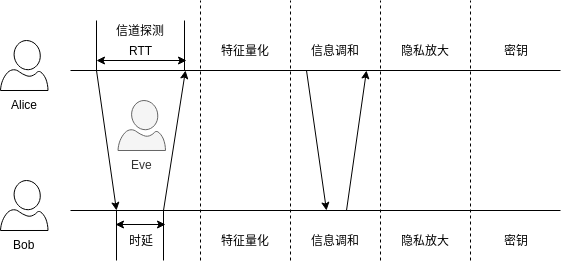
\includegraphics[width=0.9\textwidth]{images/whole_structure} 
    \caption{无线密钥生成流程的整体架构}
    \label{whole_structure}
\end{figure}

\subsection{信道探测}

在一个单入单出线性系统中,设脉冲响应函数为$g(k)$,根据维纳-霍夫方程的离散形式,发射信号$x(k))$和$y(k)$之间的相关函数为,

\begin{equation}
    R_{xy}(\tau)  = \sum_{j=0}^{\infty} g(j) R_x(\tau-j)\Delta t
\end{equation}

同时,M序列的自相关函数为,

\begin{equation} \label{m_self}
    R_m(\tau) = \left\{
  \begin{aligned}
  &1, &\tau = 0, N, 2N, ... \\
  &-\frac{1}{N}, &wherelse \\
  \end{aligned}
  \right.
\end{equation}

因此,当发射信号x(k)为M序列时,即$x(k) = m(k)$时,有,

\begin{equation}
    R_{ym}(k) = \sum_{j=0}^{N-1} \tilde{g}(j)R_m(k-j)\Delta t
\end{equation}
\begin{equation}
    R_{ym}(k) = \frac{(N+1)\Delta t}{N} \tilde{g}(k) - \frac{\Delta t}{N} \sum_{j=0}^{N-1} \tilde{g}(j)
\end{equation}
  
\begin{equation}\label{eq1}
    \tilde{g}(k) = \frac{N}{(N+1)\Delta t} [R_{ym}(k) + c]
\end{equation}

其中,

\begin{equation}
  R_{ym}(k) = \frac{1}{N}\sum_{j=0}^{N-1}m(j-k)y(j)
\end{equation}

工程上,

\begin{equation}
  c=-R_{ym}(N_P - 1)
\end{equation}
  
在TDD/FDD系统中,用户Alice和Bob互相发送导频信号帧$m(t)$作为导频信号。设$h_{ab}$代表Alice到Bob信道的频率响应,$h_{ba}$代表Bob到Alice信道的频率响应。那么,

Alice检测的时域信号为,

\begin{equation}
    y_{ba}(t) = m(t) * h_{ba}(t) + n_{ba}(t) 
\end{equation}

Bob检测的时域信号为,

\begin{equation}
    y_{ab}(t) = m(t) * h_{ab}(t) + n_{ba}(t)    
\end{equation}

因此Bob通过式(\ref{eq1})估计信道,

\begin{equation}
    \tilde{h}_{ab}(k) = a\sum_{j=0}^{N-1}m(j-k)y_{ab}(j)
\end{equation}
  
同理,Alice通过式(\ref{eq1})估计信道,
  
\begin{equation}
    \tilde{h}_{ba}(k) = a\sum_{j=0}^{N-1}m(j-k)y_{ba}(j)
\end{equation}
  
其中,a为常数,

\begin{equation}
    a = \frac{2-N_p}{(N + 1)\Delta t}
\end{equation}

\subsection{预处理}

在步骤信道探测中,通信双方分别通过导频信号估计探测时隙$\tau$内的脉冲响应$\tilde{h}_{ba}$和$\tilde{h}_{ab}$,并进行快速傅里叶变换得到信道频率响应$\tilde{H}_{ba}$和$\tilde{H}_{ab}$。由于在探测过程中,无线信道测量结果会受到环境噪声、射频器件的非线性等因素影响,因此通常会进一步预处理来提高信道的互易性和消除数据冗余。

\begin{equation}
    \tilde{H}_{ba} = Pre(FFT(\tilde{h}_{ba}))
\end{equation}
\begin{equation}
    \tilde{H}_{ab} = Pre(FFT(\tilde{h}_{ab}))
\end{equation}

其中,$Pre$表示预处理函数,$FFT$表示快速傅里叶变换。

\subsection{特征量化}

目前有多种量化策略,常用的有单门限量化、多门限量化、自适应门限量化等。

文献\citet{aono2005wireless}采用如图\ref{single_quantization}所示的单门限量化,量化阈值取RSSI(Radio Signal Strength Indicator)平均值,可以带来比较高的密钥一致率,但是测量值在阈值附近时容易量化错误,并且由于量化精度不高,在信道变化缓慢时,生成密钥容易出现大量连续0比特和1比特长串。

\begin{figure}[htbp!]
    \centering 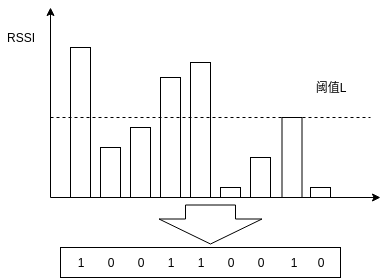
\includegraphics[width=0.9\textwidth]{images/single_quantization} 
    \caption{单门限量化}
    \label{single_quantization}
\end{figure}

文献\citet{mathur2008radio}采用如图\ref{two_quantization}所示双门限量化,将门限$L^+$和$L^-$之间的值舍弃,将$L^+$以上的值量化为1,将$L^-$以下的值量化为0,通信双方会在公共信道上交互传输未舍弃比特位的索引信息,因此第三方窃听者只有可能得知哪些比特被使用而无法得知被量化成0还是1,但是会降低密钥生成速率。

\begin{figure}[htbp!]
    \centering 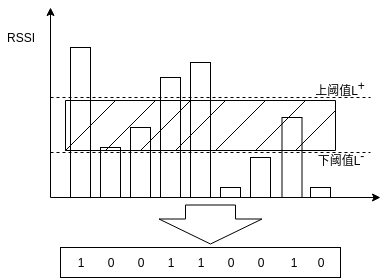
\includegraphics[width=0.9\textwidth]{images/two_quantization} 
    \caption{双门限量化}
    \label{two_quantization}
\end{figure}

文献\citet{patwari2009high}通过多次测量表明双门限量化每次会丢失5\%至27\%的比特数,并提出多比特自适应量化方法。文献\citet{yasukawa2008secret}使用多级量化,先将RSSI根据大小排序,然后分割成等间隔的$N = 2^m$块,m是量化比特数,并且通常$N \leq log_2^{maxValue}$,这样每个量化阶值的出现率是相同的。

通常多比特量化之后,会进一步编码成对应阶数格雷码。格雷码的特性是,相邻位置的格雷码只有一个位置的比特不同,因此使用格雷码可以提高通信双方的密钥一致率。无论是上述哪种量化方法,都避免不了密钥生成率和密钥一致性之间的矛盾。量化阶数越高,量化比特数越多,密钥生成率越高,但误差影响较大,密钥一致率降低;量化阶数越低,量化比特数越少,密钥一致率越高,但是密钥生成速率越低。

本文使用均匀量化的方法。在一次密钥生成过程中,Alice和Bob分别探测信道、预处理得到CSI。先对CSI降采样,以降低密钥泄漏率\cite{linning2019investigation}。同时,量化可以降低噪声的影响\cite{wang2015survey}。设量化时CSI最大值为$m_{max}$,量化阶数为R,量化前的值为m,量化后的值为q,将CSI归一化后按照式\ref{quantization_formula}均匀量化,得到离散的采样值,采样值对应比特数即量化阶数,本文量化阶数为3。密钥的生成速率与量化阶数成正比,通信双方的密钥一致率与量化阶数成反比。因此可以根据信噪比去调整量化阶数以得到较为均衡的密钥生成速率与一致率。量化之后的采样值需要进一步格雷编码降低密钥的不一致率。然后进行8b10b编码,过程如图\ref{quantization}所示。

\begin{equation} \label{quantization_formula}
    q = \frac{2^R * m}{m_{max}}
\end{equation}

\begin{figure}
    \centering
    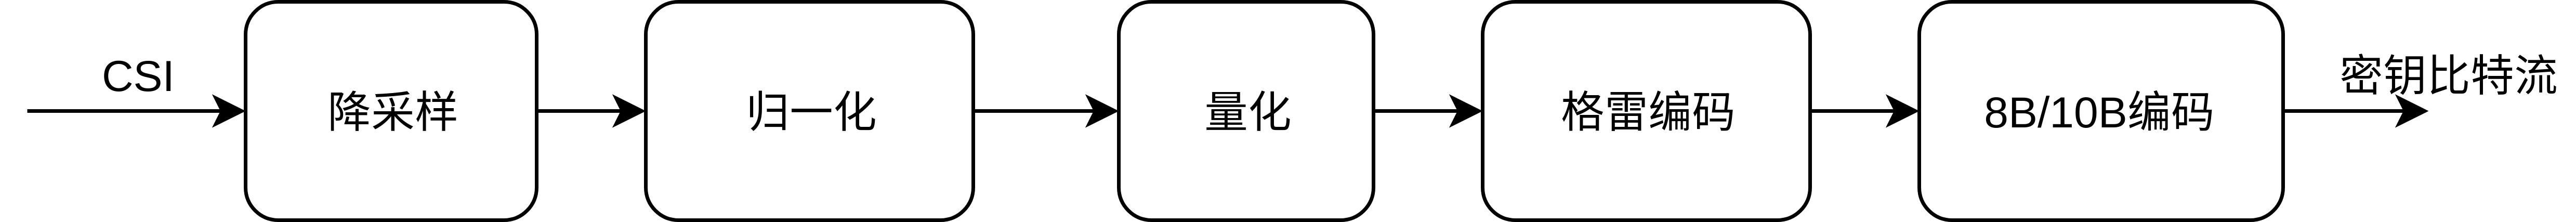
\includegraphics[width=0.9\textwidth]{images/quantization}
    \caption{量化}{} % Quantization.
    \label{quantization}
\end{figure}

\subsection{信息调和}

信息调和是在公共信道对不完全一致的密钥信息协商。由于短时信道互易性,所以通信双方分别通过上述步骤提取出的密钥是近似的,但是由于信道在探测的时隙内发生变化、环境中的干扰以及硬件指纹等各种因素,双方提取出的密钥又是不完全一致的。因此需要进一步调和。

信息调和通常基于Caseade协议\cite{Kitano2007A}或者纠错编码,比如 Turbo 码,BCD 码,LDPC 码等\cite{peng2018securing}。本文使用两种方式调和生成密钥。假设通信双方Alice和Bob,量化之后提取的比特字符串为$key1$和$key2$。

如果通过CRC校验码去除不一致比特,那么Alice将比特字符串$key1$分组并计算CRC校验码,将冗余部分码字发送给Bob。Bob进行同样分组,并根据Alice发送过来的冗余部分码字去除不一致的组。Bob再将检验结果回发给Alice,Alice根据校验结果去除不一致的组。最终双方可以得到一致的会话密钥。使用CRC校验码的调和过程如图\ref{crc}所示。

\begin{figure}
    \centering
    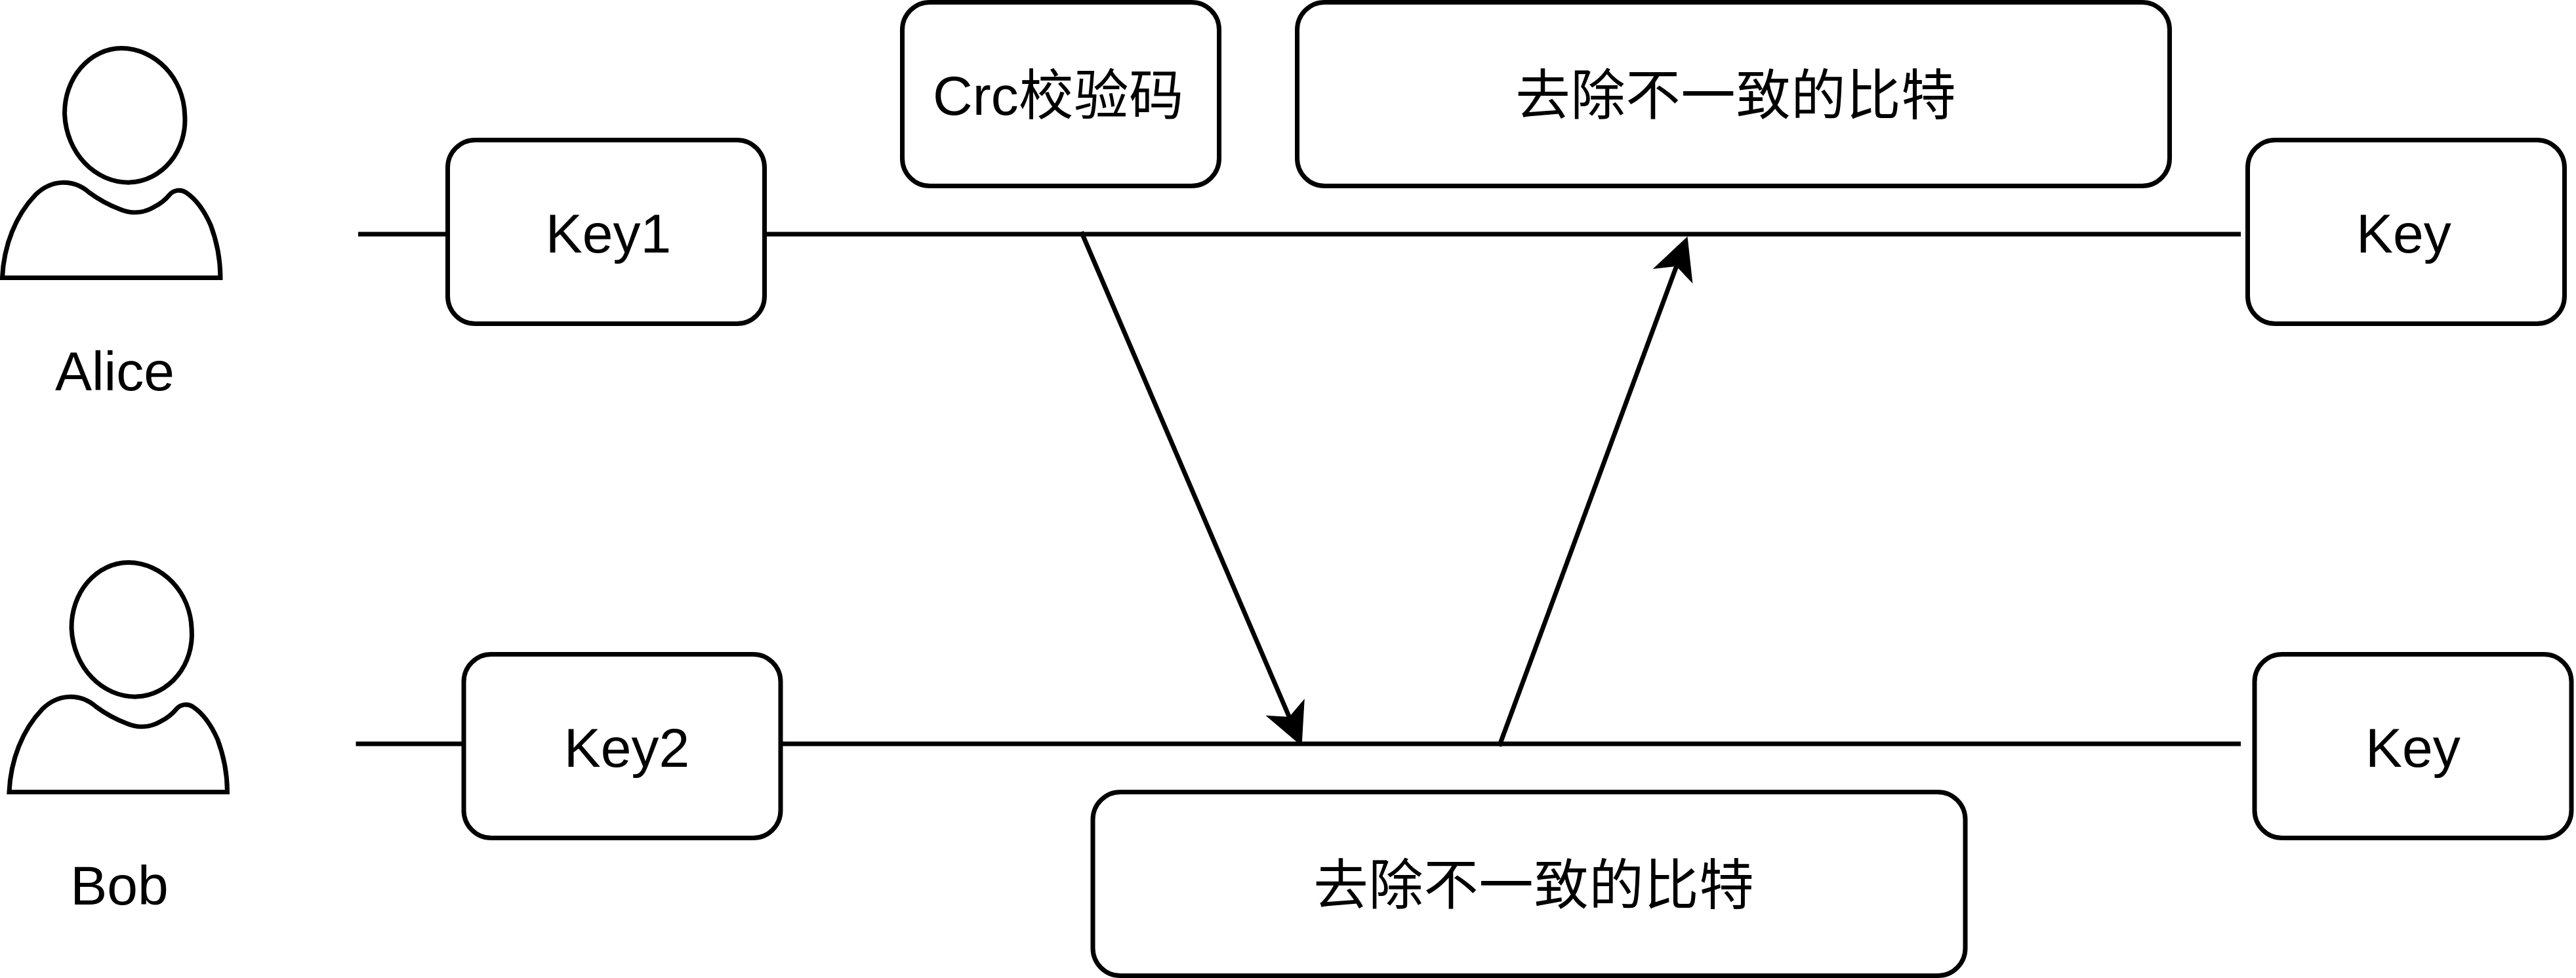
\includegraphics[width=0.9\textwidth]{images/crc}
    \caption{信息调和}{} % Crc Reconciliation
    \label{crc}
\end{figure}

% todo 纠错解码着一块还可以写的更加详细一点
除了通过CRC校验码去除不一致比特,Alice先将会话密钥进行纠错编码,再和key1异或,然后发送给Bob,Bob再次和key2异或,之后通过纠错解码器纠正错误比特位得到会话密钥key'。使用纠错码的过程如图\ref{error_correcting_code}所示。

\begin{figure}
    \centering
    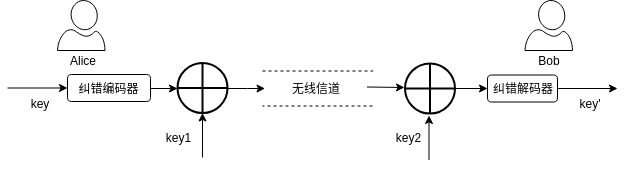
\includegraphics[width=0.9\textwidth]{images/error_correcting_code}
    \caption{纠错码}{} % Crc Reconciliation
    \label{error_correcting_code}
\end{figure}

% TODO
\subsection{隐私放大}

由于信道探测阶段和信息调和阶段,通信双方之间交互的中间信息对外界全部透明,中间信息中可能分析出密钥,因此为了防止密钥信息被泄露,所以需要进一步隐私放大。隐私放大是允许双方从窃听者拥有部分信息的公共随机变量中提取密钥的过程。双方一般对窃听者的信息一无所知,只知道它满足一定的约束条件。隐私放大使得密钥协商成为可能,在密码学领域有着广泛应用\cite{vernam1926cipher}。

假设Alice和Bob拥有变量W(n比特),窃听则Eve从变量W中窃听到变量V(t比特,t < n且比特位随机),并且满足约束$ I(W;V) \leq t $,那么Alice和Bob可以仍然协商出Eve无法得知的$n-t$比特的密钥\cite{bennett1988privacy}。通常可以使用Hash函数来完成隐私放大\cite{wegman1981new},其将任意长度的字符串映射到一个固定长度的字符串。

\section{无线信道密钥的评估标准}

本文为评估无线密钥生成系统性能,通过CSI相关性、信道随机性、密钥随机性和信息泄漏率等四个方面评估系统生成密钥的可靠性和安全性。

\subsection{CSI相关性}

本文通过皮尔逊相关系数计算CSI相关性,假设通信系统中,合法通信双方Alice和Bob信道探测结果为$\tilde{H}_{ba}$和$\tilde{H}_{ab}$,窃听者Eve探测结果为$\tilde{H}_{ae}$。

那么Alice和Bob之间CSI相关性为,

\begin{equation}\label{equation_corr_ab}
    Reprocity_{ab, ba} = \frac{E[(\tilde{H}_{ab}-\mu_{\tilde{H}_{ab}})(\tilde{H}_{ba}-\mu_{\tilde{H}_{ba}})]}{\sigma_{\tilde{H}_{ab}}\sigma_{\tilde{H}_{ba}}}
\end{equation}

为研究Eve窃听的CSI结果与合法信道的CSI结果的差异,计算Eve的CSI和Alice的CSI相关性,

\begin{equation}\label{equation_corr_ae}
    Reprocity_{ab, ae} = \frac{E[(\tilde{H}_{ab}-\mu_{\tilde{H}_{ab}})(\tilde{H}_{ae}-\mu_{\tilde{H}_{ae}})]}{\sigma_{\tilde{H}_{ab}}\sigma_{\tilde{H}_{ae}}}
\end{equation}

其中,$\sigma_{\{.\}}$表示标准差,$E\{\cdot\}$表示期望。

理论上,在相干距离之外,

\begin{equation}
    Reprocity_{ab, ae} < Reprocity_{ab, ba}
\end{equation}

$Reprocity_{ab, ba}$越大表明合法通信双方信道互易性越好,CSI相关性越高,密钥一致率越高。$Reprocity_{ab, ba}$较低的原因可能是通信双方硬件指纹差异、信道环境糟糕等,可以使用一些预处理算法弥补互易性的损失。

$Reprocity_{ab, ae}$越小表明第三方可以窃听的信息越少,CSI相关性越低,密钥泄露更少。在相干距离(通常是半波长)以外,由于导频信号经过不同的信道衰落,因此Eve估计得到的CSI与合法信道的CSI相关性较低。在相干距离以内,由于物理距离上接近,Eve估计的CSI相关性较高,但是在实际环境中,窃听者无法如此靠近合法通信参与者。

\subsection{信息泄露率}

本文设计的密钥生成系统中,在信道探测、信息调和阶段,对第三方来说是完全透明的\cite{sahin2016secure}。设Alice、Bob和Eve对信道探测为$H_A$、$H_B$和$H_E$。则A和B之间信道的互信息为,

\begin{equation}
    I_k = I(H_A; H_B) = log_2^{\frac{\left|R_{AA}\right|\left|R_{BB}\right|}{\left|R_{AB}\right|}}
\end{equation}

其中, $\left|R_{xy}\right| = E\{H_x H_y^H\}$表示协方差系数。

存在eve时,alice和bob之间的互信息量为, 

\begin{equation}
  I_{sk} = I(H_A; H_B | H_E) = log_2^{\frac{\left|R_{AE}\right|\left|R_{BE}\right|}{\left|R_{EE}\right|\left|R_{ABE}\right|}}
\end{equation}

通过$I_{sk}$与$I_k$的比例来评估信息未泄露的比率,

\begin{equation} \label{safe_rate_equation}
  \eta = I_{sk} / I_k
\end{equation}

\subsection{随机性评估}

本文既评估了系统运行过程中的CSI随机性,也测试了生成密钥的随机性。

\subsubsection{CSI随机性}

CSI的随机性既有时域的变化,也有频域的变化。为了衡量CSI的随机性,本文采集了不同场景下的多组CSI,计算多组CSI的图像熵,用来衡量CSI的随机性。

使用二维快速傅里叶变换(2d-fft)的图像熵来表征信道的随机性。设计算得到的多组CSI归一化之后为矩阵$C_{MxN}$,M为CSI长度,N为采集的CSI组数。$C(x, y)$表示第i行第j列的值,那么对其做2d-fft计算,其2d-fft的矩阵为,

\begin{equation}
  F(u, v) = \frac{1}{MN}\sum_{x=0}^{M-1}\sum_{y=0}^{N-1} C(x,y) e^{-j2\pi(\frac{xu}{M}+\frac{yv}{N})}
\end{equation}


为了缩小差距,将$F$取In函数得到$L$,

\begin{equation}
  L(u, v) = log_e^{F(u, v)}
\end{equation}

再归一化到[0, 1]范围内得到,

\begin{equation}
  I(u, v) = \frac{L(u, v) - min{L}}{max(L) - min(L)}
\end{equation}

将[0, 1]区间分割成256等份,统计I(u, v)在各个区间的概率,计算I(u, v)的熵,

\begin{equation} \label{entropy_fft2d_equation}
  H(u, v) = -\sum_{i=1}^{256} p_i log_2^{p_i}
\end{equation}

\subsubsection{密钥随机性}

本文使用NIST(National Institute of Standards and Technology,NIST)随机性测试来评估密钥的随机性\cite{bassham2010statistical}。NIST随机性测试通过多个维度测试密钥的随机性\cite{zaman2012review}。NIST官网包含了16项统计测试,每项测试会对给定比特序列做在随机性假设下的卡方检验,其将$\chi^2$值转换为随机性概率,即程序中的P值,表示随机性的可能性大小。表\ref{NIST-schemes}为NIST随机性测试的15项测试手段。如果P值大于0.01,则表示比特序列是随机的。

% 参考

\begin{table}[]
    \centering
    \begin{tabular}{p{70pt}p{70pt}p{200pt}p{100pt}}
    \hline
    方法 & 参数要求 & 原理 & 不通过原因 \\ \hline
    频数检验 & N $\geq$ 100bits & 序列中1和0数目是否相近 & 说明1和0数目相差过多  \\ \hline
    块内频数检验 & N $\geq$ 100bits 子块 M > 0.01N & M位子块中1的个数是否接近m/2 & 至少某一个子块0、1比例不均衡 \\ \hline
    游程检验 & N $\geq$ 100bits 设定$\tau = \frac{2}{\sqrt{n}}$,用于判定是否频数检验 & 检验不同长度的游程总数是否符合随机序列的期望值 & 说明游程综述过大或者过小,即,序列中元素变化过快或者过慢  \\ \hline
    块内最长游程检验 &  & 检验序列中各个等长子序列中最长1游程的长度是否符合随机序列的期望值 & 检验序列中有太多的(成簇的)1 \\ \hline
    二元矩阵秩检验 & N $\geq$ 38MQ,行列M=Q=32 & 由检验序列的给定长度子序列构成序列,检验构造矩阵行或列之间的线性独立性 & 秩分布与相应的随机序列有一个大的偏离 \\ \hline
    离散傅里叶变换检测 & N $\geq$ 1000 & 使用频谱方法检验序列进行傅里叶变换后的尖峰高度是否超过某个门限值 & 太多傅里叶变换的尖峰高度超过门限值 \\ \hline
    非重叠子模块检验 & $ N \geq 10^6$  m={9, 10} & 使用一个m-bit窗口来搜索一个特定的m-bit模式,检验设置好的目标数据串的发生次数 & 存在无规则发布的模块 \\ \hline
    重叠子序列检验 & $N \geq 10^6$ m={9, 10} & 检测提前设置好的目标数据串发生的数目与非重叠子模块相似,不同之处在于发现目标模块后,窗口仅向后移动一位 & 在太多的目标数据串存在 \\ \hline
    Maurer通用统计检验 & & 检验序列是否可被无损压缩 & 序列可大幅度的被压缩 \\ \hline
    % Lempel-Ziv压缩检验 & $N \geq 10^6$ & 检验序列能够被压缩到什么程度 & 序列可以被很大程度压缩,说明非随机 \\ \hline % 在最新版本中已经被去除
    线性复杂度检验 & $N \geq 10^6$ & 检验各等长的子序列的线性复杂度是否符合随机序列期望值 & 子序列线性复杂度分布不规则 \\ \hline
    序列检验 & $ m < [log_2^N] - 2$ & 检验序列中m位可重叠子序列的每一种模式个数是否接近,对随机序列来说,m位可重叠子序列的每一种模式出现的概率应该相等。m=1时即1 & 序列中长度为m的可重叠子序列模式分布不均匀 \\ \hline
    近似熵检验 & $ m < [log_2^N] - 2$ & 看整个序列中所有可能的重叠的m-bit模式的频率,目的是将两相邻长度(m和m+1)的重叠子块的频数与随机情况下预期的频数相比较 & 序列有较强的规律性 \\ \hline
    累加和检验 & $N \geq 100bits$ & 最大累加与随机序列中具有的最大偏移相比较,应该接近0 & 说明序列早期或者晚期有过多1或者1 \\ \hline
    随机游动检测 & $N \geq 10^6$ & 看一个累加和随机游动中具有K个节点的循环个数 & 与预期背离 \\ \hline
    随机游动状态频数检验 & $N \geq 10^6 $ & 看累加和随机游动中经历的特殊状态的总数。检验目的即:判定随机游动中实际经历多个状态的值和预期值之间的偏离程度 \\ \hline

    \end{tabular}
    \caption{NIST测试
    \label{NIST-schemes}}
\end{table}

\subsection{密钥不一致率和密钥生成速率}

密钥不一致率(KDR,Key Disagreement Rate)指在调和之前,通信双方生成密钥的不一致比特占比。高KDR通常表示密钥生成协议的效率较低,甚至可能由于KDR较高导致错误比特数超过纠错码的纠错极限。基于RSS的密钥生成方法的KDR通常由无线信道的多径和时变决定\cite{jana2009effectiveness}。通过多天线可以提高KDR,因为多天线可以提供更多的互信息。在一个低信噪比(SNR)的环境中,由于信道估计的误差更大,所以KDR更低。

密钥生成速率(KGR,Key Generate Rate)可以用于表示系统生成密钥的效率,即平均每秒或者每次信道测量最终可以生成的密钥比特数。KGR越高,通信双方可以在短时间内建立会话密钥,达到较高通信效率。基于RSS的密钥生成方法通常KGR非常低,因为该方法需要平衡KGR、KDR。为了减少KDR,通常不得不将连续多个值当做一个比特处理,此外该方法的KGR收到瑞利衰减信道的幅度交叉率限制(level-crossing rate)。虽然过采样可以带来更高的信道相关性,但是却会导致密钥随机性降低\cite{mathur2008radio}。多天线系统可以带来几乎四倍于普通方法的密钥生成率\cite{zeng2010exploiting}。

\section{本章小结}

本章主要介绍无线密钥生成系统的理论基础,首先介绍无线信道的特征对无线信道密钥生成的影响,无线信道的短时互易性是无线密钥生成技术的基石,无线信道的时空唯一性决定第三方窃听信息的困难程度,无线信道的时变性会给无线密钥生成技术带来信道互易性上的损失。

之后详细阐述密钥生成流程的主要阶段,包括信道探测、预处理、特征量化、信息调和等无线信道密钥生成步骤的具体理论。信道探测用于获取CSI,预处理为了提高信道互易性,特征量化用于提取密钥比特流,信息调和步骤中协商生成一致的密钥比特流。

最后提出密钥生成系统性能的评估指标,包括CSI相关性、信息泄露率、CSI随机性、密钥随机性、密钥生成率、密钥不一致率等指标,用于衡量无线密钥生成系统的可靠性和安全性,CSI相关性和信息泄漏率表征第三方窃听信息的难度,CSI随机性和密钥随机性分别评估信道的随机性和密钥的随机性,密钥生成率表示系统生成密钥的效率,密钥不一致率表示通信双方调和前密钥的一致性。

\chapter{导频信号收发机设计}

在TDD通信系统中,考虑一对合法用户Alice和Bob在多径衰落信道工作,通信双方互相发送已知导频信号。在想干时间$\tau$内,通信双方发送的信号经过相同信道衰落到达对方。接收方由接收的导频信号与已知导频信号估计$\tau$这段时间内的信道。


% TODO 是否要加入纠错码这一块的详细设计和解释
\section{导频信号}

\subsection{粗同步}
通信双方Alice和Bob均需要发送导频信号用于在通信过程中估计信道所用。在信道探测步骤中,为了可以更快的检测出指定信号,本文在导频信号首尾分别添加一段正弦波,如果检测到指定长度信号的首尾两端出现指定频率的正弦波,则说明该段信号是指定导频信号,将其存储供信道估计使用。

本文将以上步骤称为粗同步。设Alice发射导频信号为$Frame_a$,长度为$L_a$,$Frame_a$中首尾两端正弦波频率为$F_a$,检测阈值为$R_a$,fft长度为$L_d$,正弦波长度为$L_{sine_a}$。设Bob发射导频信号为$Frame_b$,长度为$L_b$,$Frame_b$中首尾两端正弦波频率为$F_b$,检测阈值为$R_b$,fft长度为$L_d$,正弦波长度为$L_{sine_b}$。GNURadio中处理数据的形式是高速实时数据流的形式,以Bob为例,接收数据流$S_a$对每段数据流输入,均会有数据流输出,本文对每L个长度的复数点做fft得到频域响应$H_{detect_a}$,并检查$ L_d - L_d / F_a $处幅值是否大于阈值$R_a$。即,在数据流$S_a$的位置i处计算,

\begin{equation}
    H_{detect_a} = FFT(S_a[i, i+L_d])
\end{equation}

若,

\begin{equation}
    H_{detect_a}[L_d - L_d / F_a] \geq R_a 
\end{equation}

则$S_a[i, i+L_d]$这段信号是指定$F_a$频率正弦波,说明这段信号前后存在需要检测的导频信号。为了确定导频信号在输入信号中的具体位置,需要判断距离相隔$L_a - L_{sine_a}$两个位置是否同时存在指定$F_a$频率的正弦波,如果这两个位置同时存在指定$F_a$频率的正弦波,那么这两个位置之间即需要检测的Alice发射的导频信号。即,在数据流$S_a$的位置$i$处和位置$i+L_a-L_{sine_a}$处计算,若,

\begin{equation}
    FFT(S_a[i, i+L_d])[L_d - L_d / F_a] \geq R_a 
\end{equation}

\begin{equation}
    FFT(S_a[i+L_a-L_{sine_a}, i+L_a-L_{sine_a}+L_d])[L_d - L_d / F_a] \geq R_a 
\end{equation}

那么,数据流$S_a$的位置$i$处和位置$i+L_a-L_{sine_a}$之间的数据即Bob需要检测得到的、Alice发射的导频信号,将这之间的信号保存下来。对于Alice来说,同理。

粗同步步骤出现在GNURadio检波程序中,相对于传统的相关检波,其时间复杂度更低。在检测过程中,会对每$L$长度的信号段做阈值检测,当出现前后两端正弦波并且间隔满足指定导频信号的要求时,即检测到导频信号,其过程如图\ref{detect_wave_algm}所示。

\begin{figure}
    \centering
    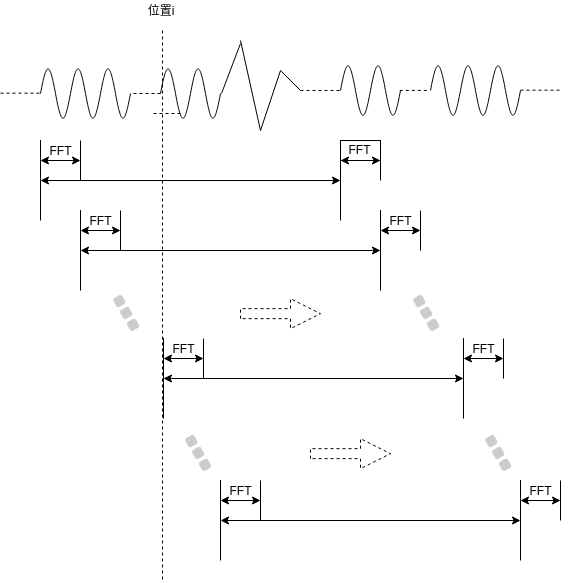
\includegraphics[width=0.9\textwidth]{images/detect_wave_algm}
    \caption{粗同步检波}{} % Crc Reconciliation
    \label{detect_wave_algm}
\end{figure}


\subsection{精同步}

在粗同步中,检波模块将检测到的导频信号转存到硬盘中,转存到硬盘的导频信号首尾两端是不完整的正弦波,首尾两端正弦波长度之和应该是$L_{sine_a}$,但是首部和尾部分别多长无法得知,因此需要进一步精确同步。

本文使用伪随机性序列(PN序列)作为精确同步和信道估计所用序列,由于m序列是PN序列中的一种,并且具有良好的自相关特性,所以本文使用m序列作为导频信号的主体部分。为了消除符号间干扰(Inter-Symbol-Interference,ISI)和载波间干扰(Inter-Carrier-Interference,ICI),在m序列后面添加循环前缀(Cyclic Prefix, CP)充当保护间隔,CP指的是将m序列的前面一部分复制到后段。

% TODO 加入仿真和实际测量中m序列自相关的图片
因为精同步发生在导频信号检测并转存之后,对实时性要求不高,因此本文利用m序列的自相关特性来精确切割导频信号。m序列的自相关函数是公式(\ref{m_self})所示周期性的二值函数,m序列的自相关函数时域上与冲激函数相近,在完全重合的周期点会出现波峰,并且随着m序列周期增加,m序列的随机性越好。设通信方转存的导频信号为$Rx$,包含的m序列理想情况为$m$,长度为$L_m$,第一段正弦波的完整长度为$L_{sine}$,那么可以遍历导频信号的起始一段,通过与已知原始m序列共轭相乘相加,求出波峰$Peak$并保存波峰位置i,

\begin{equation}
    Peak = max\{\frac{\sum_{k = i}^{L_m} \bar{m(k})\times Rx(i + k)}{L_m}) \}, i \in \{1, .., L_m + L_{sine}\}
\end{equation}

其中$\bar{\dot}$为取共轭。波峰$Peak$处对应的位置$i$就是精同步的结果,即m序列的起始位置,计算出m序列起始的精确位置,便可以进一步通过m序列或者其他数据段进行信道估计步骤。

图\ref{practical_pilot_m_seq}为系统转存的实际导频信号,其中包含第一段检波所用正弦波,以及m序列。通信方已知m序列原始信号如图\ref{m_seq}所示。图\ref{m_corr_practical}展示在实际系统中,转存信号中与已知m序列做相关的结果,其中根据波峰位置可以精确定位导频信号中m序列的起始位置。

\begin{figure}
    \centering
    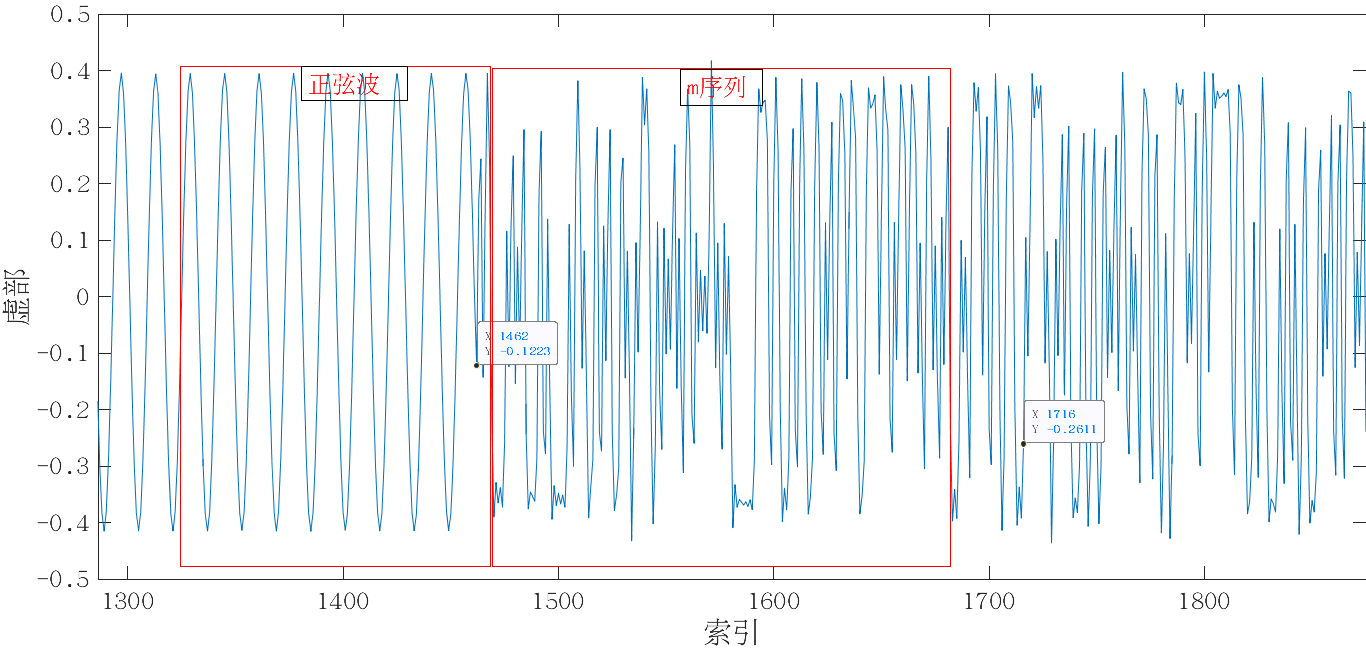
\includegraphics[width=0.9\textwidth]{images/practical_pilot_m_seq}
    \caption{实际导频信号中的m序列}{} 
    \label{practical_pilot_m_seq}
\end{figure}

\begin{figure}
    \centering
    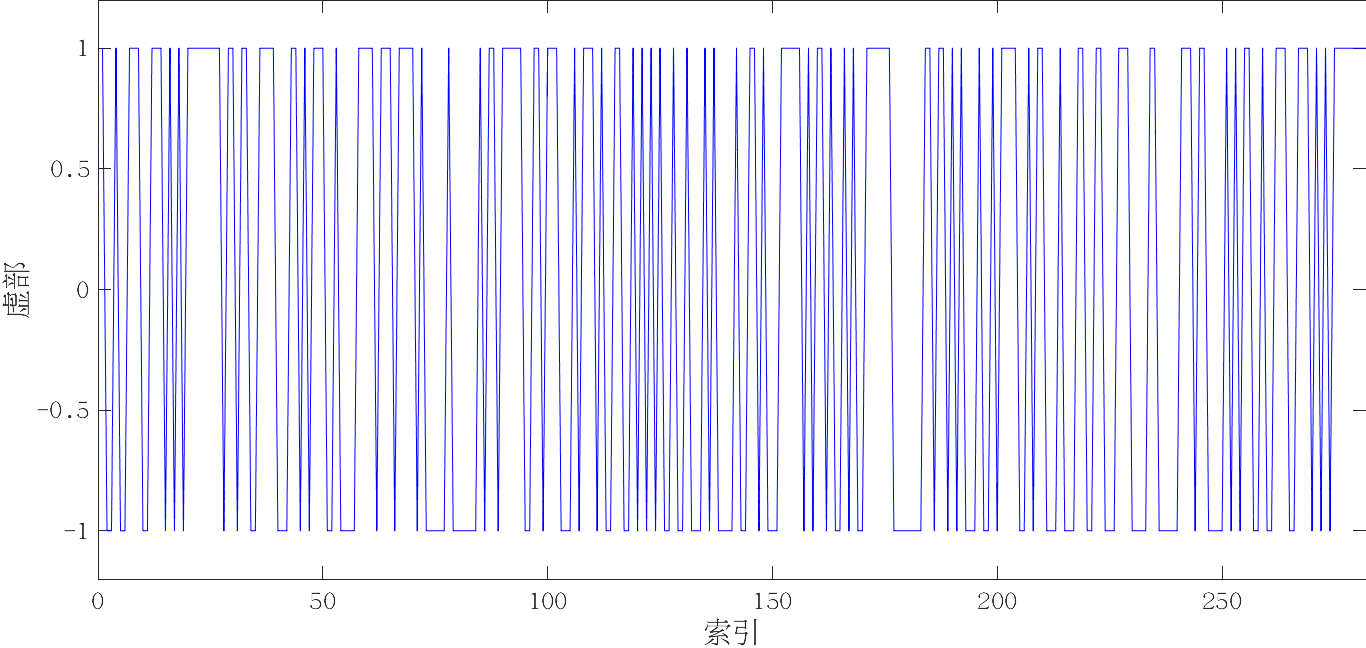
\includegraphics[width=0.9\textwidth]{images/m_seq}
    \caption{理想情况下的m序列}{} 
    \label{m_seq}
\end{figure}

\begin{figure}
    \centering
    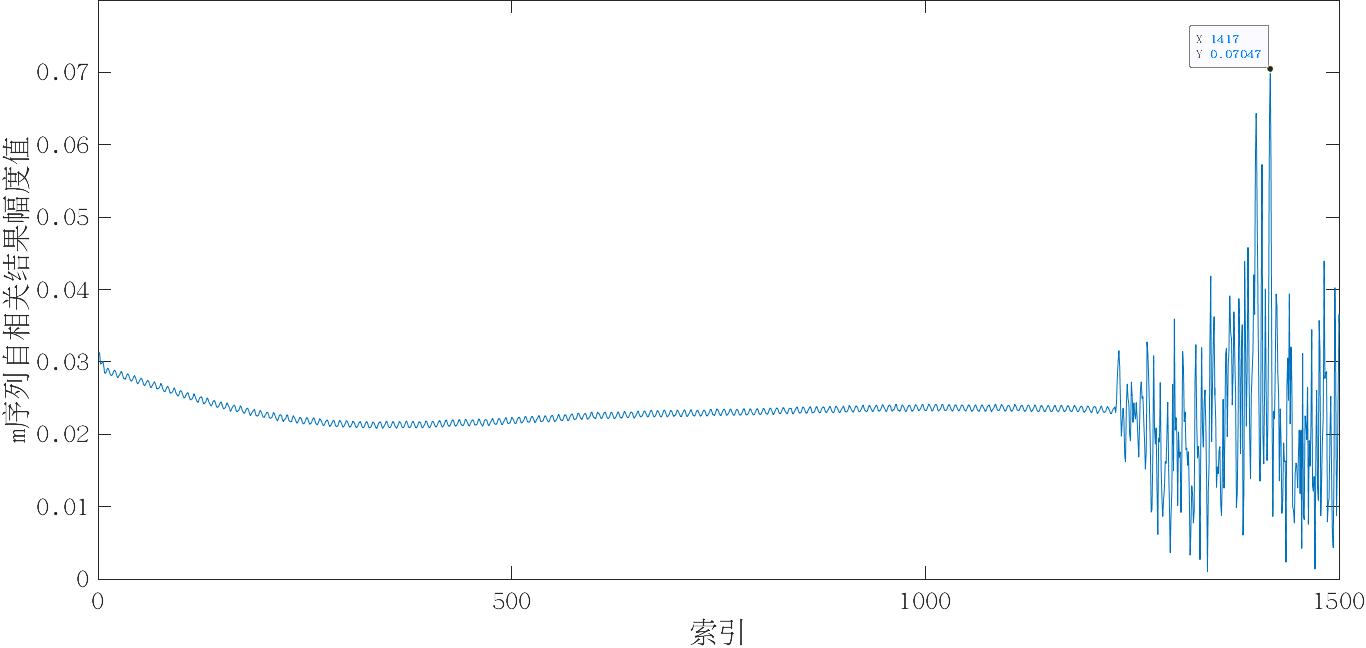
\includegraphics[width=0.9\textwidth]{images/m_corr_practical}
    \caption{理想和实际中m序列自相关}{} % Crc Reconciliation
    \label{m_corr_practical}
\end{figure}

\section{基于导频信号TDD收发系统设计}

本节阐述基于导频信号的TDD收发系统设计,从理论以及实现的角度详细介绍系统的构造。导频收发机是基于GNURadio搭建的,数据采集由USRP部分负责,USRP射频前端将数据转换到基带信号,并送入通用计算机中处理数据,实际上检波部分运行在计算机内,USRP将基带数据通过网口送入计算机内,计算机程序再去处理高速的数据流,并从中检测出导频信号。导频收发机是本系统最核心的部分,负责导频信号的发射、检测和转存。具体来说,由四个GNU Radio模块构成:导频序列输出模块、数据发射模块、数据接收模块、导频信号检测模块。以下会详细介绍四个模块的实现。

\subsection{导频序列输出模块}

导频序列输出模块,可以理解为导频信号生成的模块,为方便起见,事先已经生成好导频信号存储在文件中,该模块可以直接读取该文件并送到输出端口。这种类型模块在GNURadio称作输出模块,输出模块无输出端口、有输出端口。本文为其设计了一个控制信号,即\ref{file_source_roi}图中所示$Tx\_File$这个布尔量,该模块内部有一状态量$Tx\_File\_$表示该模块是否正在发射数据。

\begin{itemize}
    \item 当$Tx\_File$设置为$True$时,该模块会检查$Tx\_File\_$变量查看当前是否输出数据。如果正在输出数据,则不做任何事情;如果不在输出数据,则会读取导频信号文件并送出到输出端口,当数据输出完成时,将$Tx\_File\_$设置为$False$
    \item 当$Tx\_File$设置为$False$时,该模块的输出端口不会输出任何数据。
\end{itemize}

因此,上层程序只需要控制$Tx\_File$这个变量,就可以控制导频信号的发射与否。将$Tx\_File$置为$True$,则会向输出端口送出导频信号(如果当前模块不在发射的话),置为$False$,则会立即停止输出任何数据。

\begin{figure}
    \centering
    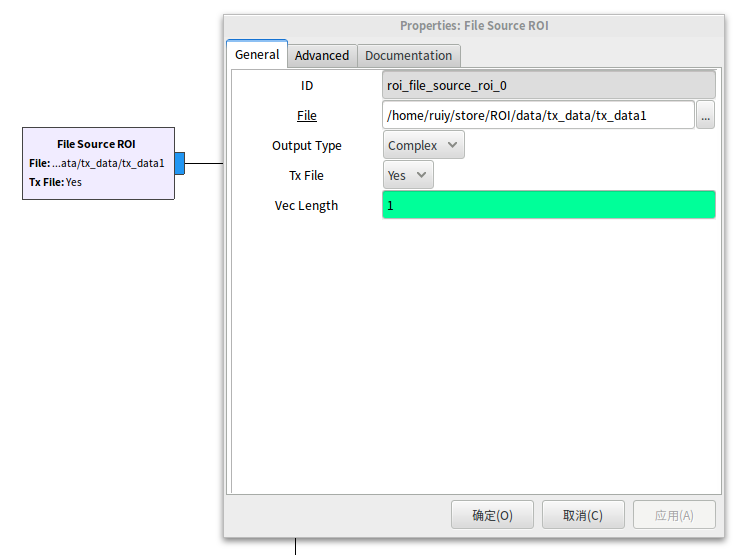
\includegraphics[width=0.9\textwidth]{images/file_source_roi}
    \caption{导频序列输出模块}{} 
    \label{file_source_roi}
\end{figure}

\subsection{数据发射模块}

% 参考 https://zhuanlan.zhihu.com/p/24217098

数据发射模块是直接使用了GNURadio自带的模块$UHD: USRP\quad Sink$,其属于GNURadio的$gr-uhd$系列,该模块用于将数据采样点送入USRP设备中,USRP设备会将其调制发射到指定频率。其参数如图\ref{usrp_sink}所示。

该模块实际是计算机端的控制平台,其实际执行是由USRP中的FPGA以及相关器件实现实现。该模块需要将基带数据通过USB口或者网口送入到USRP中去,如图\ref{usrp_sink_theory}所示为PC端与USRP端的交互。该模块属于计算机端的上层应用程序,使用C++或者Python编写,调用UHD驱动程序和系统调用,控制硬件接口的数据读写。PC与USRP的交互使用USB3.0或者以太网网口,目前大部分外设均使用USB3.0或者千兆以太网网口传输数据,来保证输出速率,满足实时性,USB3.0的速率可达到500MBps\cite{wei2016software}。

在发射数据时,进程从用户态切换到内核态,通过系统调用控制网卡或USB的读写。通过以太网网口或者USB口,将数据送入到USRP内部。USRP内部的处理分为三个部分。

\begin{itemize}
    \item 首先,发送控制模块和数字上变频模块(DUC)为了处理速度足够快,采用FPGA实现。发送控制模块控制USRP的发送时序。DUC模块用于基带数据上变频到中频\cite{xiong2015open}。
    \item 其次,中频数字信号经过DAC器件数模转换得到模拟域的数据,再进一步进行模拟域的信号处理
    \item 模拟域中,信号先经过低通滤波器得到更加平滑的信号,再与晶振信号相乘,将中频信号调制到指定射频频点,最后射频信号经过功率放大器发射出去。
\end{itemize}


\begin{figure}
    \centering
    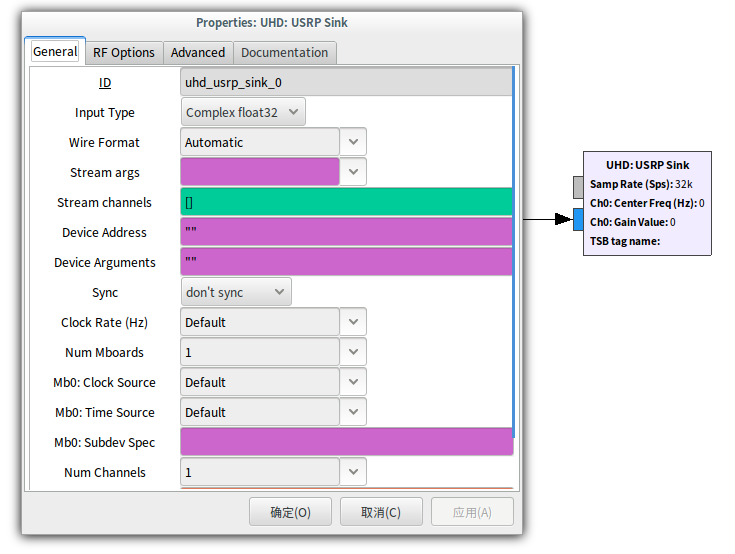
\includegraphics[width=0.9\textwidth]{images/usrp_sink}
    \caption{数据发射模块}{} 
    \label{usrp_sink}
\end{figure}

\begin{figure}
    \centering
    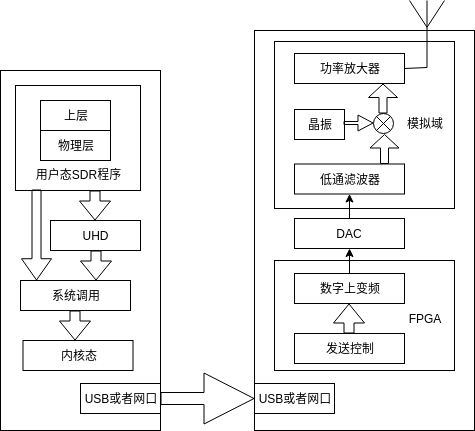
\includegraphics[width=0.9\textwidth]{images/usrp_sink_theory}
    \caption{数据发射时USRP内部示意图}{} 
    \label{usrp_sink_theory}
\end{figure}

\subsection{数据接收模块}

数据接收模块也是直接使用了GNURadio内置的模块,同属于$gr-uhd$的模块集,该模块和$UHD: USRP\quad Sink$作用相反,其作用是通过USB口或者千兆以太网网口从USRP中获取基带数据,并送入到输出端口。其参数如图\ref{usrp_source}所示。

\begin{figure}
    \centering
    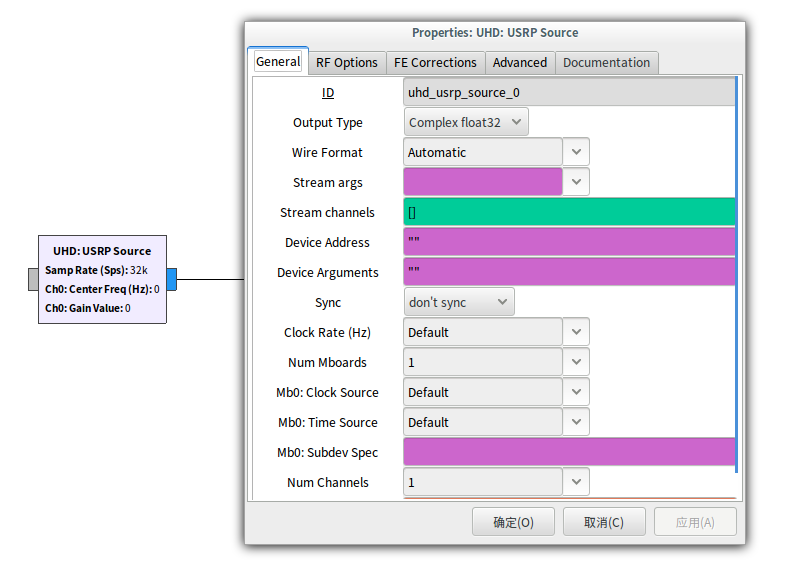
\includegraphics[width=0.9\textwidth]{images/usrp_source}
    \caption{数据接收模块}{} 
    \label{usrp_source}
\end{figure}

和$UHD: USRP\quad Sink$类似,该模块属于进程中的用户态部分,其在运行时会切换到内核态,并从与USRP相连接的以太网网口或者USB口读取高速数据。如图\ref{usrp_source_theory}所示为USRP在接收数据时与PC的交互。在接收数据时,USRP外设同样分为三个阶段处理信号,

\begin{itemize}
    \item 首先,信号经过低噪声放大器,避免将噪声放的过大。之后与晶振信号相乘,下变频到中频,再通过低通滤波器使得信号更加平滑。
    \item 其次,中频模拟信号通过ADC器件模数转换为数字信号。再进一步进行数字域的处理。
    \item 中频数字信号通过数字下变频,得到基带信号,再通过接收控制模块。为了速率保障,数字下变频模块和接收控制模块同样使用FPGA实现,接收控制模块控制USRP的接收行为。
\end{itemize}

USRP处理得到数字基带信号之后,通过以太网网口或者USB口,将数据送入PC中并触发中断,或者通知上层程序数据可读。PC中的上层程序陷入内核态,调用UHD驱动程序和系统调用从以太网网口或者USB口读取数据,然后返回用户态进一步处理数据。

\begin{figure}
    \centering
    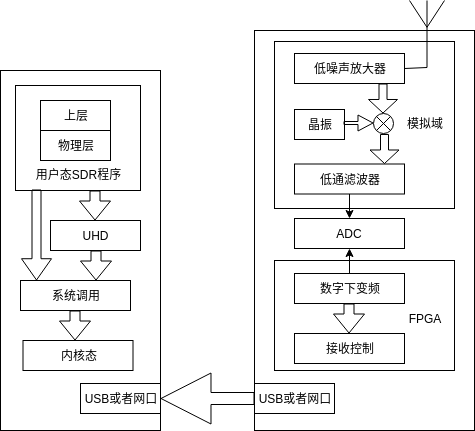
\includegraphics[width=0.9\textwidth]{images/usrp_source_theory}
    \caption{数据接收时USRP内部示意图}{} 
    \label{usrp_source_theory}
\end{figure}

\subsection{导频信号检测模块}

导频信号检测模块从数据接收模块中读取基带数据流,并按照上述粗同步的方式,通过fft检测指定间隔的两段信号是否为指定频率的正弦波,若是,则判断为需要检测的导频信号,将其转存到磁盘上,供之后信道估计使用。这种类型模块在GNURadio称作输入模块,输入模块无输出端口、有输入端口。

本文在设计该模块时提供了诸多模块参数,如图\ref{file_sink_roi}所示。其中各参数的意义为,

\begin{itemize}
    \item $Sine Freq$为该模块需要检测的导频信号首尾两端正弦波的频率
    \item $Threshold$为通过fft判断能量时所用阈值
    \item $FFT Size$为检波是所做fft长度
    \item $Rev-Send latency$为检测到导频信号与回发导频信号之间的时间间隔
\end{itemize}

通信双方的收发机中都有该模块。不同的是,当该模块检测到对端发射的导频信号,Bob会触发信号事件,将导频序列输出模块中的$Tx\_File$设置为$True$,发射Bob端的导频信号。Alice的导频信号检测模块收到Bob发射的导频信号之后,并不会再次发射信号,而是继续本次信道探测的后续过程,直到该次密钥生成过程完成,上层程序才会控制导频序列输出模块再次发射信号。

\begin{figure}
    \centering
    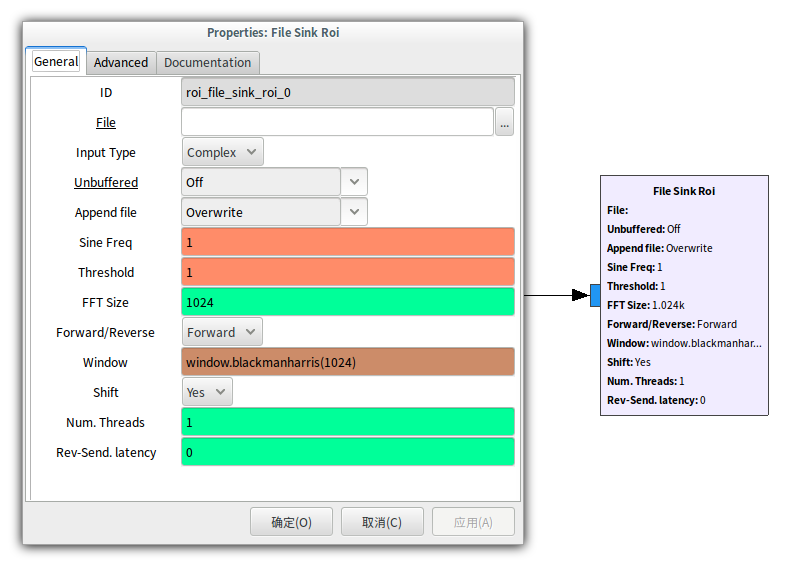
\includegraphics[width=0.9\textwidth]{images/file_sink_roi}
    \caption{导频信号检测模块}{} 
    \label{file_sink_roi}
\end{figure}

\subsection{导频信号收发机的整体结构}

本文基于上述四个GNURadio模块搭建导频信号收发机,整体结构如图\ref{two_tranceiver_structure2}所示。上层程序通过控制Alice的导频序列发射模块,发射导频信号,将导频信号调制到指定频点,并通过USRP射频前端发射导频信号。Bob使用导频信号检测模块不断检测导频信号,当检测到指定导频信号时,转存到磁盘,并触发导频信号发射事件,通知发射机中的导频序列发射模块发射导频信号,Bob端的发射机发射导频信号之后,Alice端接收机中的导频信号检测模块可以检测到Bob端发射的导频信号,并转存导频信号到磁盘。一次信道探测过程完成。

实际上,检测算法由于阈值设定过高或者过低,有可能检测不到对方发射的导频信号或者将错误的信号数据误认为导频信号。因此Alice端设计了重发机制。在一次信道探测过程中,Alice会每隔一定时间,重新发射一次导频信号,直到检测到Bob回发的导频信号。

\begin{figure}
    \centering
    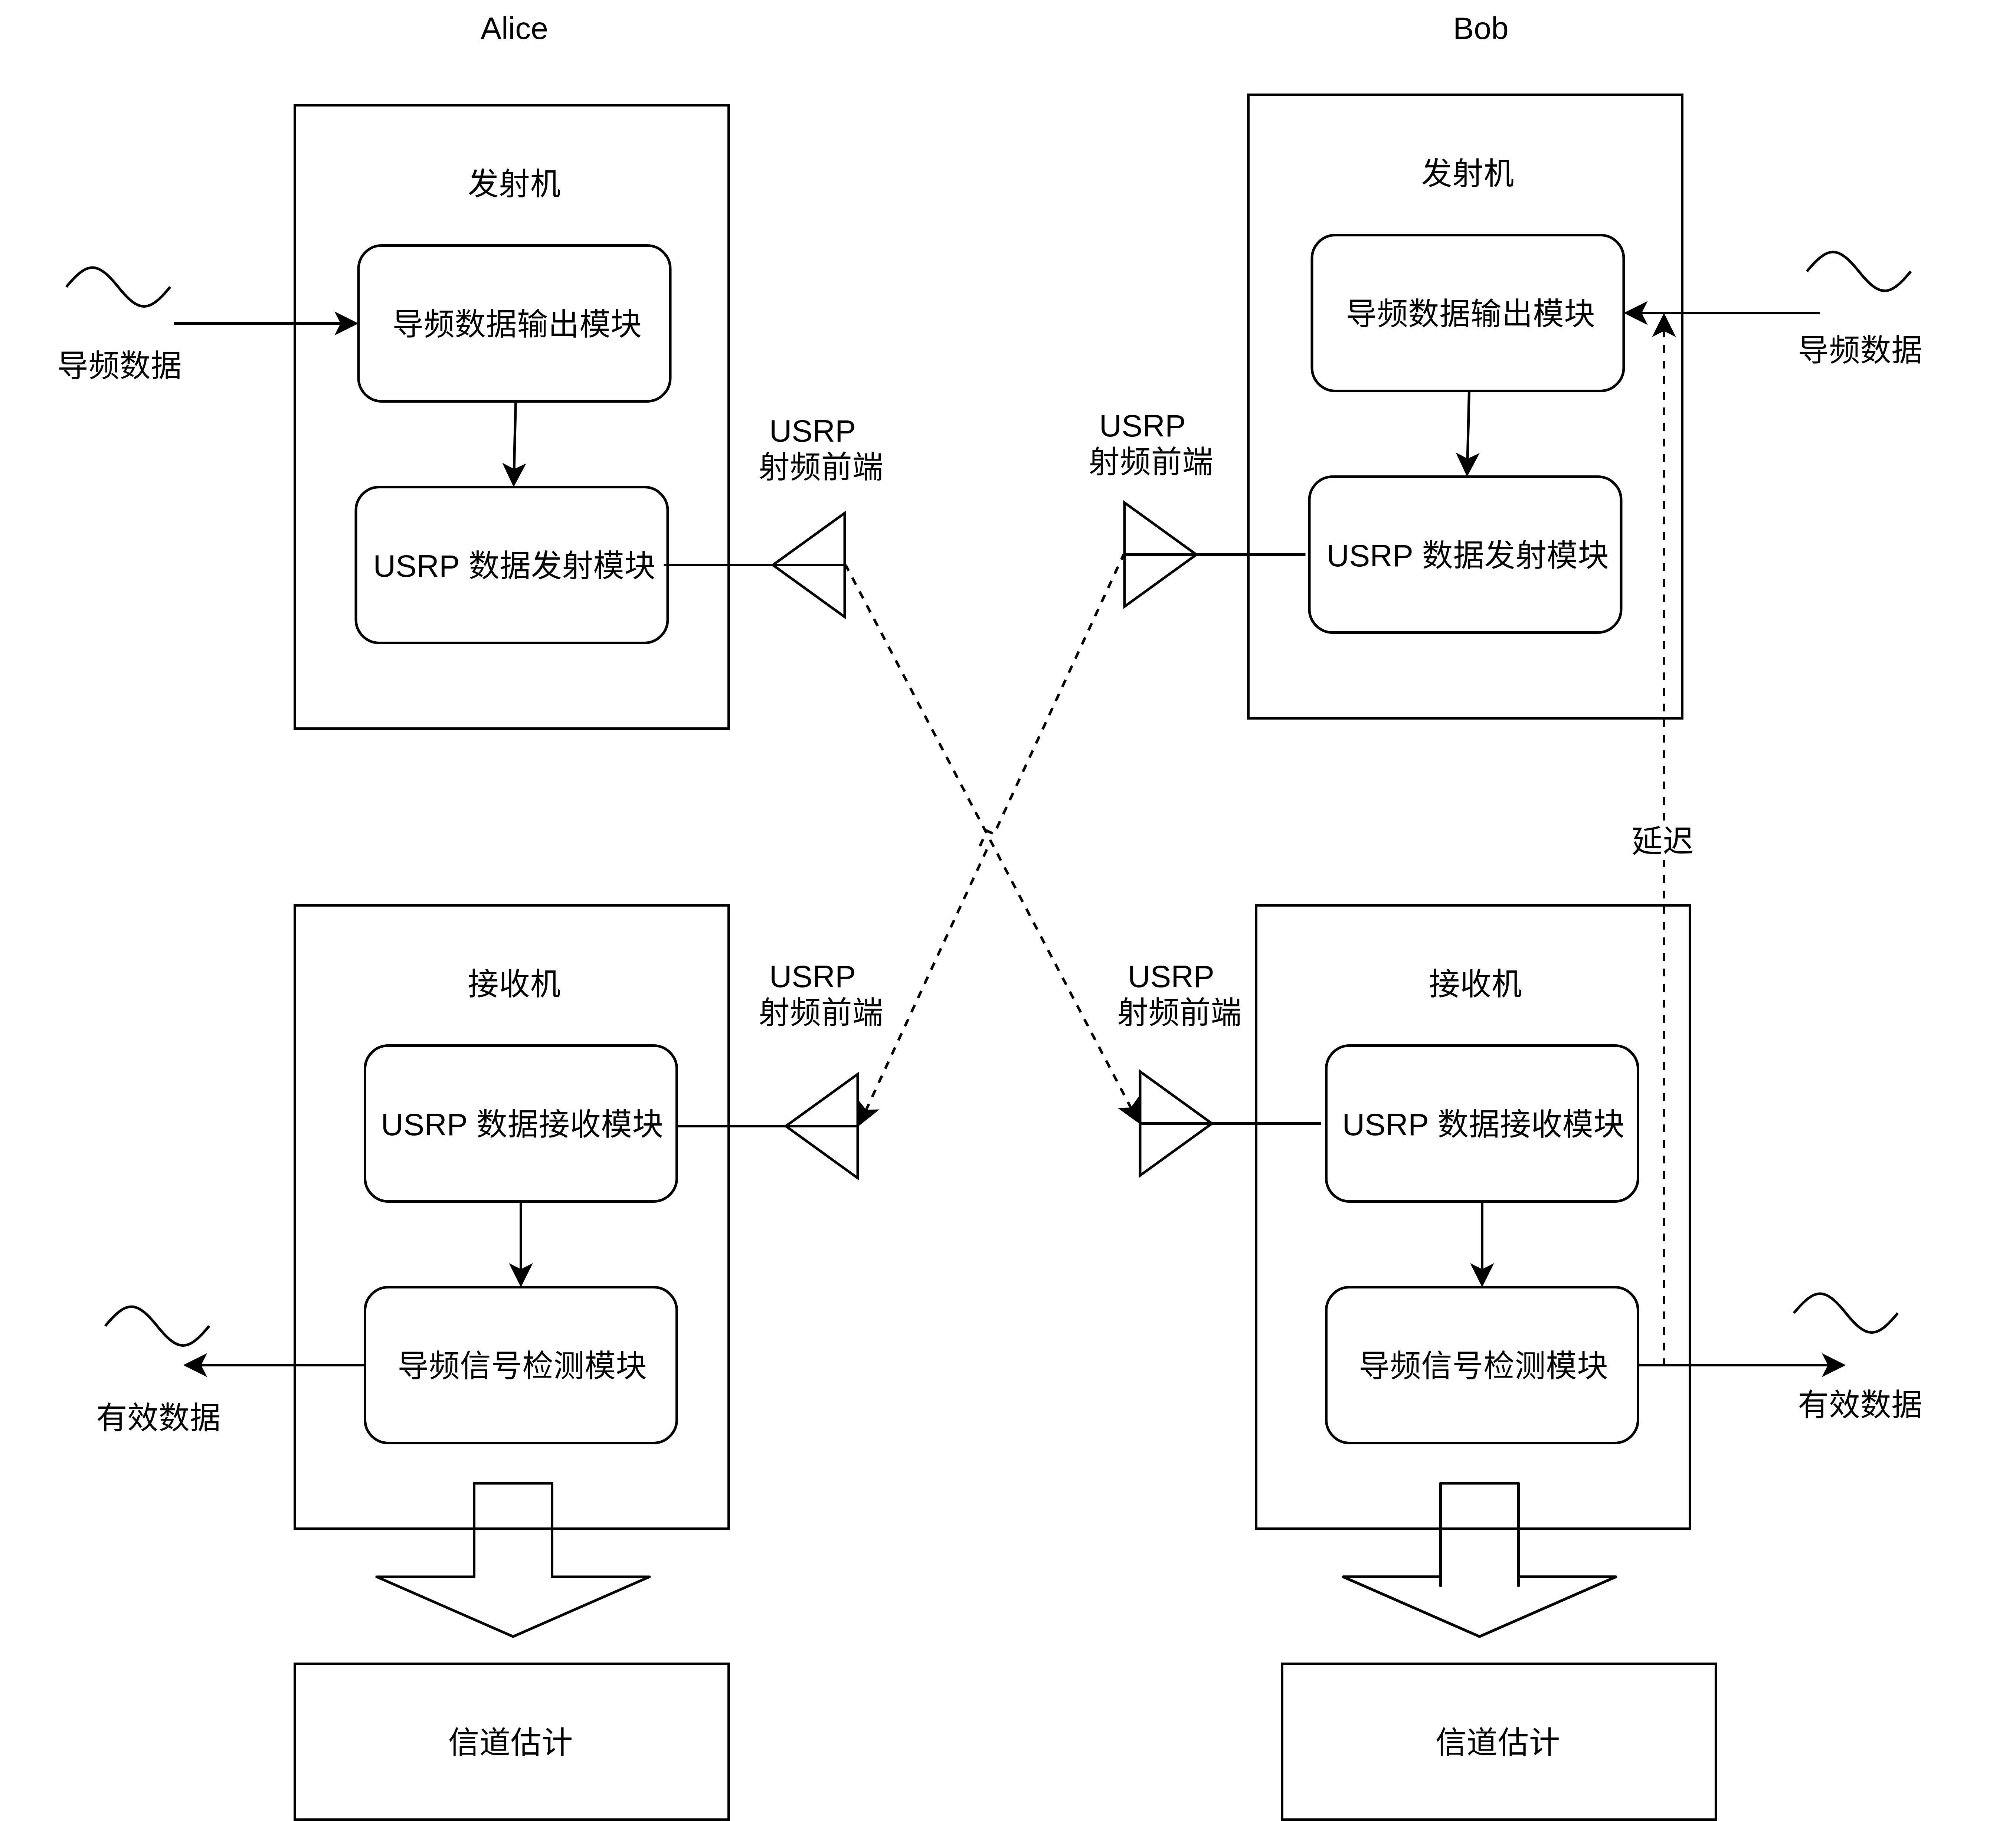
\includegraphics[width=0.9\textwidth]{images/two_tranceiver_structure2}
    \caption{TDD导频收发机设计}{} 
    \label{two_tranceiver_structure2}
\end{figure}

\chapter{无线信道密钥生成流程}

本章将详细的介绍无线密钥生成系统设计和实现的具体细节,介绍上层应用利用导频信号收发机实现信道探测的过程。% TODO 补完介绍

\section{TDD/FDD系统信道探测系统研究设计}

在上一章节中,本文介绍了如何利用GNURadio设计密钥生成系统所需要的模块搭建导频信号收发机,导频信号收发机使用如图\ref{tranceiver_structure}四个模块完成TDD/FDD系统中信号的发送和接收。

\begin{figure}
    \centering
    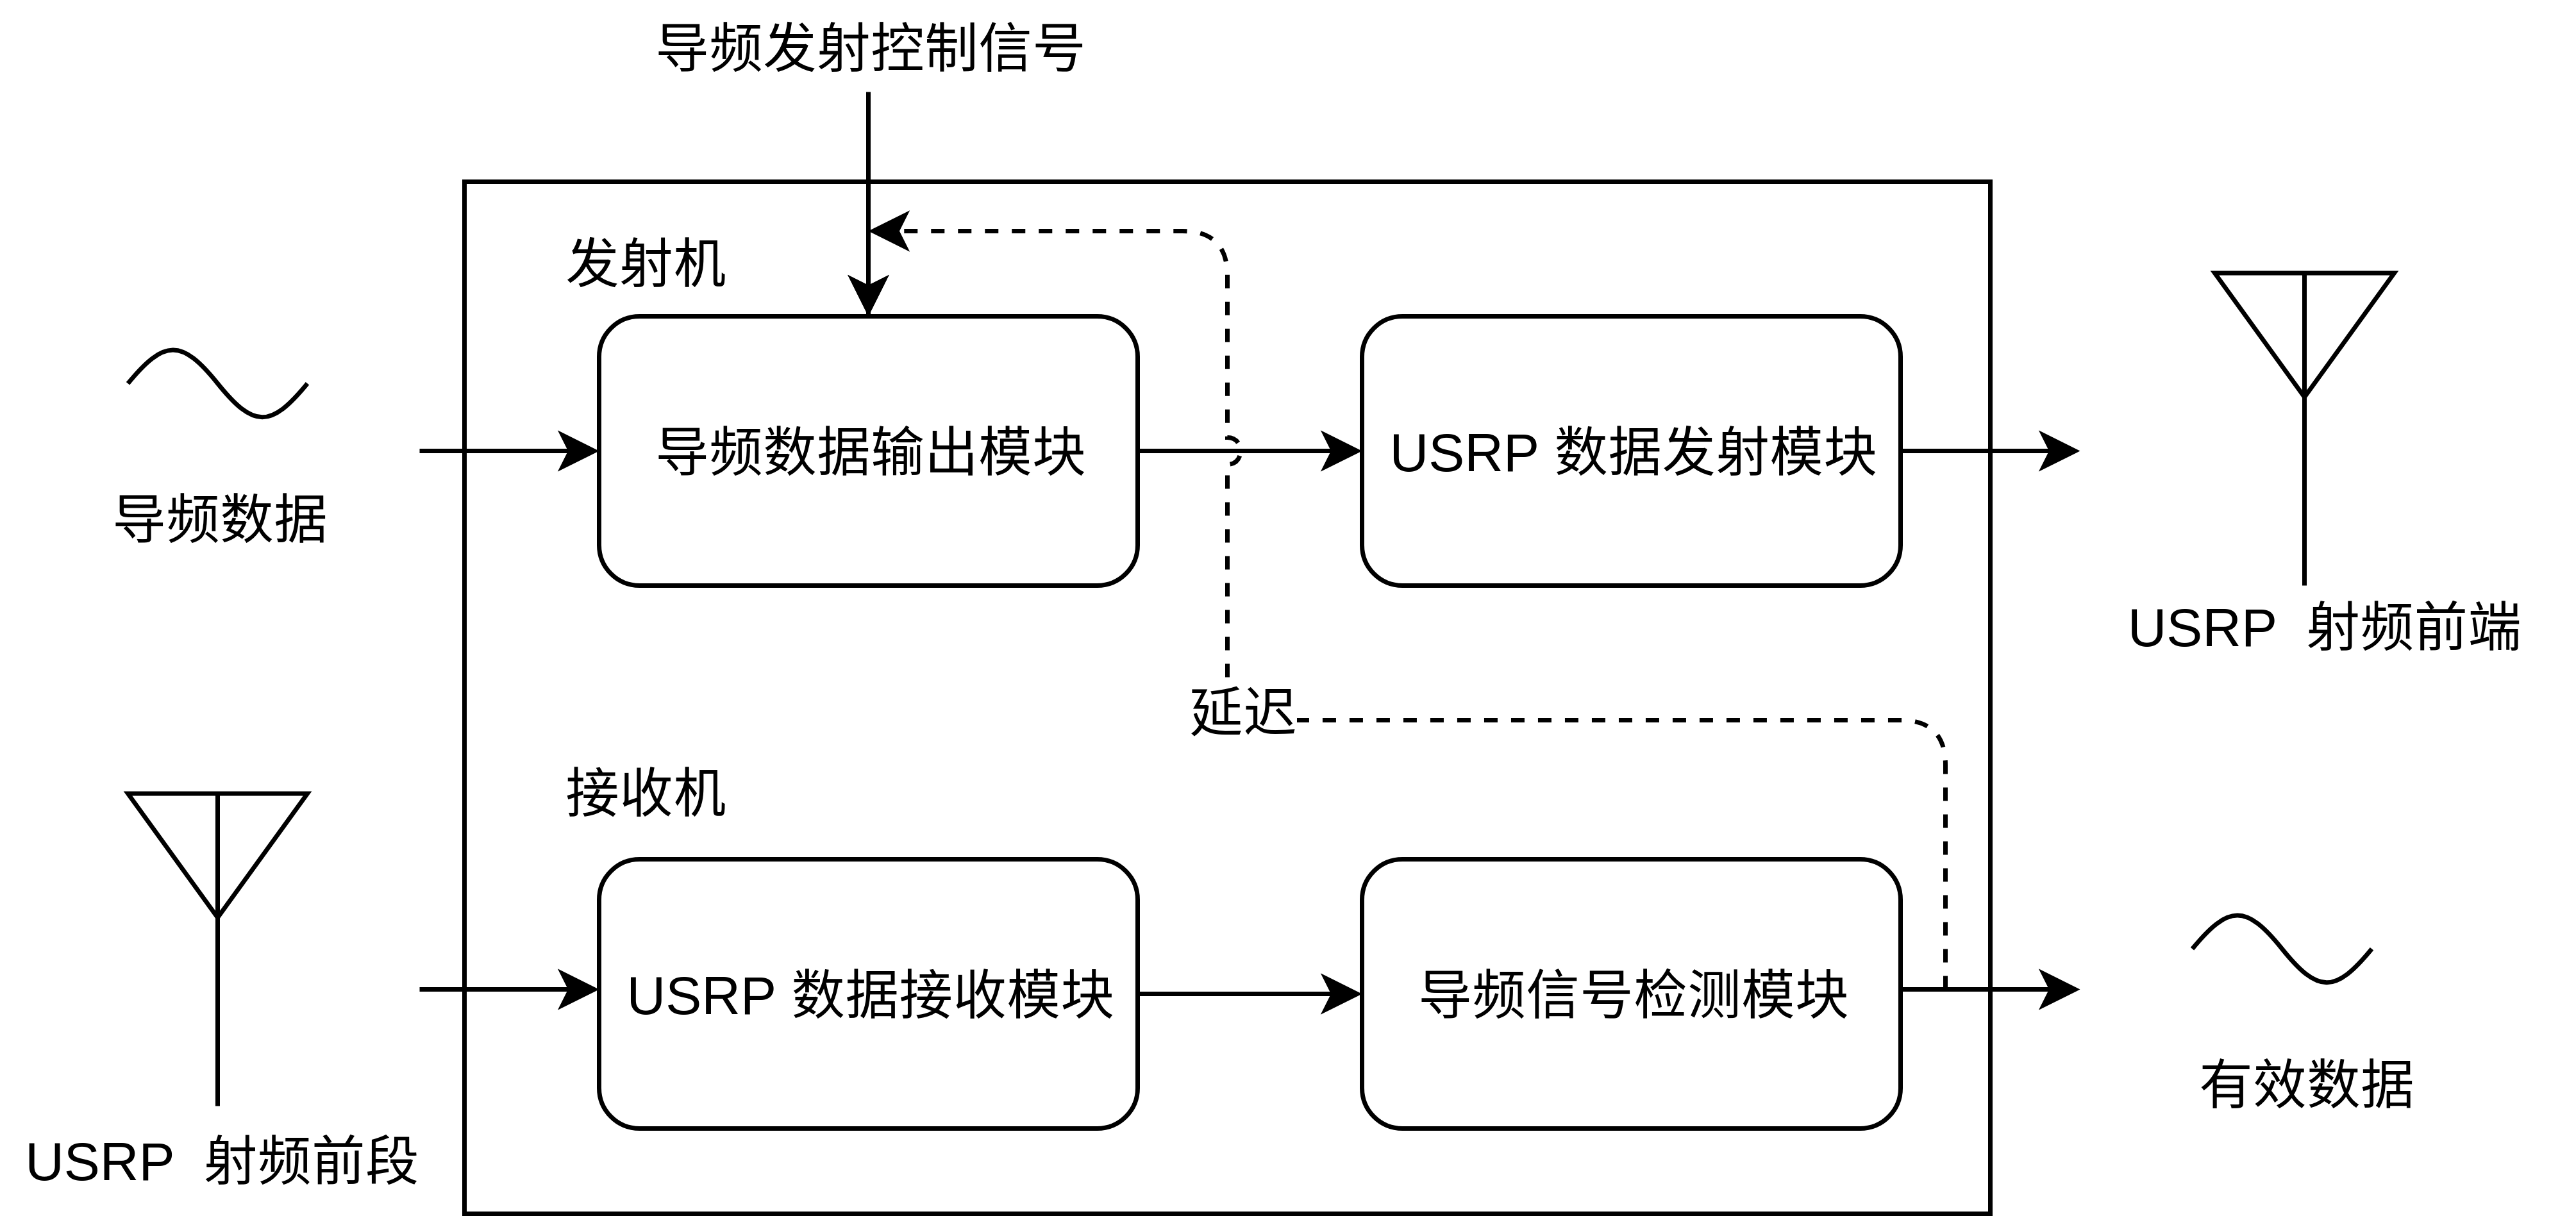
\includegraphics[width=0.9\textwidth]{images/tranceiver_structure}
    \caption{导频信号收发机}{} 
    \label{tranceiver_structure}
\end{figure}

对于TDD系统来说,Alice与Bob之间的信道探测过程如图\ref{two_tranceiver_structure}所示。对于FDD系统来说,Alice与Bob之间的信道探测过程如图\ref{two_tranceiver_structure2}所示。TDD和FDD系统中不同的地方在于,TDD系统的通信双方在同一个频点上发射和接收导频信号,而FDD系统的通信双方在不同的频点上发射和接收导频信号。


\begin{figure}
    \centering
    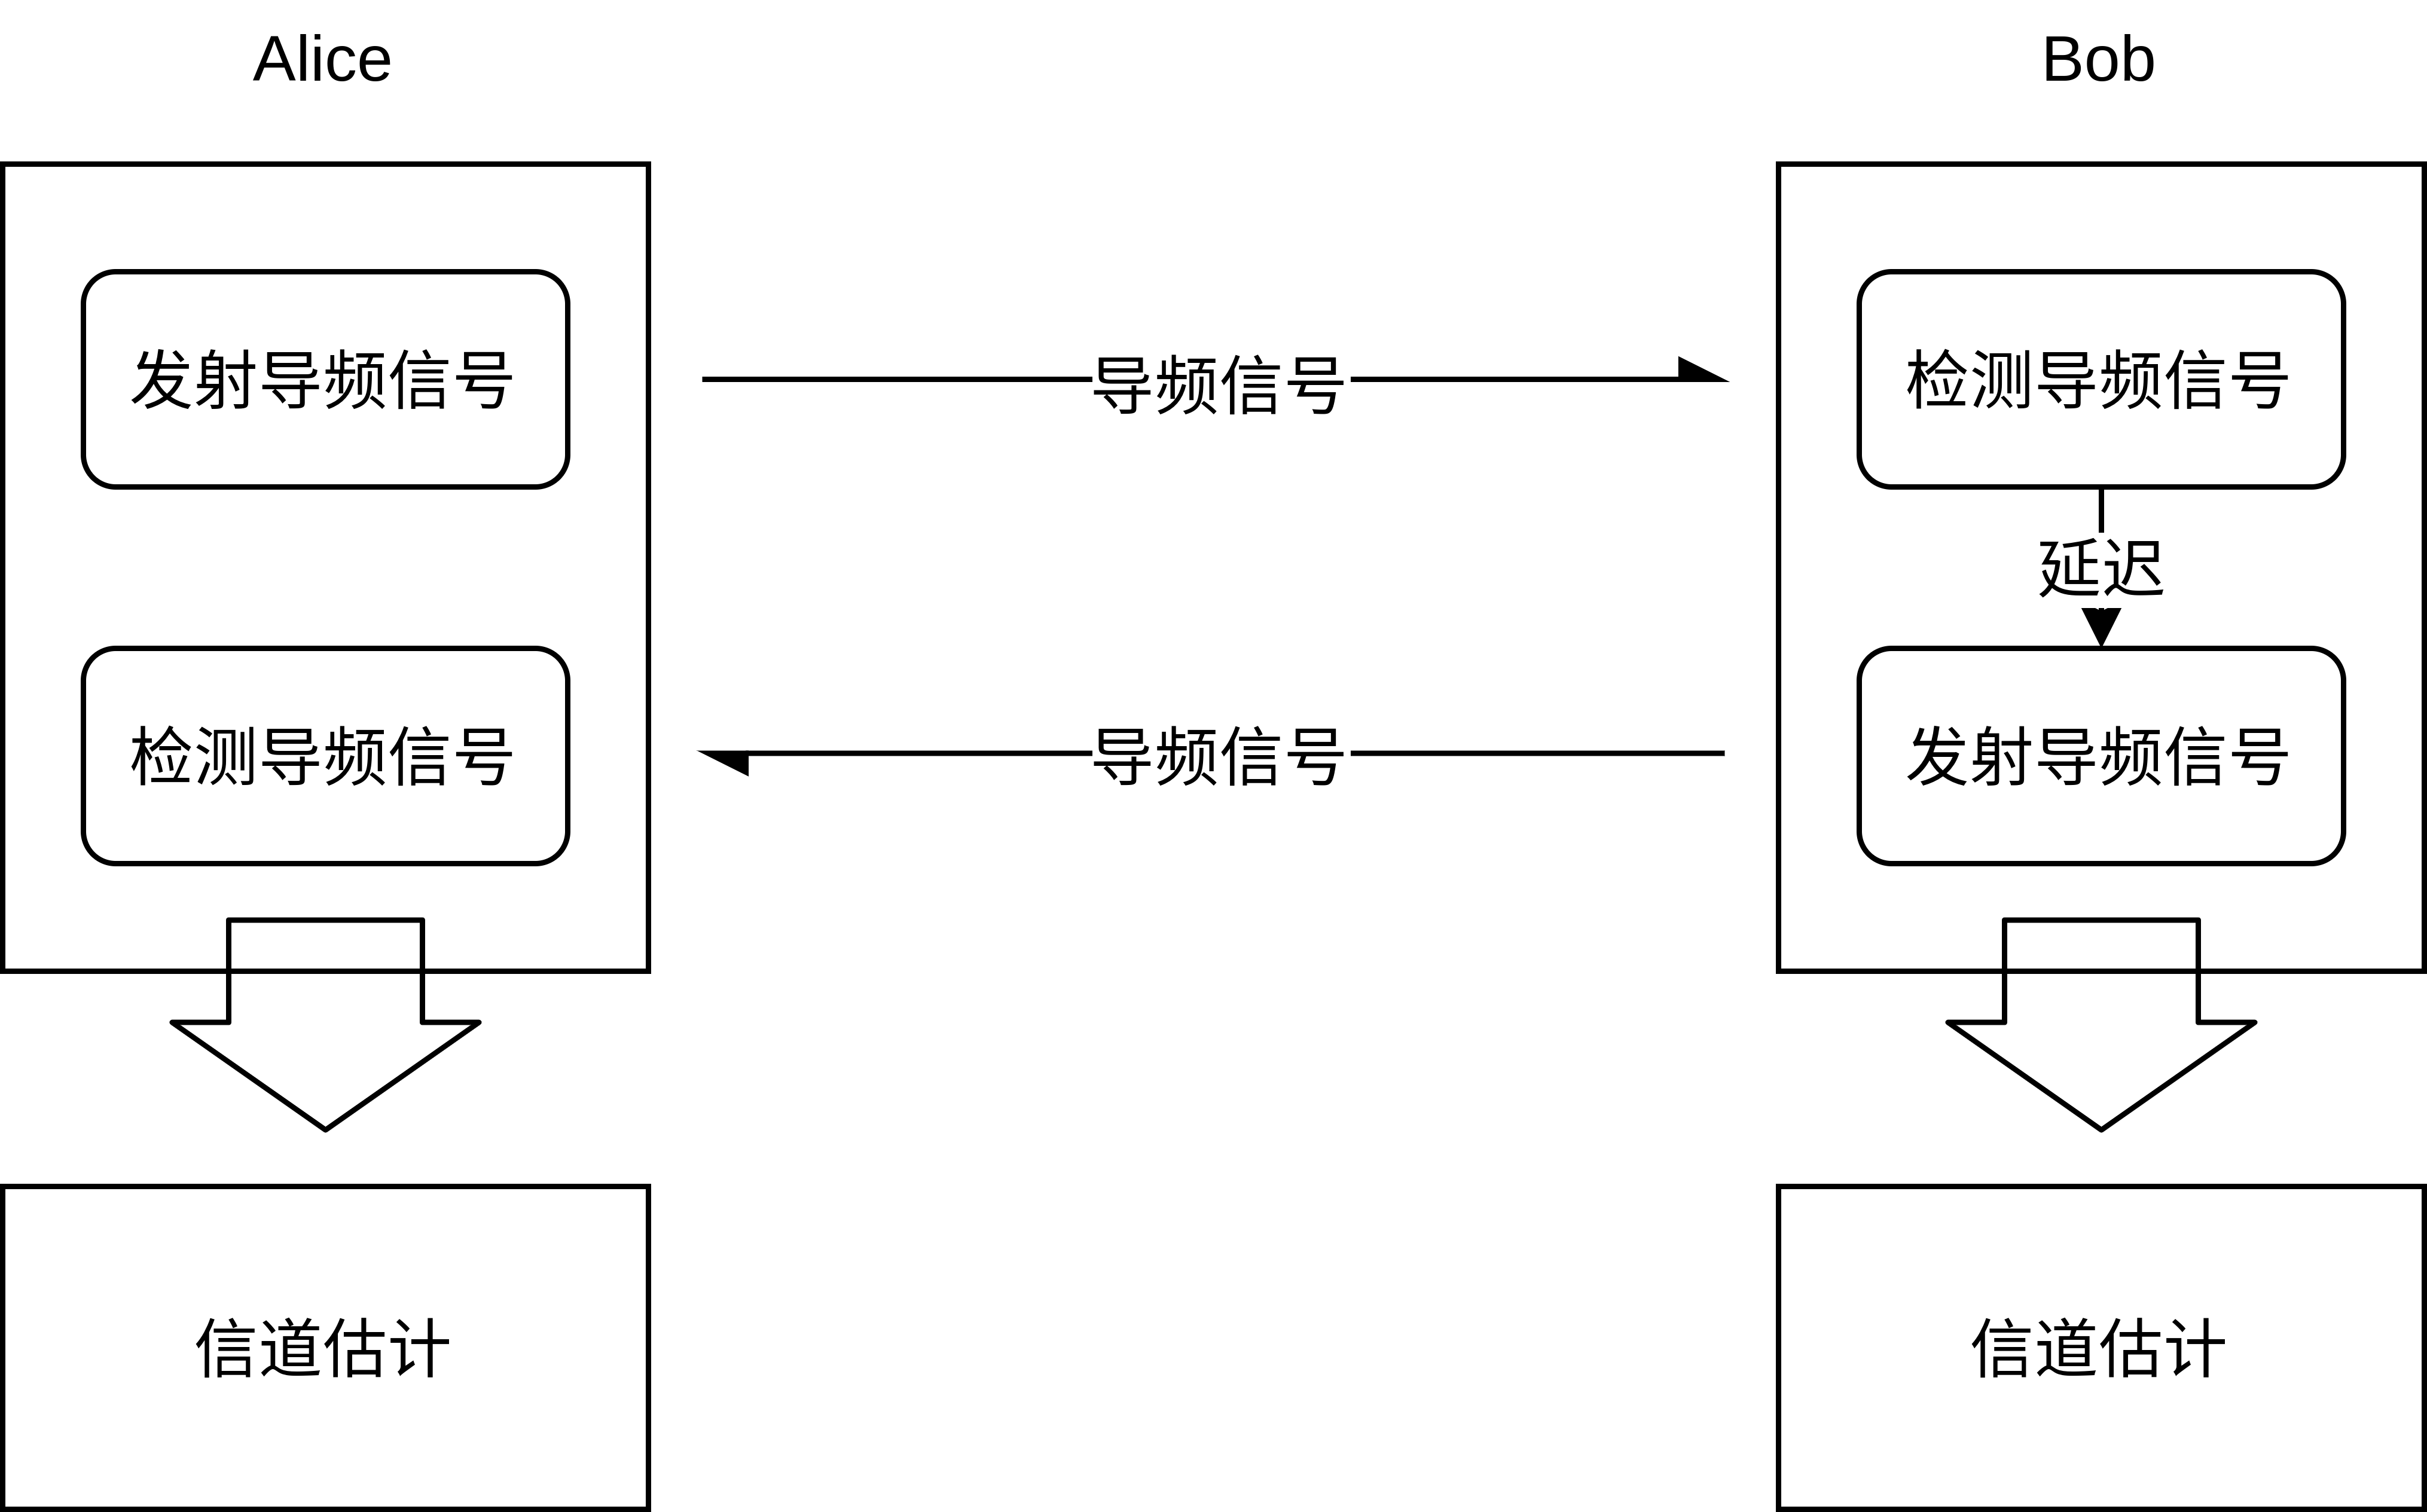
\includegraphics[width=0.9\textwidth]{images/two_tranceiver_structure}
    \caption{TDD系统中的信道探测}{} 
    \label{two_tranceiver_structure}
\end{figure}

\begin{figure}
    \centering
    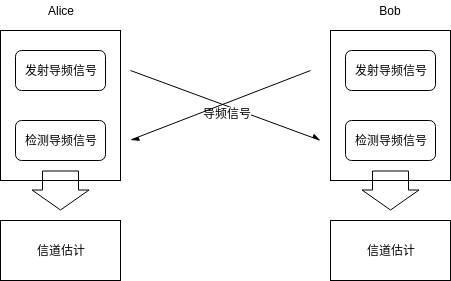
\includegraphics[width=0.9\textwidth]{images/two_tranceiver_structure_fdd}
    \caption{FDD系统中的信道探测}{} 
    \label{two_tranceiver_structure_fdd}
\end{figure}

TDD系统中,通信双方分Master和Slave端。Slave端的检波模块只有检测到Master端发射的导频信号,才会发射导频信号,因此Slave端的导频信号检测模块和导频序列输出模块之间存在信号事件。FDD系统中,通信双方的地位是对等的,不分主从,Slave发射导频信号是不受Master影响的,因此导频信号检测模块和导频序列输出模块之间也不存在信号事件。

为了实现信号事件,本文使用GNURadio中$gr::basic_block$提供的消息传递接口。在GNURadio中,$gr::basic_block$是所有模块的父类,模块也会区分输入和输出端口。该类提供了消息订阅与通知机制,如果某个模块注册了某个端口,那么当该模块在该端口发布消息时,任何订阅该模块同名端口的模块都会收到该消息并根据消息类型作出不同的响应行为。实际上,当模块在某端口发布消息时,该模块会迭代所有订阅同名端口的模块,并调用成员方法将消息压入到订阅模块的消息队列中去,如图\ref{message_passing}所示。本文实现了导频信号检测模块和导频序列输出模块之间的消息通知,并加入延迟这一参数观察不同延迟时间下信道和密钥生成的结果。

\begin{figure}
    \centering
    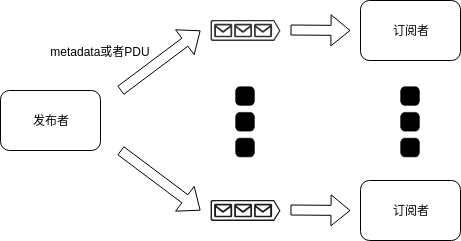
\includegraphics[width=0.9\textwidth]{images/message_passing}
    \caption{消息传递接口}{} 
    \label{message_passing}
\end{figure}

\section{信道估计}

本文使用的导频信号如图\ref{tx_pilot}所示,系统检波得到的导频信号如图\ref{rx_pilot}所示。在密钥生成协议中,通信双方均已得知导频信号的组成部分,因此可以通过已知导频信号和接收导频信号估计得到信道。

\begin{figure}
    \centering
    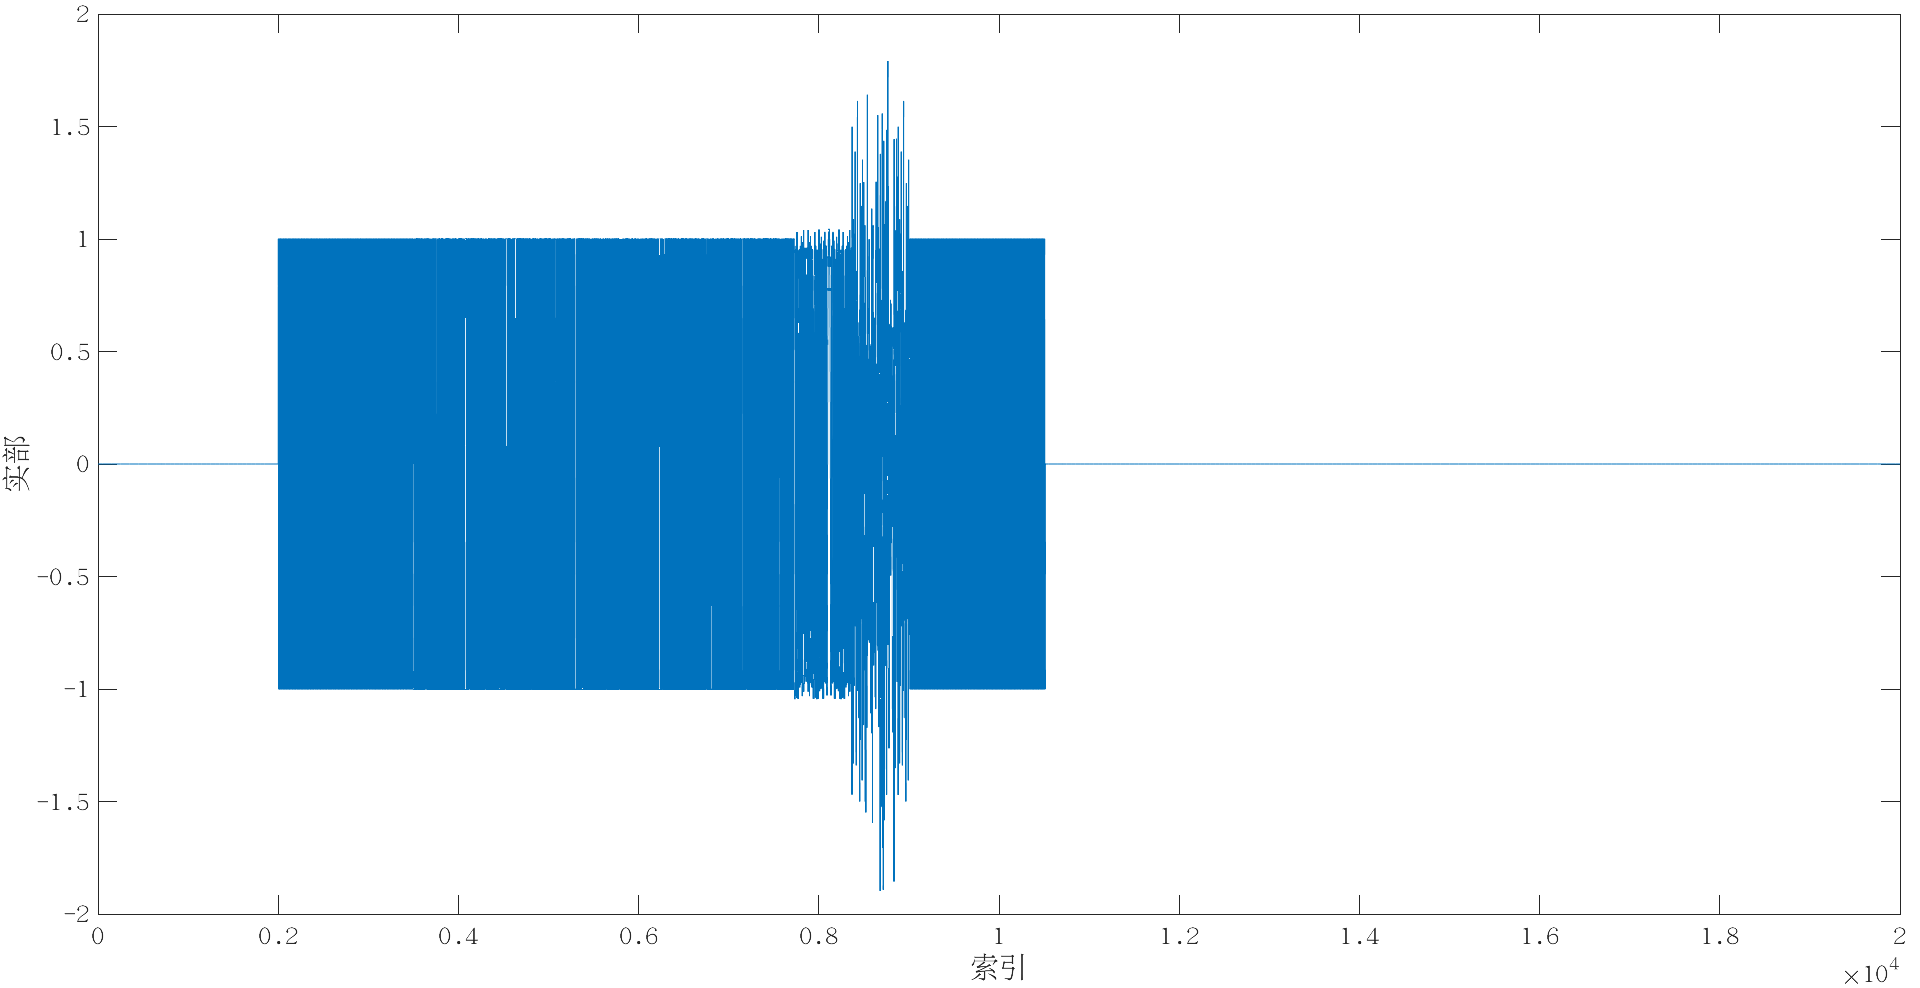
\includegraphics[width=0.9\textwidth]{images/tx_pilot}
    \caption{发射导频信号}{} 
    \label{tx_pilot}
\end{figure}

\begin{figure}
    \centering
    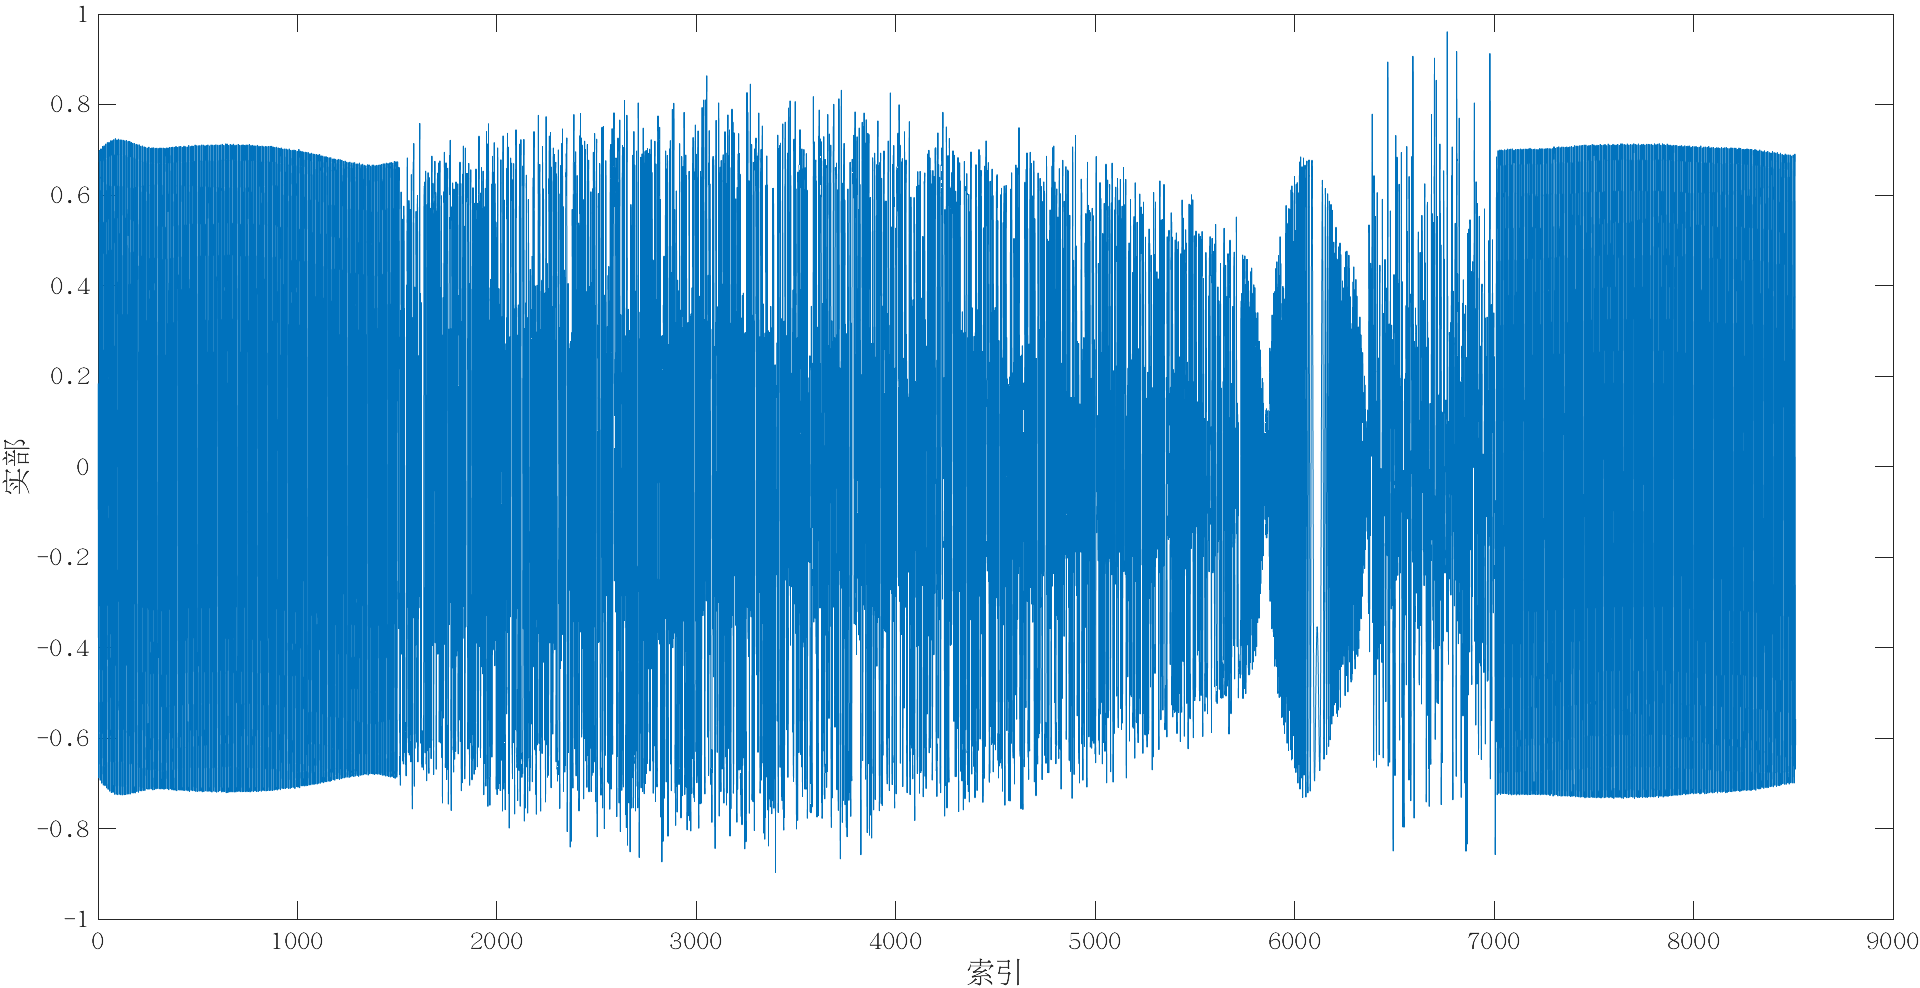
\includegraphics[width=0.9\textwidth]{images/rx_pilot}
    \caption{接收导频信号}{} 
    \label{rx_pilot}
\end{figure}

假设某通信方发射的导频信号$P(k)$,则其数据成分依次为表\ref{component_of_pilot}所示。空数据点是为了避免USRP发射导频信号时初始数据点增益较小的可能,首尾两端正弦波用于粗同步,m序列cp前缀是避免干扰,m序列用于精同步和信道估计。

\begin{table}[]
    \centering
    \begin{tabular}{|l|l|}
    \hline
    组成成分 & 长度(复数点个数)\\ \hline
    空数据点 & 2000 \\ \hline
    首端正弦波 & 1504 \\ \hline
    m序列cp前缀 & 129 \\ \hline
    m序列 & $ 4095 = 2^{12} - 1 $ \\ \hline
    OFDM数据 & 1280 \\ \hline
    尾端正弦波 & 1504 \\ \hline
    \end{tabular}
    \caption{导频信号的组成成分
    \label{component_of_pilot}}
\end{table}

\subsection{频偏估计}

由于信道的非线性、收发两端晶振差异、移动环境中的多普勒频移,接收的导频信号需要进一步消除频率偏移。
在接收的导频信号中,可以使用首尾两端的正弦波来进行频偏估计。假设利用正弦波中的$Sine(k)$部分进行频率估计,对于间隔点数$\tau$来说,对载波频偏进行粗估计,有

\begin{align}
    z(\tau) & = \frac{1}{N - \tau} \sum_{i = 1}^{N-\tau} \bar{Sine(i)} \times Sine(i + \tau) \\
    & = \frac{1}{N-\tau} \sum_{i = 1}^{N-\tau} e^{-jwi\epsilon} e^{jw(i+\tau)\epsilon} \\
    & = \frac{1}{N-\tau} \sum_{i = 1}^{N-\tau} e^{jw\tau\epsilon}
\end{align}

本文计算了$L_{\tau} = 5$次粗估计,即$\tau \in \{1,..., L_{\tau}\}$,并求出相位值phase

\begin{equation}
    p(\tau) = \frac{1}{2\pi} tan^{-1} {\frac{Im(z(\tau))}{Re(z(\tau))}}
\end{equation}

并将$p(\tau)$序列通过$\pm \pi$调整成递增或者递减序列$\tilde{p(\tau)}$,并除以对应的间隔点长度$\tau$,得到补偿因子序列为,

\begin{equation}
    \epsilon(\tau) = \tilde{p(\tau)} / \tau
\end{equation}

最终频率补偿因子为$\epsilon(\tau)$的平均值$\bar{\epsilon}$,并通过其方差判断该补偿因子是否误差较大,如果较大则舍弃不用。因为有首尾两段正弦波,通过这两端正弦波分别估计出$\bar{\epsilon}_1$和$\bar{\epsilon}_2$,以及对应的方差$\sigma_1$和$\sigma_2$。如果$\sigma_1$和$\sigma_2$均大于阈值$Threshold_{\sigma}$,则取其平均数作为补偿因子;如果$\sigma_1$和$\sigma_2$均小于阈值$Threshold_\sigma$,则均舍弃不用;如果一大一小,则取其中满足大于阈值的因子作为补偿因子。

另外可以利用两端正弦波一起做频偏估计,即对相隔距离为$\tau_{12}$、长度均为$N$的正弦波$Sine_1$和$Sine_2$综合起来作,

\begin{equation}
    z = \frac{1}{N} \sum_{i=1}^N Sine_1(i) \times \tilde{Sine_2(i)}
\end{equation}

由于,

\begin{equation}
    Sine_2(i) = Sine_1(i - \tau{12})
\end{equation}

则

\begin{align}
    z = & \frac{1}{N} \sum_{i=1}^N e^{-jwi\epsilon} e^{jw(i+\tau_{12})\epsilon} \\
      = & \frac{1}{N} \sum_{i=1}^N e^{jw\tau_{12}\epsilon} \\
\end{align}

\begin{equation}
    p = \frac{1}{2\pi} tan^{-1} \frac{Im(z)}{Re(z)} 
\end{equation}

\begin{equation}
    \epsilon = p / \tau_{12}
\end{equation}


\subsection{信道补偿}

通过频偏估计得到补偿因子$\epsilon$,本文采用频率补偿的方法是直接对原信号补偿,即在离散傅里叶变换进行频率偏移的补偿,则对信号$S(k)$补偿的结果为,

\begin{equation}
    \tilde{S(k)} = S(k) * e^{2\pi \epsilon k}
\end{equation}

\subsection{信道估计}

从频偏补偿之后的导频信号中截取m序列$\tilde{m(k)}$,并和已知原始信号$m(k)$进行信道估计,

\begin{equation}
    h(k) = \sum_{i=1}^{L_m} \tilde{m(i)} \times m( (i + k) mod L_m )
\end{equation}

通过fft得到频域响应,然后移除直流分量,再滑动平均,最终得到信道估计的结果。

\begin{equation}
    H(k) = MA(FFT(h(k)))
\end{equation}

如图\ref{ma_before_after_res}是平滑前和平滑后的频率响应结果。

% /home/ruiy/store/data/experiment/indoor-no-move-600/alice/2019-04-01-10-48-12/csi 
\begin{figure}[htbp!]
    \centering 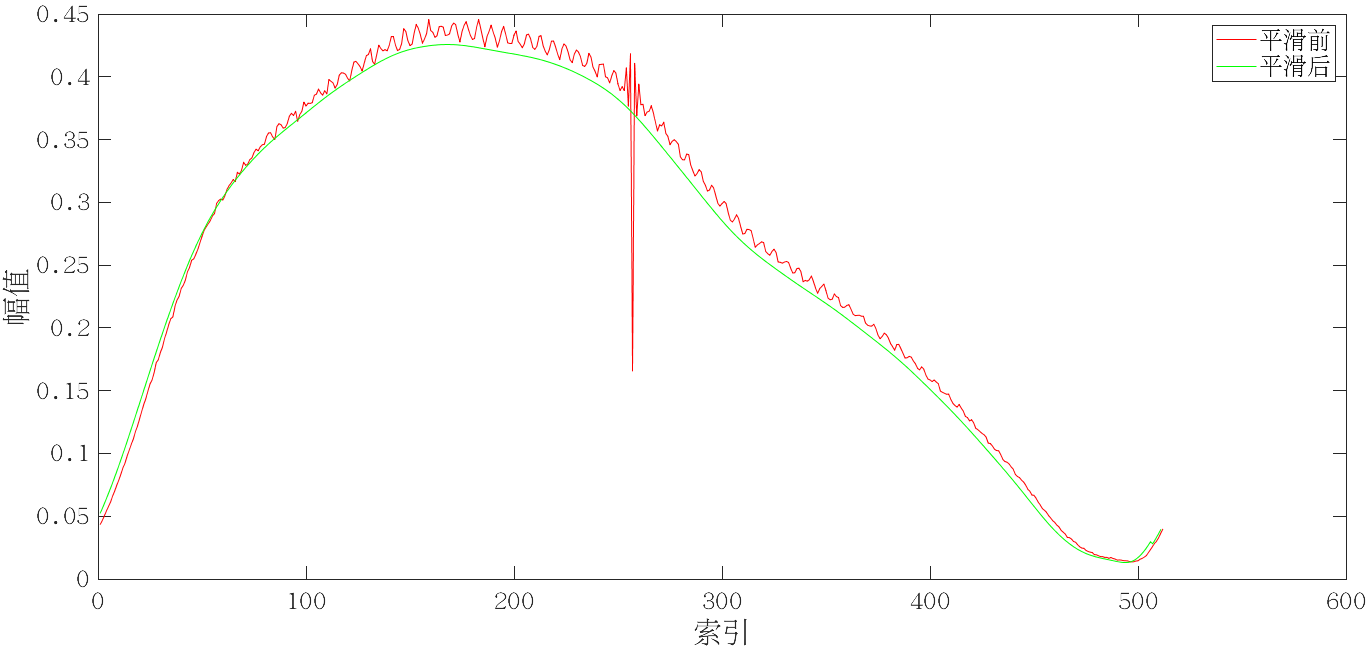
\includegraphics[width=0.9\textwidth]{images/ma_before_after_res} 
    \caption{平滑前后CSI结果}
    \label{ma_before_after_res}
\end{figure}

\section{特征量化}

对CSI进行降采样一方面可以提高密钥一致率,另一方面可以降低密钥泄露率。降采样之后,再进行归一化处理。本文先将CSI归一化到$[0, 2^L)$的范围内,并四舍五入得到整数值,其中L为整数。再除以$2^(L - R)$并向下取整得到最终量化值,其中R为量化阶数。

设CSI序列为$CSI(k)$,则首先归一化,

\begin{equation}
    Norm(k) = Round(\frac{(2^L - 1) CSI(k)}{Max(CSI)}
\end{equation}

再量化,

\begin{equation}
    Quant(k) = \frac{Norm(k)}{2^{(L - R)}}
\end{equation}

其中, $Round(\cdot)$为四舍五入,$Max(\cdot)$为取最大值

再进行格雷编码,减少比特的不一致率,最后再进行8b10b编码使得01比特的分布更加均匀、随机。

本文使用上述方式进行均匀量化,其中$L = 7$,$R = 3$,\ref{quantization_and_csi}所示为某次室外测量过程中,探测得到的CSI和其量化之后的部分结果。图中展示了通信双方Alice和Bob的CSI结果以及量化得到的部分比特流,可以看出Alice和Bob的CSI较为接近且生成的比特流相似,但是窃听者Eve测量得到CSI与合法通信方相差很大并且量化得到的比特流也相差较大。

\begin{figure}[htbp!]
    \centering 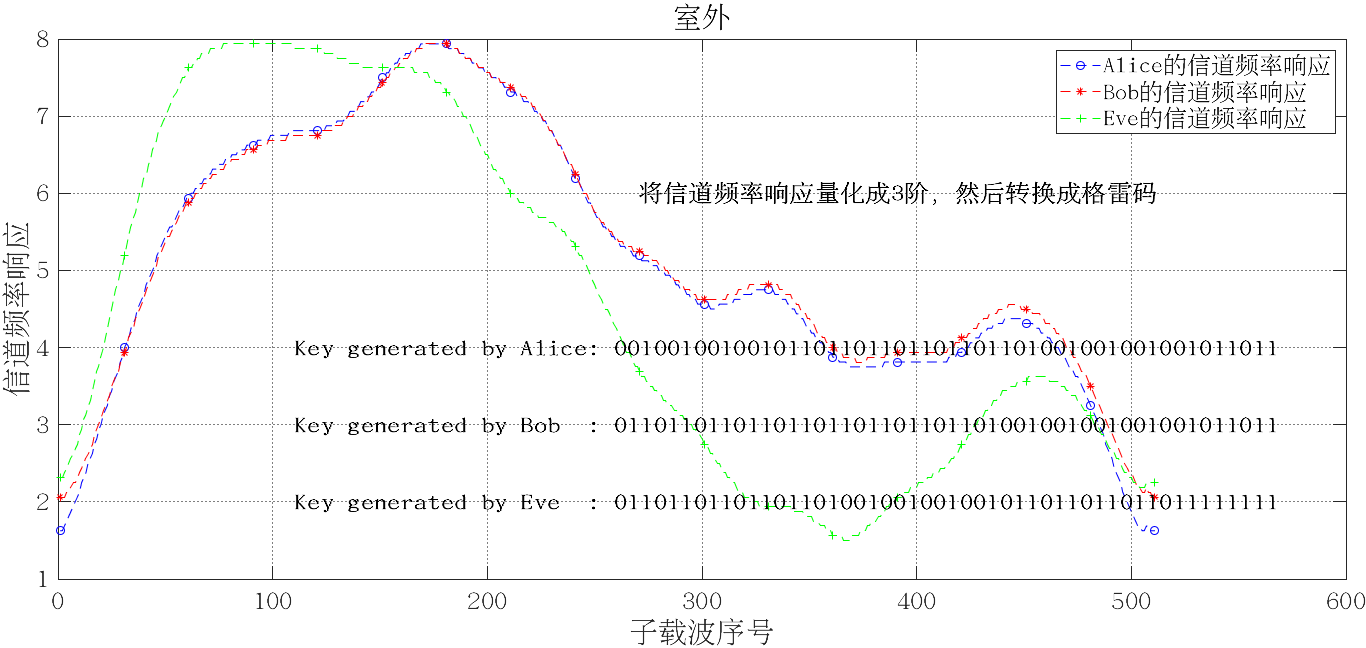
\includegraphics[width=0.9\textwidth]{images/quantization_and_csi} 
    \caption{量化之后的CSI}
    \label{quantization_and_csi}
\end{figure}

\section{信息调和}

在特征量化之后,通信双方需要进一步调和来消除密钥流中不一致的比特。在通信过程中,由于通信系统的上下行特性、硬件指纹、环境噪声等原因,通信双方测量得到的CSI虽然相似,却并不完全一致,进而导致生成密钥比特流中存在不一致的比特。因此需要通信双方结合信息调和来得到完全一直的比特流。本文实现了两种信息调和的方法。

一种是基于CRC校验的信息调和方法,这种方法通过对比特流分组,并对每组生成CRC校验码,通信双方比较每一组的校验码,校验码不一致的组直接舍弃、校验码相同的组保留。该方法的安全性取决于分组的大小,因为调和过程在公共信道进行,所以窃听者可以窃听到调和的信息并根据泄露信息预测出部分密钥的信息。对于本方法来说,由于公共信道上传递的是CRC校验冗余码,因此每组比特数越小,泄露的信息量就越小。

另外一种基于纠错码的信息调和方法,该方法将需要传递的会话密钥进行纠错编码,之后与特征量化步骤中生成的比特流一次异或加密,再通过公共信道发送给对方。对方收到之后同样先和比特流进行一次异或解密,再进行纠错解码,得到会话密钥。在特征量化步骤中,通信双方量化生成的比特流并不一致,该方法实际上将不一致的比特位当做信道过程中的干扰项,并基于纠错码的特点对不一致的比特进行纠错。当错误比特数超过纠错码性能时,接收方就无法正确恢复纠错码。为了接收方可以判断恢复得到的会话密钥的正确性,发送方在调和时会附带会话密钥的摘要,接收方在恢复出会话密钥之后,可以生成新摘要与其对比,便可以判断出是否纠正成功,如果纠错失败,则需要重新开始密钥协商过程。该方法同样存在调和过程中信息泄露的问题,分组过小,那么窃听者可以窃取更多的信息;分组过大,则纠错将会更加困难\cite{李古月2014无线信道的密钥生成方法}。

\subsection{基于CRC校验码的调和方法}

循环冗余校验(cyclic redundancy check, CRC)是一种错误检测方式,用于检测传输数据或者存储数据的意外更改。该方法将数据分块,并根据生成多项式作多项式除法得到校验冗余码。在检查时,会重复计算冗余码是否相同,如果冗余码不匹配,则说明数据被意外更改并进行纠错。

假设某长度为$L$数据块的多项式表示为$M(x)$,$M(x)$中多项式系数表示数据块中的每一位。$G(x)$为$n+1阶$的生成多项式,作为除数,用于生成校验冗余码。将$M(x)$各项同时乘以$x^n$,相当于在二进制字符串后面添加n个0,则$M(x) \cdot x^n$可以表示成,

\begin{equation}
    M(x) \cdot x^n = Q(x) \cdot G(x) - R(x) 
\end{equation}

其中$Q(x)$是除法结果,$G(x)$为除数,$R(x)$即所需校验冗余码。发送方会对每个数据块作相同处理,并将冗余码发送给接收方。接收方同样对数据分组,设相同位置的数据块为$M'(x)$,则检查$M'(x) * x^n + R(x)$是否可以被$G(x)$整除。如果可以整除,那么说明$M'(x)$与$M(x)$一致,那么该组数据块可以保留,否则舍弃不用。接收方以此方式对每组数据块作判断,最后得到校验结果向量$Vec(k)$,并传输给发送方,发送方再以此去除分组中校验不一致的组。

本文使用CRC-12校验,其生成多项式为$x^{12}+x^{11}+x^{3}+x^{2}+x+1$,对应字符串为$1100000001111$或者十六进制表示为$0x80F$。\ref{bitstream_and_crccode}展示了某次测量过程中,Alice和Bob量化之后的比特流按7分组的结果、Alice分组计算得到的CRC冗余码、Bob根据Alice发送过来的冗余码农得到的校验结果(1表示匹配,0表示不匹配)。

\begin{figure}[htbp!]
    \centering 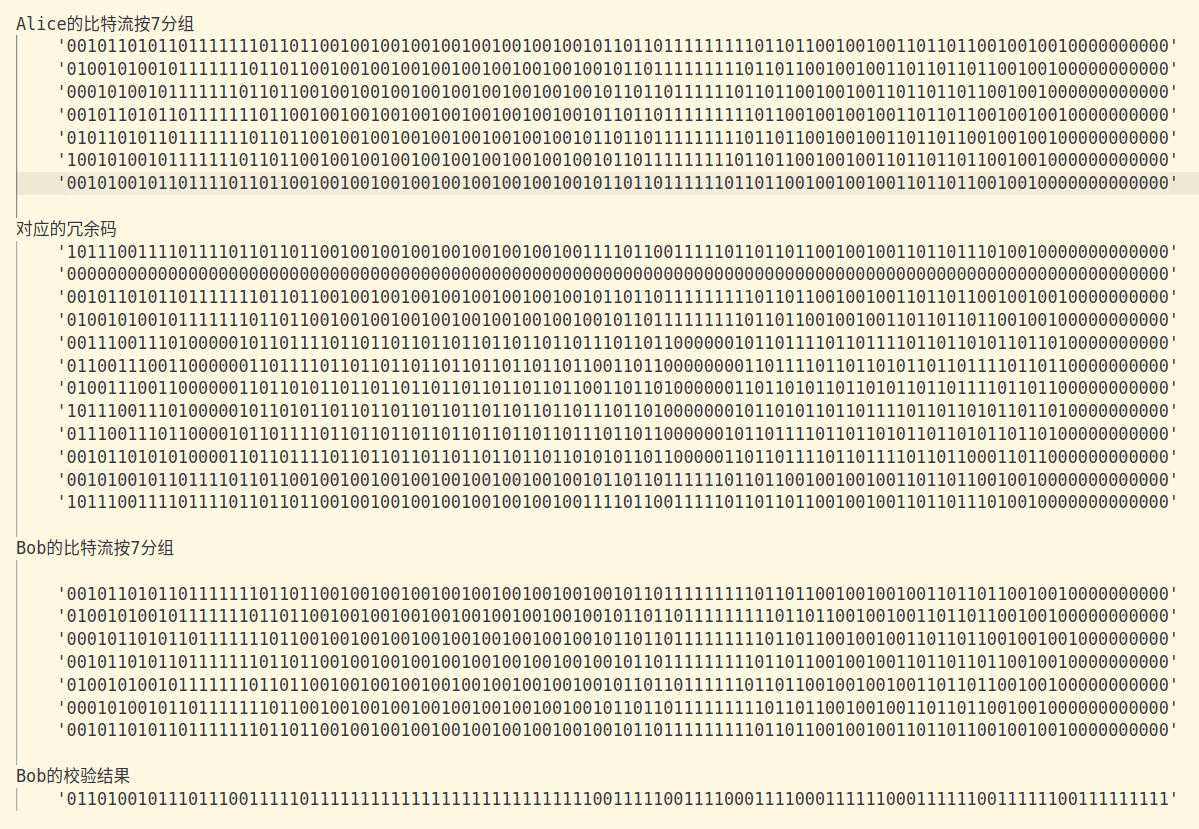
\includegraphics[width=0.9\textwidth]{images/bitstream_and_crccode} 
    \caption{CRC校验码}
    \label{bitstream_and_crccode}
\end{figure}

\subsection{基于纠错码的调和方法}

本文使用了两种纠错码,Turbo码和BCH码。首先Alice会生成随机数作为密钥,并使用Turbo码或者BCH码进行纠错编码,再异或CSI量化出的密钥比特流。之后将其发送给Bob,Bob将其和比特流异或,再进行纠错解码。除了Turbo和BCH码之外,还有LDPC码等方式。

\subsubsection{Turbo码}

Turbo码于1993年由Claude Berrou等人提出,其实现方式以时间换取逼近香农极限的性能。Turbo码的编码器和解码器如图\ref{turbo_encode}和\ref{turbo_decode}所示。Turbo码的译码算法包括MAP算法、LOG-MAP算法、Max-Log-MAP算法和SOVA算法,本文使用LOG-MAP和SOVA算法来进行译码。另外迭代次数也会影响译码算法,迭代次数越高,对信息比特的估计就越精确,但是迭代次数到达一定数值之后,译码性能改善太小。

\begin{figure}[htbp!]
    \centering 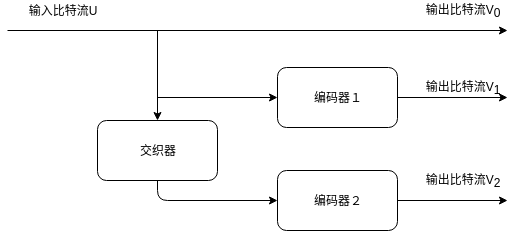
\includegraphics[width=0.9\textwidth]{images/turbo_encode} 
    \caption{Turbo编码}
    \label{turbo_encode}
\end{figure}

\begin{figure}[htbp!]
    \centering 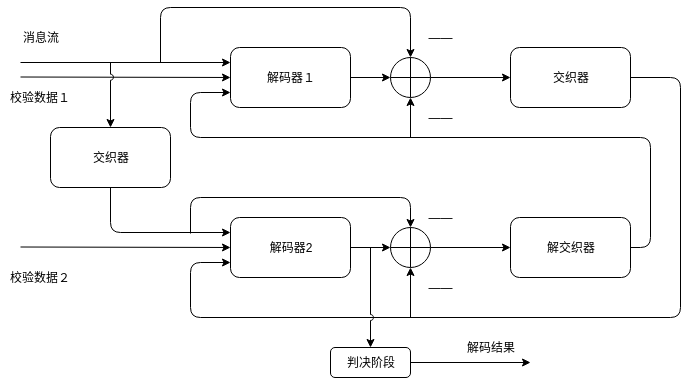
\includegraphics[width=0.9\textwidth]{images/turbo_decode} 
    \caption{Turbo解码}
    \label{turbo_decode}
\end{figure}


\subsubsection{BCH码}

BCH码(BCH codes、Bose–Chaudhuri–Hocquenghem codes)为取自Bose、Ray-Chaudhuri与Hocquenghem的缩写,是一种循环纠错码,BCH码能灵活地选择码参数,如分组长度和码率,当分组长度为几百或者更少时,BCH码被公认为同样分组长度和码率的编码中最好的码之一。

对于任意的正整数m($m \leq 3 $)和t ($ t < \frac{2^m - 1}{2} $),存在二进制BCH码满足,

\begin{table}[]
    \centering
    \begin{tabular}{|l|l|l|}
    \hline
    块长度 & $ n = 2^m - 1 $  \\ \hline
    消息比特数 & $ k \leq n - mt $  \\ \hline
    最小距离 & $ d_{min} \leq 2t + 1 $  \\ \hline
    \end{tabular}
    \caption{
    \label{}}
\end{table}

则该BCH码可以检测和纠正多达t个随机的误码。设$\alpha$为有限域$GF(2^m)$的本原根。则长度$2^m - 1$、t纠错能力的BCH码的生成多项式$g(x)$是$GF(2)$上根为$\alpha$、${\alpha}^2$、${\alpha}^3$、...、${\alpha}^{2t}$的极小多项式。设$\phi_i(x)$是$\alpha^i$的极小多项式。那么$g(x)$一定是$\phi_1(x)$、$\phi_2(x)$...$\phi_{2t}(x)$最小公倍数。即,

\begin{equation}
    g(x) = LCM\{\phi_1(x), \phi_2(x), ... , \phi_{2t}(x)\}
\end{equation}

如果i是偶数,那么可以表示成乘积形式,

\begin{equation}
    i = i'2^l
\end{equation}

其中$i'$是奇数,并且$l \leq 1$,则$\alpha^i = (\alpha^{i'})^{2^l}$是$\alpha^{i'}$的共轭,因此$\alpha^i$和$\alpha^{i'}$有相同极小多项式,因此,

\begin{equation}
    \phi_i(x) = \phi_{i'}(x)
\end{equation}

因此,$\alpha$的偶数方和$\alpha$的奇数方有相同的极小多项式,故,

\begin{equation}
    g(x) = LCM\{\phi_1(x), \phi_3(x), ... , \phi_{2t-1}(x)\}
\end{equation}

由于$ deg[\phi_i(x)] \leq m $,所以$ deg[g(x)] \leq mt $,所以 $ n -k \leq mt $。这意味着校验位的个数$n - k $最多为$mt$。当$t$非常小时,$n - k $和$mt$十分相近。

当纠错单个误码时,即汉明码。此时$g(x) = \phi_1(x)$并且$t = 1$,因为$\alpha$是$GF(2^m)$域上的本原元素,所以$\phi_1(x)$是阶数m的本原多项式,此时,

\begin{equation}
    \alpha_{2^0}, \alpha_{2^1}, \alpha_{2^2}, ..., \alpha_{2^m} = 1
\end{equation}

所以长度为$2^m - 1$、可以纠错1个误码的BCH码就是汉明码。

\section{隐私放大}

在信道探测阶段和信息调和阶段,所有交互信息对任何第三方都是可见的,这些信息中携带密钥信息,因此需要进一步进行隐私放大。通常使用哈希函数来进行隐私放大,哈希函数的单向性使得窃听者无法从公开信息中分析出密钥信息。常见的哈希函数有MD5、SHA(Secure Hash Algorithm)算法等等。本文使用SHA-2来作隐私放大,Alice和Bob将调和得到的会话密钥分别送入哈希函数,得到512比特的密钥值。

\chapter{无线密钥生成系统的实验数据分析和验证}

本文已经介绍了无线密钥生成技术的理论基础,以及无线密钥生成系统的详细设计。目前大多数研究工作专注仿真较多,本文基于GNURadio软件无线电开发平台和USRP通用软件无线电外设,设计并实现了TDD/FDD模式下的高效无线密钥生成系统,并在实际环境下测量大量数据并验证。实际测量中的信道环境更加复杂,因此本文在室内房间、室内走廊和空旷室外三种场景下的终端固定、终端移动和人员走动三种不同信道环境下多次测量数据,并根据测量结果,分析合法通信双方和窃听者CSI的互易性、CSI信息泄漏率、CSI随机性、密钥随机性、密钥生成速率、Turbo纠错码以及BCH纠错码的BER等指标来验证无线密钥生成系统的可靠性和安全性。

\section{实验平台}

本文使用GNURadio软件无线电套件开发无线密钥生成系统。其中,系统中的信道测量依赖于USRP外设发射和接收数据,特征量化、信息调和、隐私放大在PC中处理完成,信息调和的信息交互在无线局域网中完成。无线密钥生成系统可以通过配置参数实现不同频点下、不同采样率下、TDD/FDD模式的无线密钥生成,并将接收导频信号、探测结果CSI、会话密钥等中间结果转存到磁盘。

本系统使用GNURadio版本为3.7.11,使用三台USRP N210作为外设,使用三台PC部署主机程序。USRP N210可以提供高带宽、高动态范围处理能力。USRP N210拥有Xilinx® Spartan® 3A-DSP 3400 FPGA,100 MS/s的双ADC,400 Ms/s的双DAC,和PC处理器之间通过千兆以太网连接用于通信,USRP N210和主机之间的通信速度可达50 MS/s。USRP N210可以工作在0\~6GHz,并且拥有允许多个USRP N210同步构建MIMO的扩展端口。USRP N210在发射和接收方向的处理能力达到100 MS/s。

如图\ref{system-three}所示,实验中分Alice、Bob、Eve三个角色,Alice和Bob是合法通信方,Eve是窃听者。三台PC共处一个无线局域网内,因为三者之间需要通过无线局域网进行信息调和,其中Alice事先已经得知Bob和Eve的无线局域网IP。如图\ref{system-usrp}所示,每一台PC均和一台USRP N210配置在同一个有线局域网内,PC和USRP之间依靠千兆以太网网口传输数据,本系统将PC的有线局域网IP配置为$192.168.10.1$,USRP的有线局域网IP配置为$192.168.10.2$。

本文使用主从模式来实现系统流程控制,无线密钥生成系统的密钥协商过程由主端控制,从端被动响应。Alice为主端,Bob和Eve均为从端。在一次信道探测过程中,主端Alice发起信道探测,从端Bob和Eve均会探测到导频信号,Bob会回发导频信号。之后三者各自分析计算CSI并生成密钥,Alice和Bob进一步调和生成会话密钥,并用于加密信息的传输。Eve由于接收到的导频信号经过不同的信道衰落,尽管经过相同的生成步骤,但是最终生成的密钥不同,因此无法破解消息。

\begin{figure}[htbp!]
    \centering 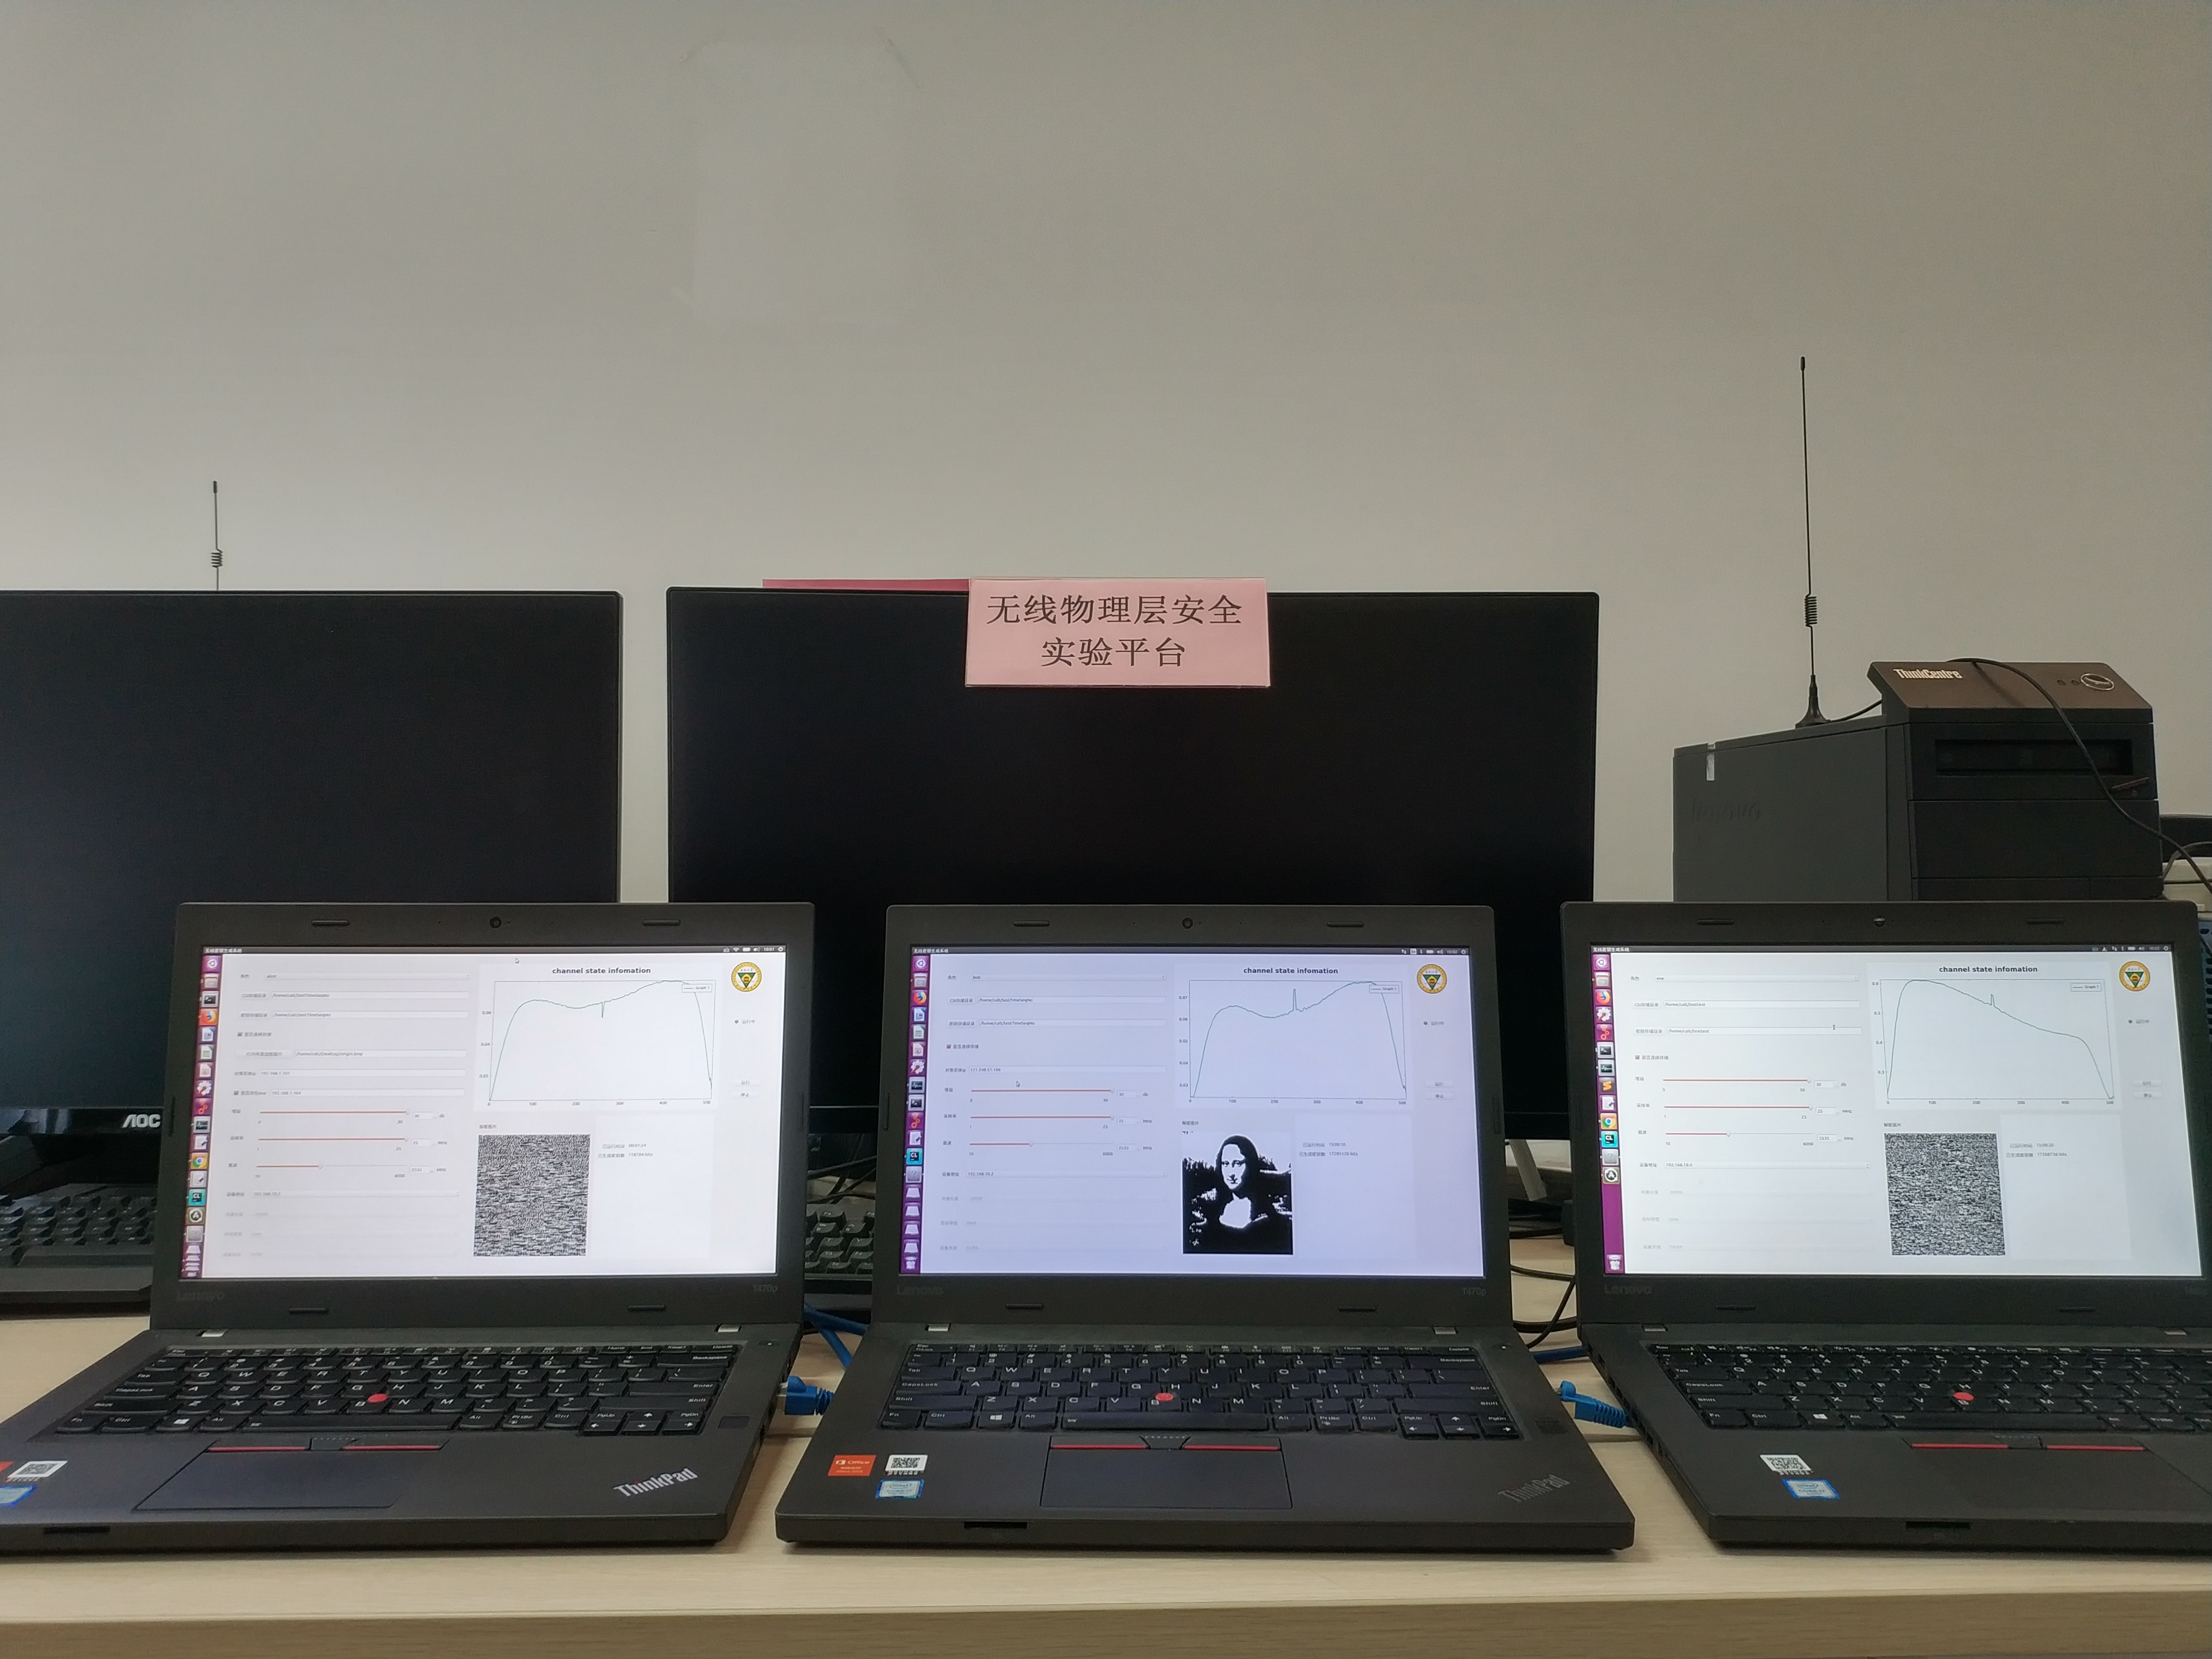
\includegraphics[width=0.9\textwidth]{images/system-three}
    \caption{无线密钥生成系统平台}
    \label{system-three}
\end{figure}

\begin{figure}[htbp!]
    \centering \includegraphics[width=0.9\textwidth]{images/system-usrp}
    \caption{PC和USRP N210}
    \label{system-usrp}
\end{figure}

如图\ref{alice}所示为无线密钥生成系统的控制界面,系统左侧为系统参数栏,系统右侧为结果显示栏。表\ref{left-column-args}为左侧参数栏说明,右侧为CSI曲线、加密后图片、系统运行时间、已生成密钥数。

\begin{figure}[htbp!]
    \centering 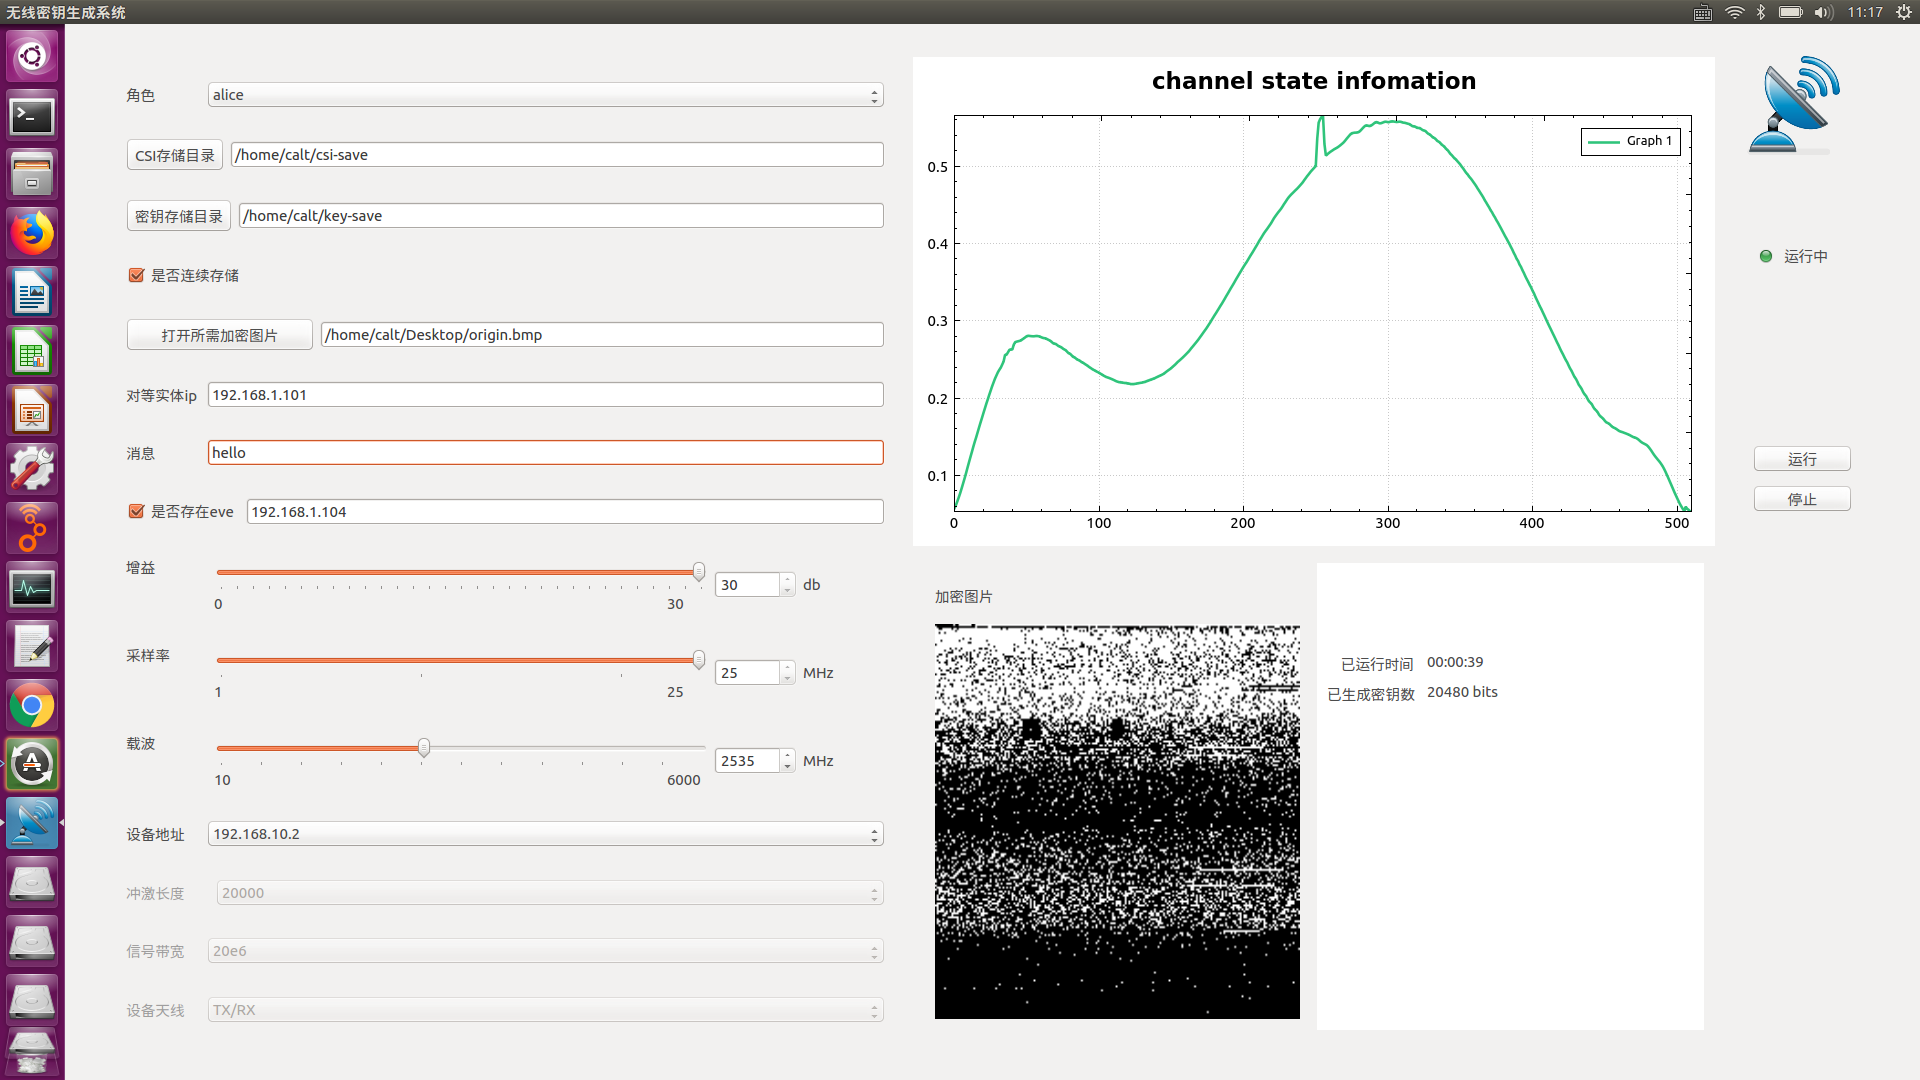
\includegraphics[width=0.9\textwidth]{images/alice}
    \caption{无线密钥生成系统的控制界面}
    \label{alice}
\end{figure}

\begin{table}[]
    \centering
    \begin{tabular}{|l|l|}
    \hline
    参数 & 说明 \\ \hline
    模式 & TDD/FDD \\ \hline
    角色 & alice/bob/eve \\ \hline
    CSI存储目录 & CSI存储位置 \\ \hline
    密钥存储目录 & 密钥存储位置 \\ \hline
    是否连续存储 & 密钥和CSI是否以追加方式存储 \\ \hline
    对等实体ip & 合法通信对方的无线局域网IP \\ \hline
    是否存在eve & 窃听方的无线局域网IP \\ \hline
    增益 & USRP增益 \\ \hline
    采样率 & USRP采样率 \\ \hline
    载波 & 载波频率 \\ \hline
    设备地址 & USRP的有线局域网IP \\ \hline
    \end{tabular}
    \caption{左侧参数说明
    \label{left-column-args}}
\end{table}
\
\section{场景架构}

本文在如图\ref{sketch_scene}所示的室内房间、室内走廊、空旷室外三种场景下使用无线密钥生成系统,并在不同场景下设计三种信道环境,

\begin{figure}
    \centering
    \subfigure[室内]{
      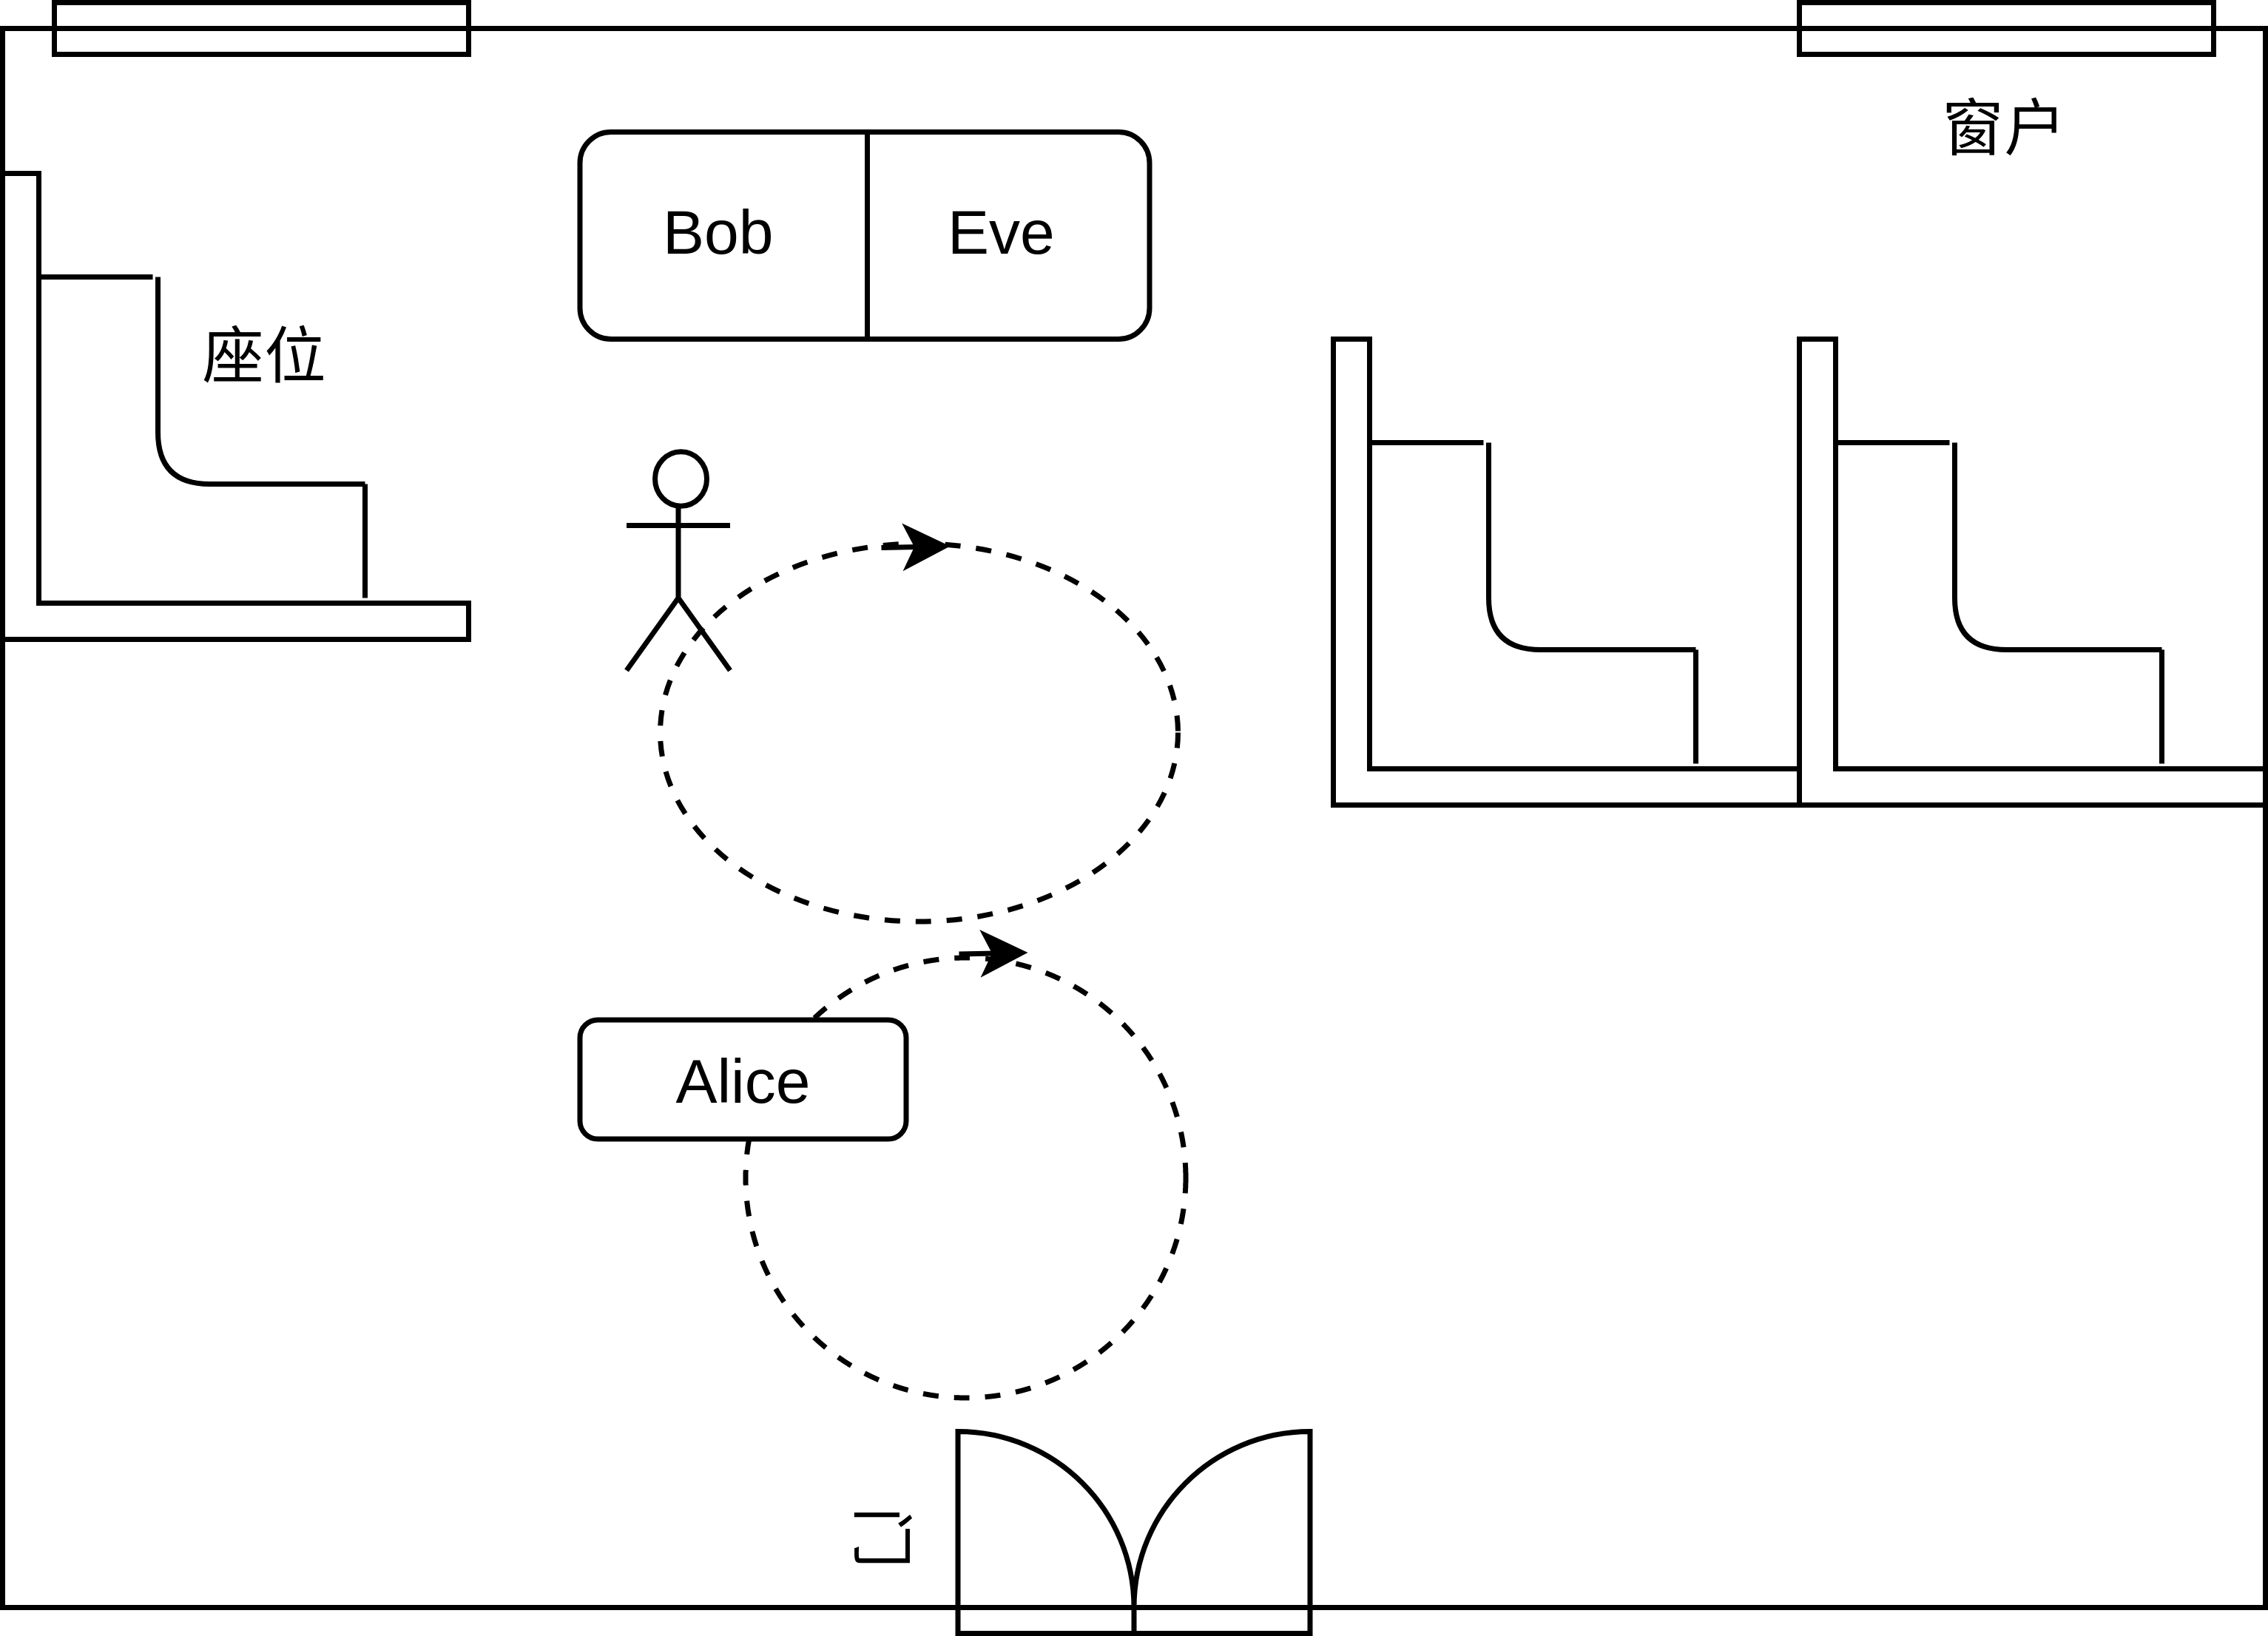
\includegraphics[width=0.9\textwidth]{images/indoor-experiment2.png}
    }
    \quad
    \subfigure[走廊]{
      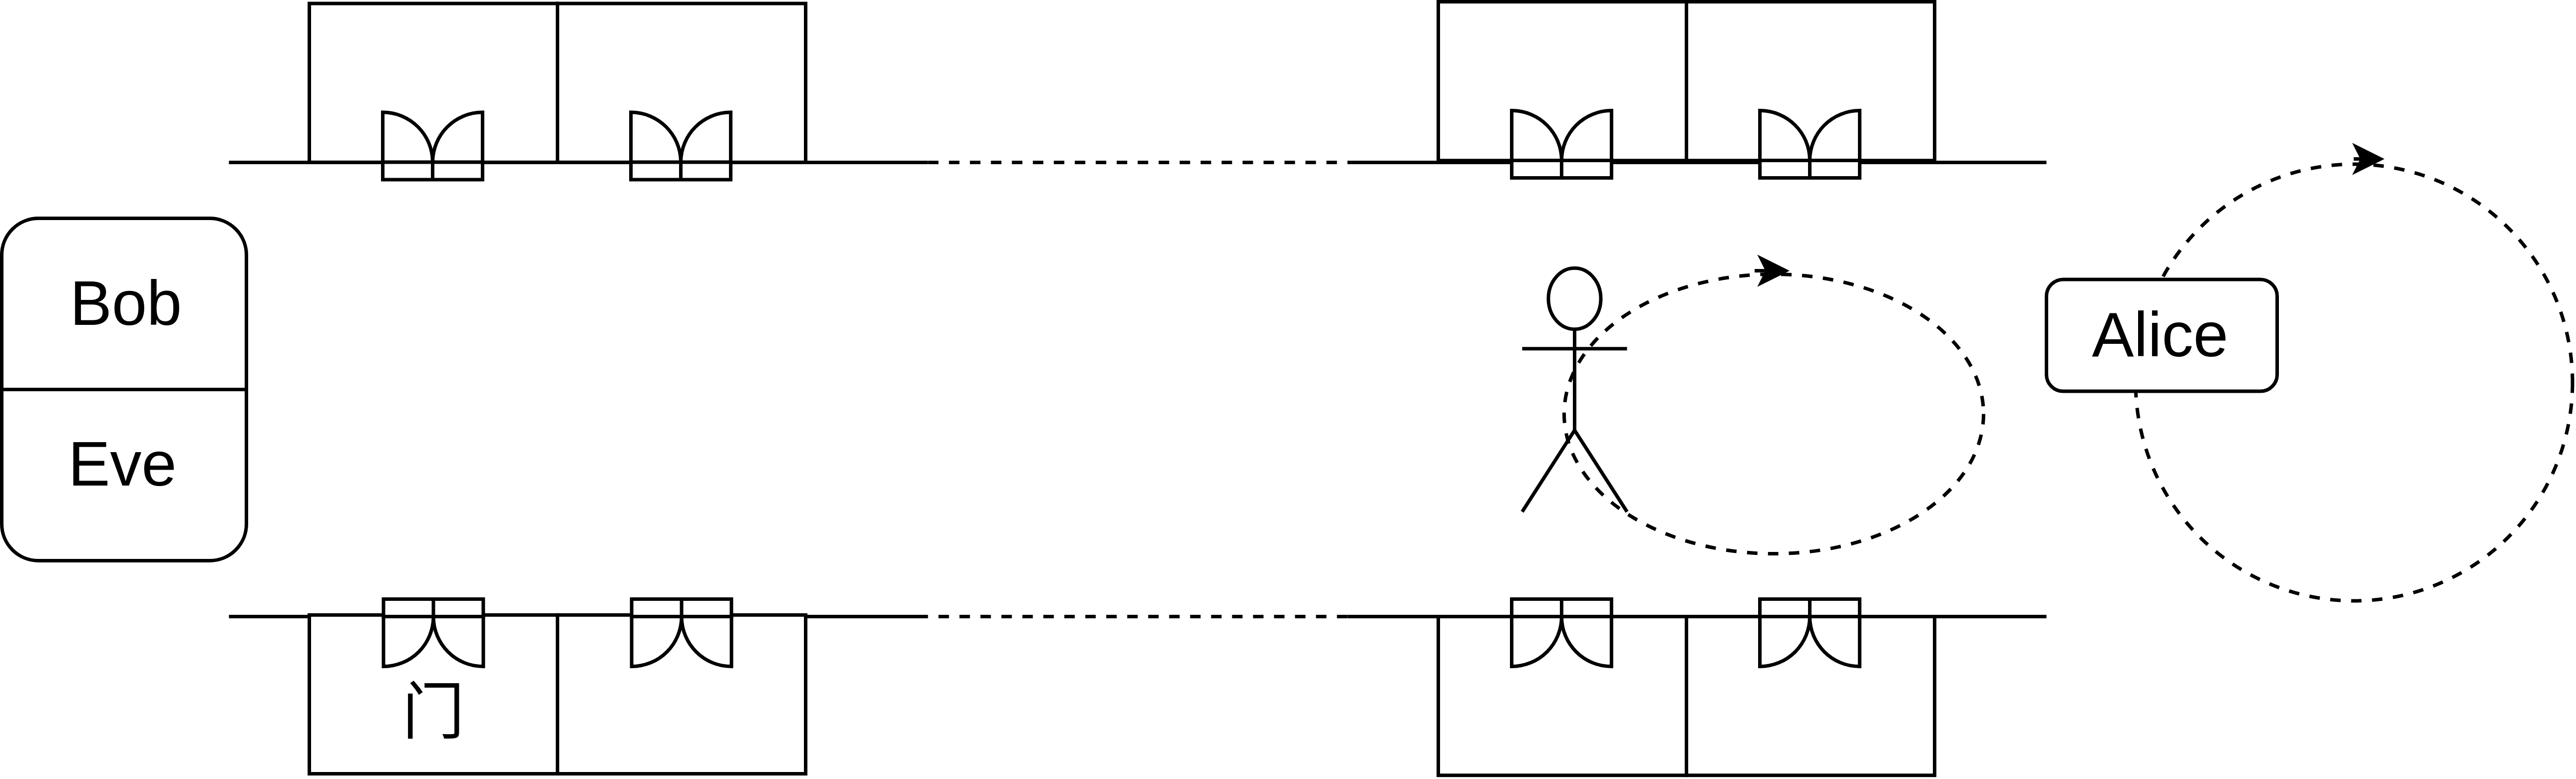
\includegraphics[width=0.9\textwidth]{images/corridor-experiment2.png}
    }
    \quad
    \subfigure[室外]{
      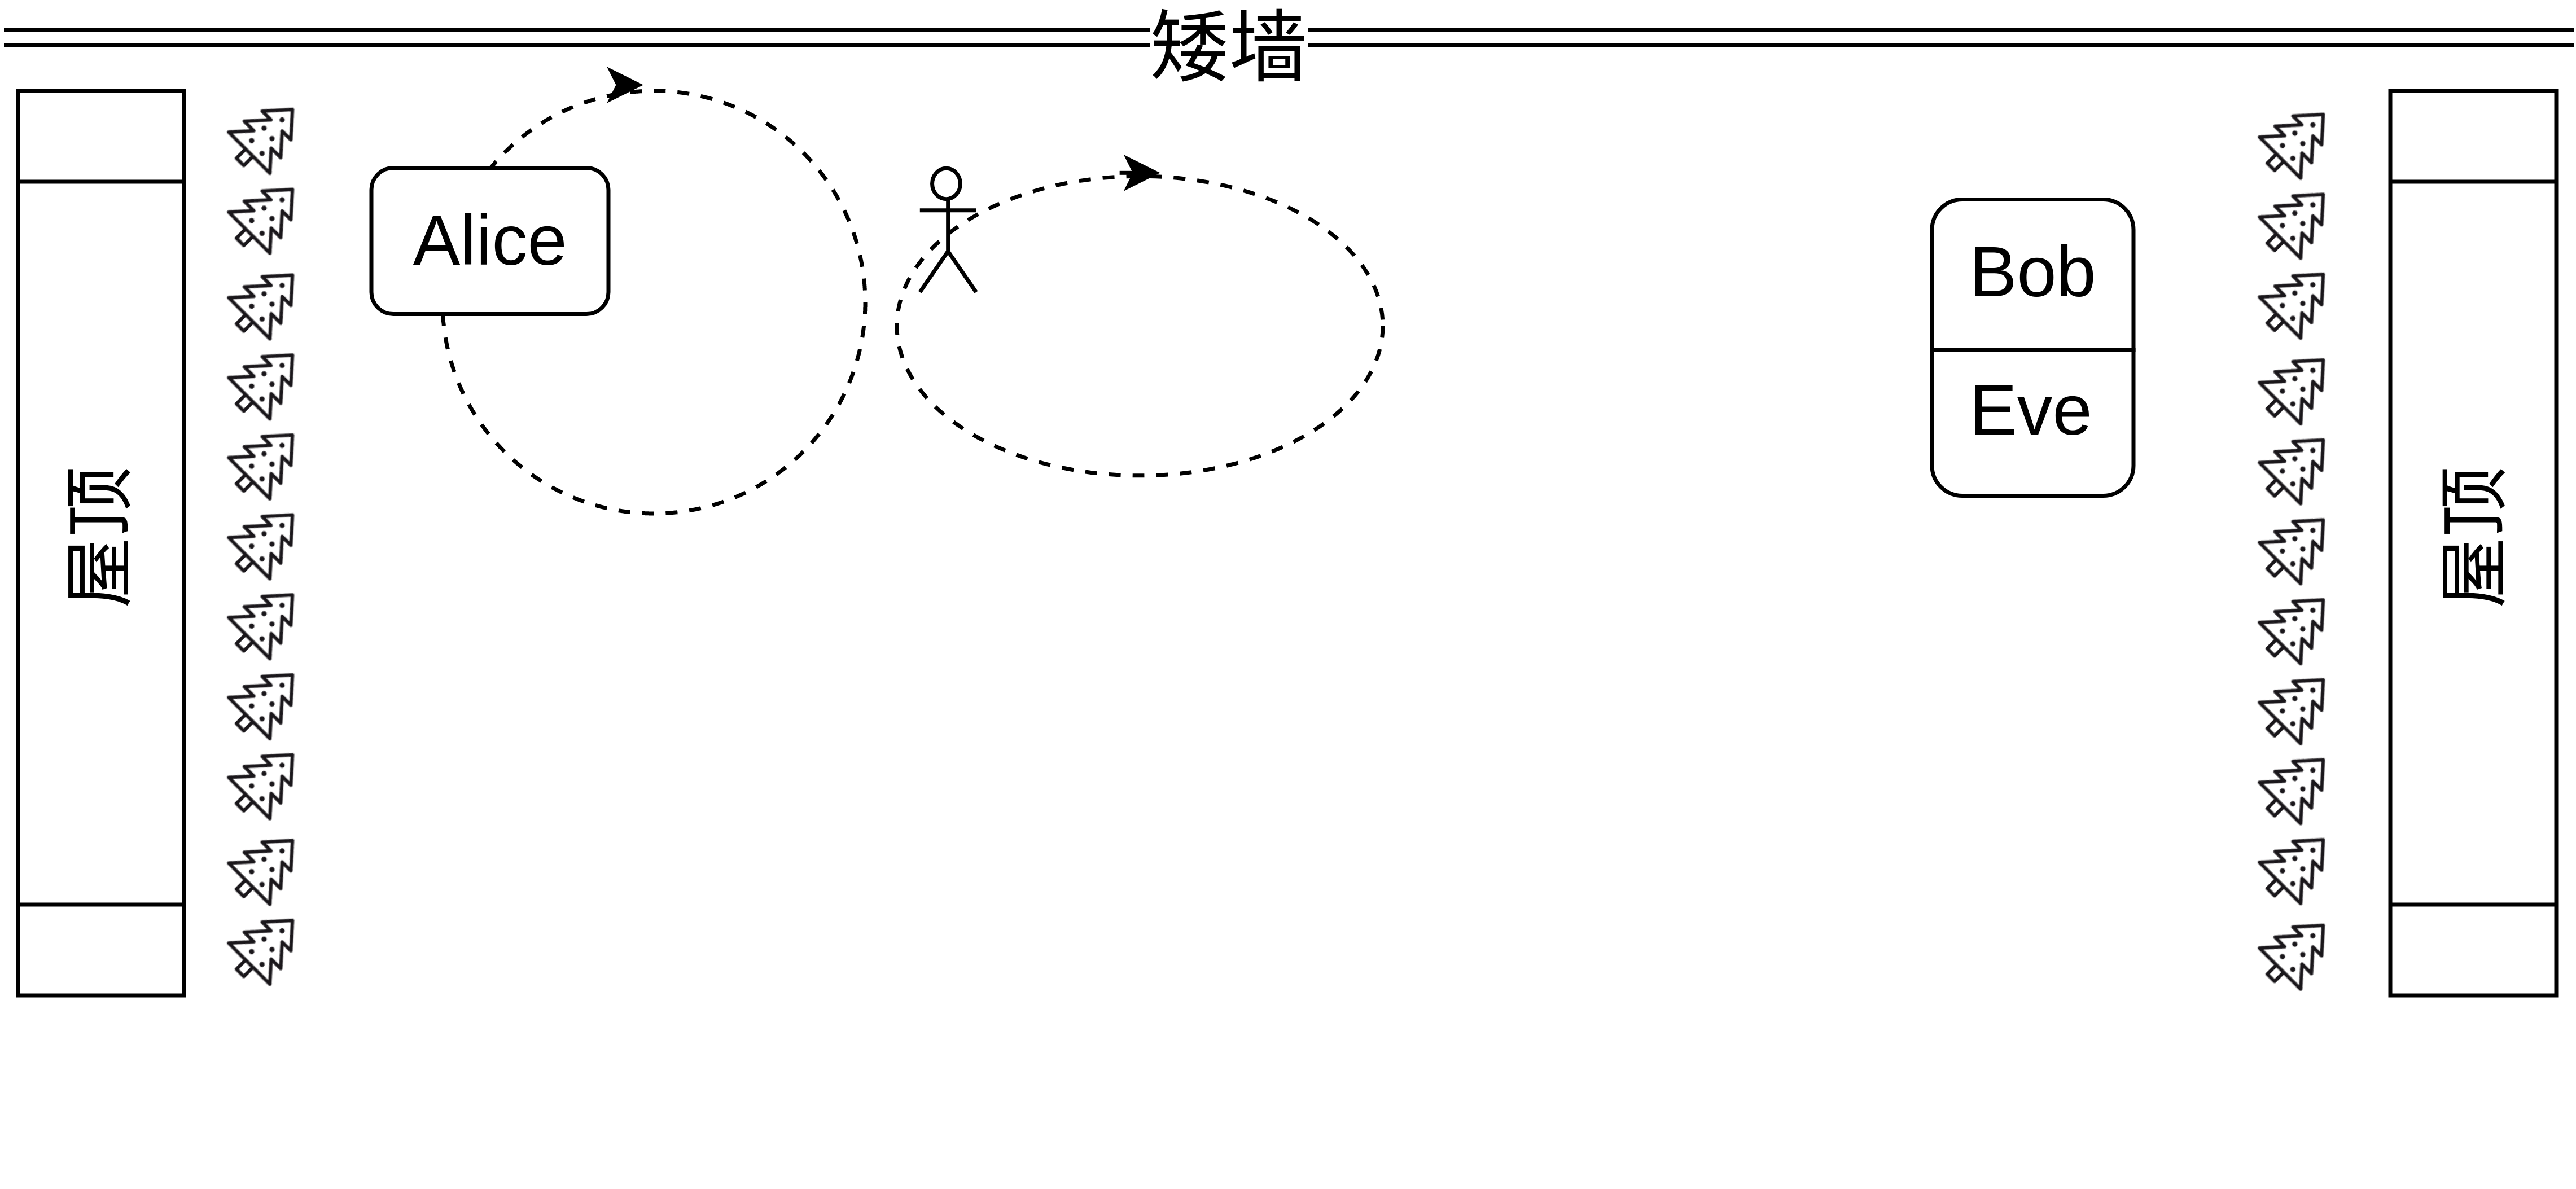
\includegraphics[width=0.9\textwidth]{images/outdoor-experiment2.png}
    }
    \quad
    \caption{室内、走廊和室外的示意图}{}
    \label{sketch_scene}
\end{figure}

\begin{itemize}
    \item \textbf{方式1} 不干扰信道
    \item \textbf{方式2} 行人在周围环境随机移动
    \item \textbf{方式3} 收发机小范围内移动   
\end{itemize}

因此本文分别在TDD和FDD模式下,测量了9种实际情况下的信道环境,并分析无线密钥生成系统的可靠性和安全性。以下将分别探讨TDD和FDD模式下,无线密钥生成系统的性能。


  
\section{TDD模式}


本文在TDD模式下的9种情况中,连续长时间采取600组数据,用于实验结果分析。TDD模式下的试验参数如表\ref{tdd-exp-args}所示,即通信方在2535MHz的频点发射和接收导频信号,导频信号前后两端设有正弦波,Alice发射的导频信号的正弦波频率为4Hz,Bob发射的导频信号的正弦波频率为8Hz,两者使用相同的、长度为4095的M序列用于精同步和信道估计,USRP的采样率均设置为25 MHz。三个场景下、三种信道环境的600组CSI如图\ref{tdd_csi_ab}所示,图中只展示了Alice的结果。图中x轴是测量次数,y轴是子载波数,z轴是幅度值,即从时间的维度来观察CSI的变化。

对比9种场景下的CSI变化,可以看出,室内静态环境下的CSI几乎不变,因为室内信道环境干扰较少,因此信道变化缓慢。与室内静态环境相反的是室外方式三和走廊方式三,这两种情况下CSI变化十分剧烈,一方面终端一直在移动导致的多普勒效应,另一方面室内走廊和空旷室外的信道环境干扰较多。显然,在所有信道环境中,终端完全固定的信道环境下,CSI变化最为平缓;终端移动的信道环境下,CSI变化最为剧烈。在所有场景中,室内房间场景下测量的CSI变化最为平缓,空旷室外场景下测量的CSI变化最为剧烈。CSI变化越剧烈,则每次探测生成的密钥越随机,同时说明信道变化越剧烈,这可能会带来密钥生成速率的降低,因为信道变化剧烈会影响通信双方的互易性。从9种场景的CSI对比可以看出,多普勒频移和较为复杂的信道环境会带来信道的剧烈改变,进而影响CSI的快速变化。

本文接下来将通过计算多个指标,分析无线密钥生成系统的可靠性和安全性。

\begin{figure}
    \centering
    \subfigure[室内-方式1]{
        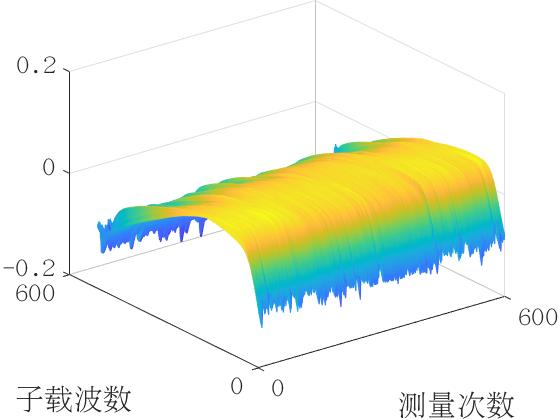
\includegraphics[width=0.3\textwidth]{images/tdd-csi/indoor-no-move.jpg}
    }
    \subfigure[室内-方式2]{
        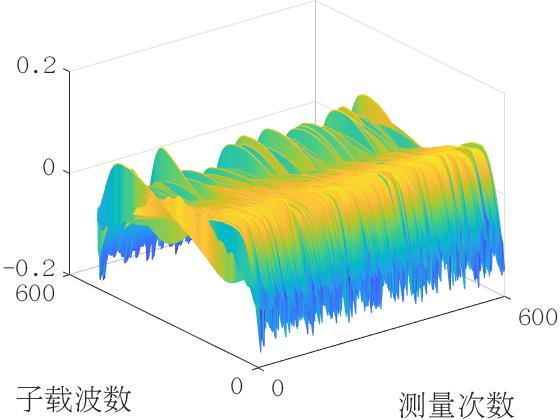
\includegraphics[width=0.3\textwidth]{images/tdd-csi/indoor-people-move.jpg}
    }
    \subfigure[室内-方式3]{
        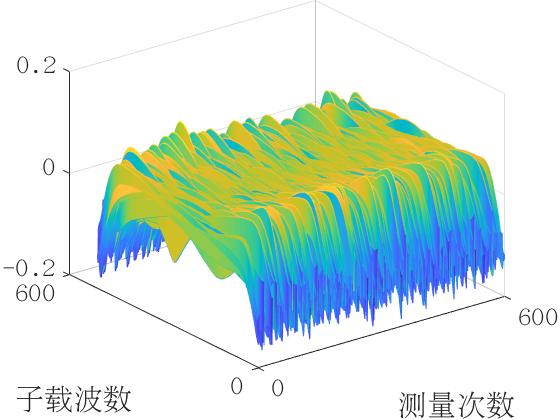
\includegraphics[width=0.3\textwidth]{images/tdd-csi/indoor-trolly-move.jpg}
    }
    \quad    %用 \quad 来换行
    \subfigure[走廊-方式1]{
        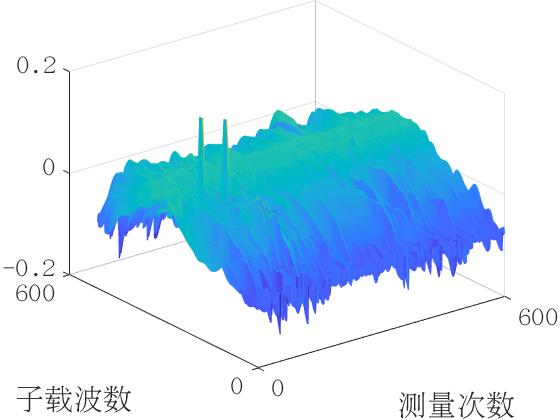
\includegraphics[width=0.3\textwidth]{images/tdd-csi/corridor-no-move.jpg}
    }
    \subfigure[走廊-方式2]{
        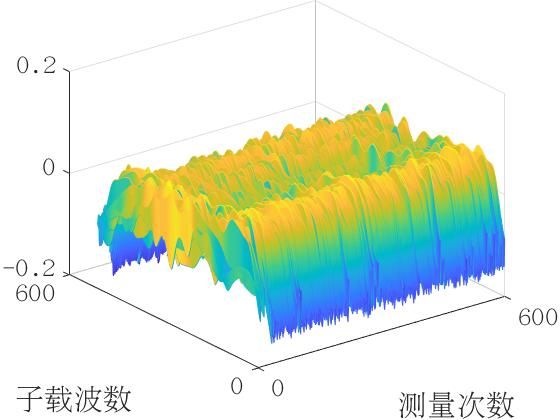
\includegraphics[width=0.3\textwidth]{images/tdd-csi/corridor-people-move.jpg}
    }
    \subfigure[走廊-方式3]{
        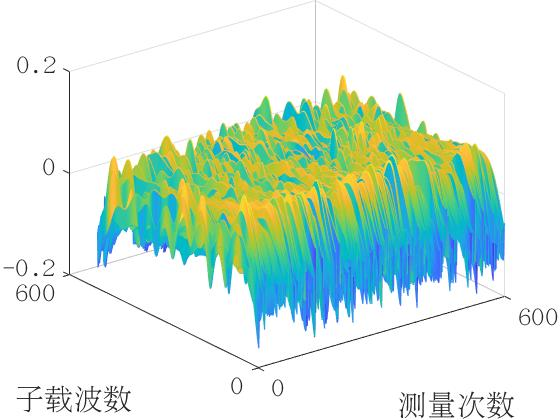
\includegraphics[width=0.3\textwidth]{images/tdd-csi/corridor-trolly-move.jpg}
    }
    \quad
    \subfigure[室外-方式1]{
        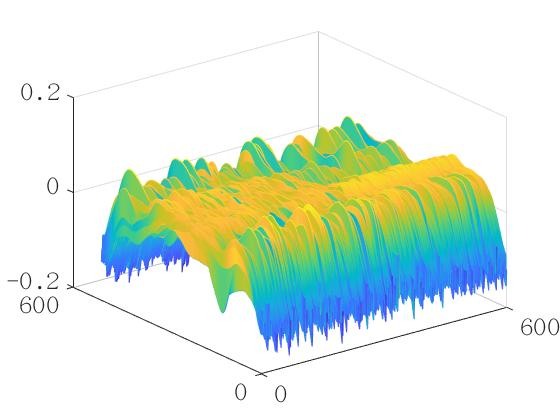
\includegraphics[width=0.3\textwidth]{images/tdd-csi/outdoor-no-move.jpg}
    }
    \subfigure[室外-方式2]{
        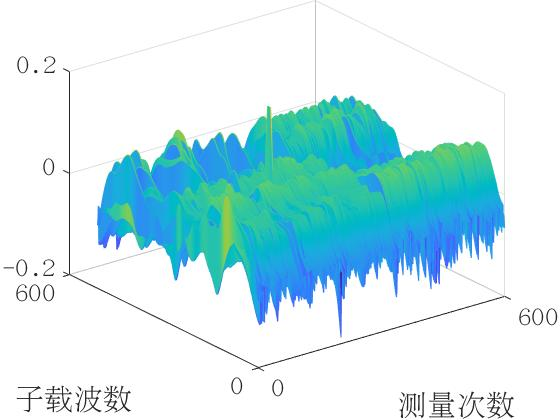
\includegraphics[width=0.3\textwidth]{images/tdd-csi/outdoor-people-move.jpg}
    }
    \subfigure[室外-方式3]{
        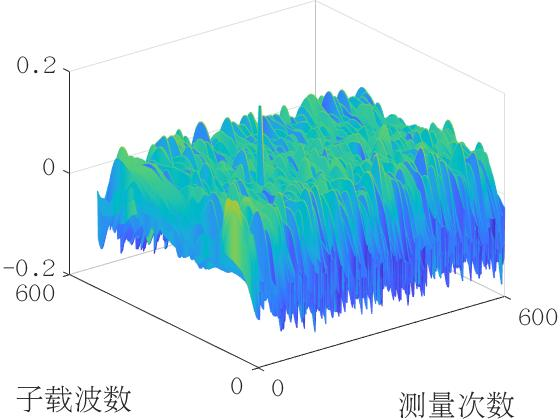
\includegraphics[width=0.3\textwidth]{images/tdd-csi/outdoor-trolly-move.jpg}
    }
    \caption{不同场景与环境下CSI结果展示}{} % xcorr between alice and bob, xcorr between bob and eve
    \label{tdd_csi_ab}
\end{figure}

% Please add the following required packages to your document preamble:
% \usepackage{multirow}
\begin{table}[]
    \centering
    \begin{tabular}{|l|l|l|l|}
    \hline
    \multicolumn{2}{|c|}{参数} & Alice & Bob \\ \hline
    \multirow{5}{*}{USRP} & 上下行载波频率(MHz) & 2535 & 2535 \\ \cline{2-4} 
     & 采样率(MHz) & 25 & 25 \\ \cline{2-4} 
     & 增益(dB) & 30 & 30 \\ \cline{2-4} 
     & 天线 & Tx/Rx & Tx/Rx \\ \cline{2-4} 
     & 带宽(MHz) & 20 & 20 \\ \hline
    \multirow{4}{*}{导频信号} & 正弦波长度 & 1504 & 1504 \\ \cline{2-4} 
     & 正弦波频率(Hz) & 4 & 8 \\ \cline{2-4} 
     & M序列长度 & 4095 & 4095 \\ \cline{2-4} 
     & CP循环前缀长度 & 129 & 129 \\ \hline
    \end{tabular}
    \caption{TDD模式下的实验参数
    \label{tdd-exp-args}}
\end{table}

\subsection{CSI相关性}

本文对每一组数据使用公式(\ref{equation_corr_ab})和公式(\ref{equation_corr_ae})分别计算Alice和Bob之间CSI的皮尔逊相关系数、Alice和Eve之间CSI的皮尔逊相关系数。在9种情况下,计算600组数据,得到图\ref{tdd_csi_xcorr}。其中蓝色表示Alice和Bob之间CSI的皮尔逊相关系数,红色表示Alice和Eve之间CSI的皮尔逊相关系数。可以看到Alice和Bob之间CSI的相关系数稳定在1附近,Alice和Eve之间CSI的相关系数波动较大并且较小。

\begin{figure}
    \centering
    \subfigure[室内-方式1]{
        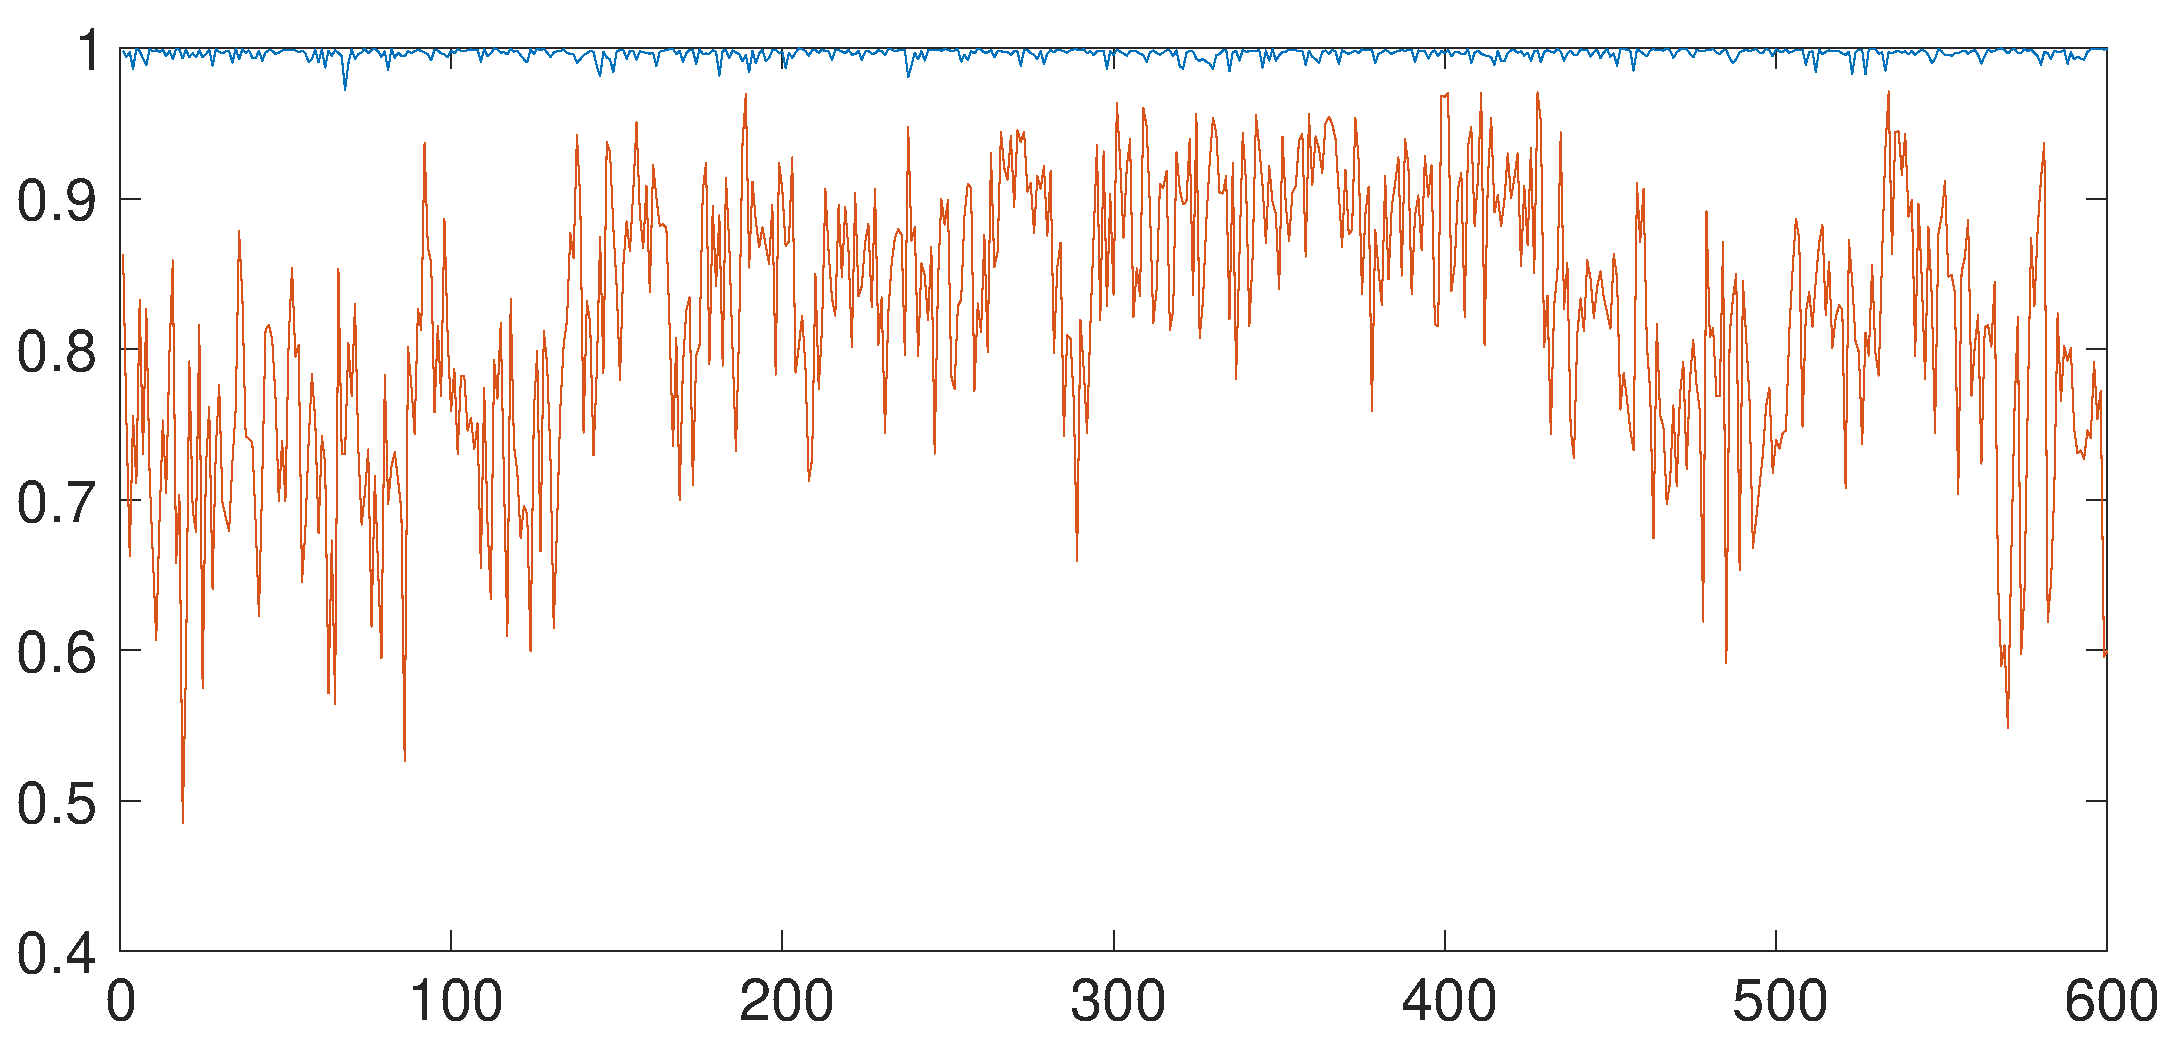
\includegraphics[width=0.3\textwidth]{images/tdd-xcorr/indoor-no-move.eps}
    }
    \subfigure[室内-方式2]{
        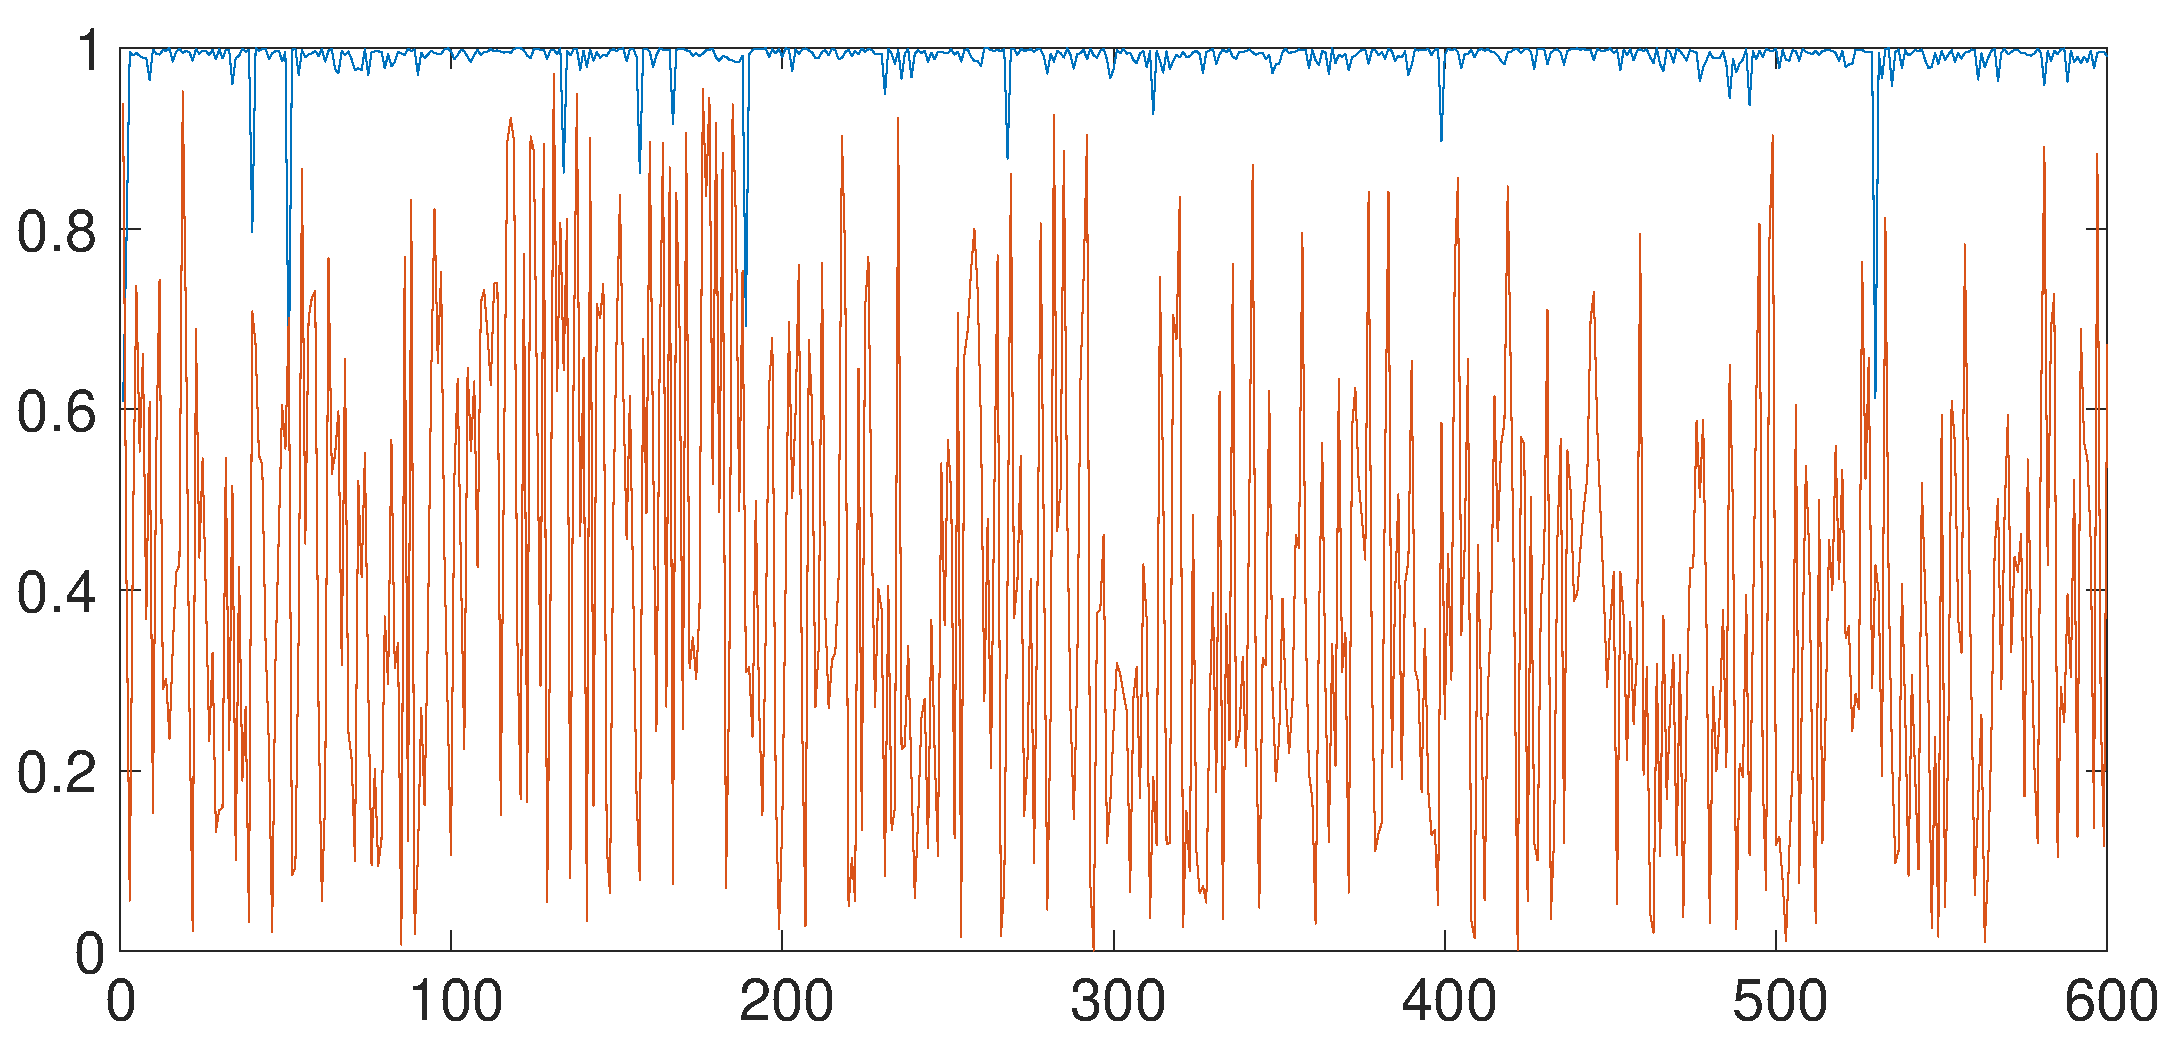
\includegraphics[width=0.3\textwidth]{images/tdd-xcorr/indoor-people-move.eps}
    }
    \subfigure[室内-方式3]{
        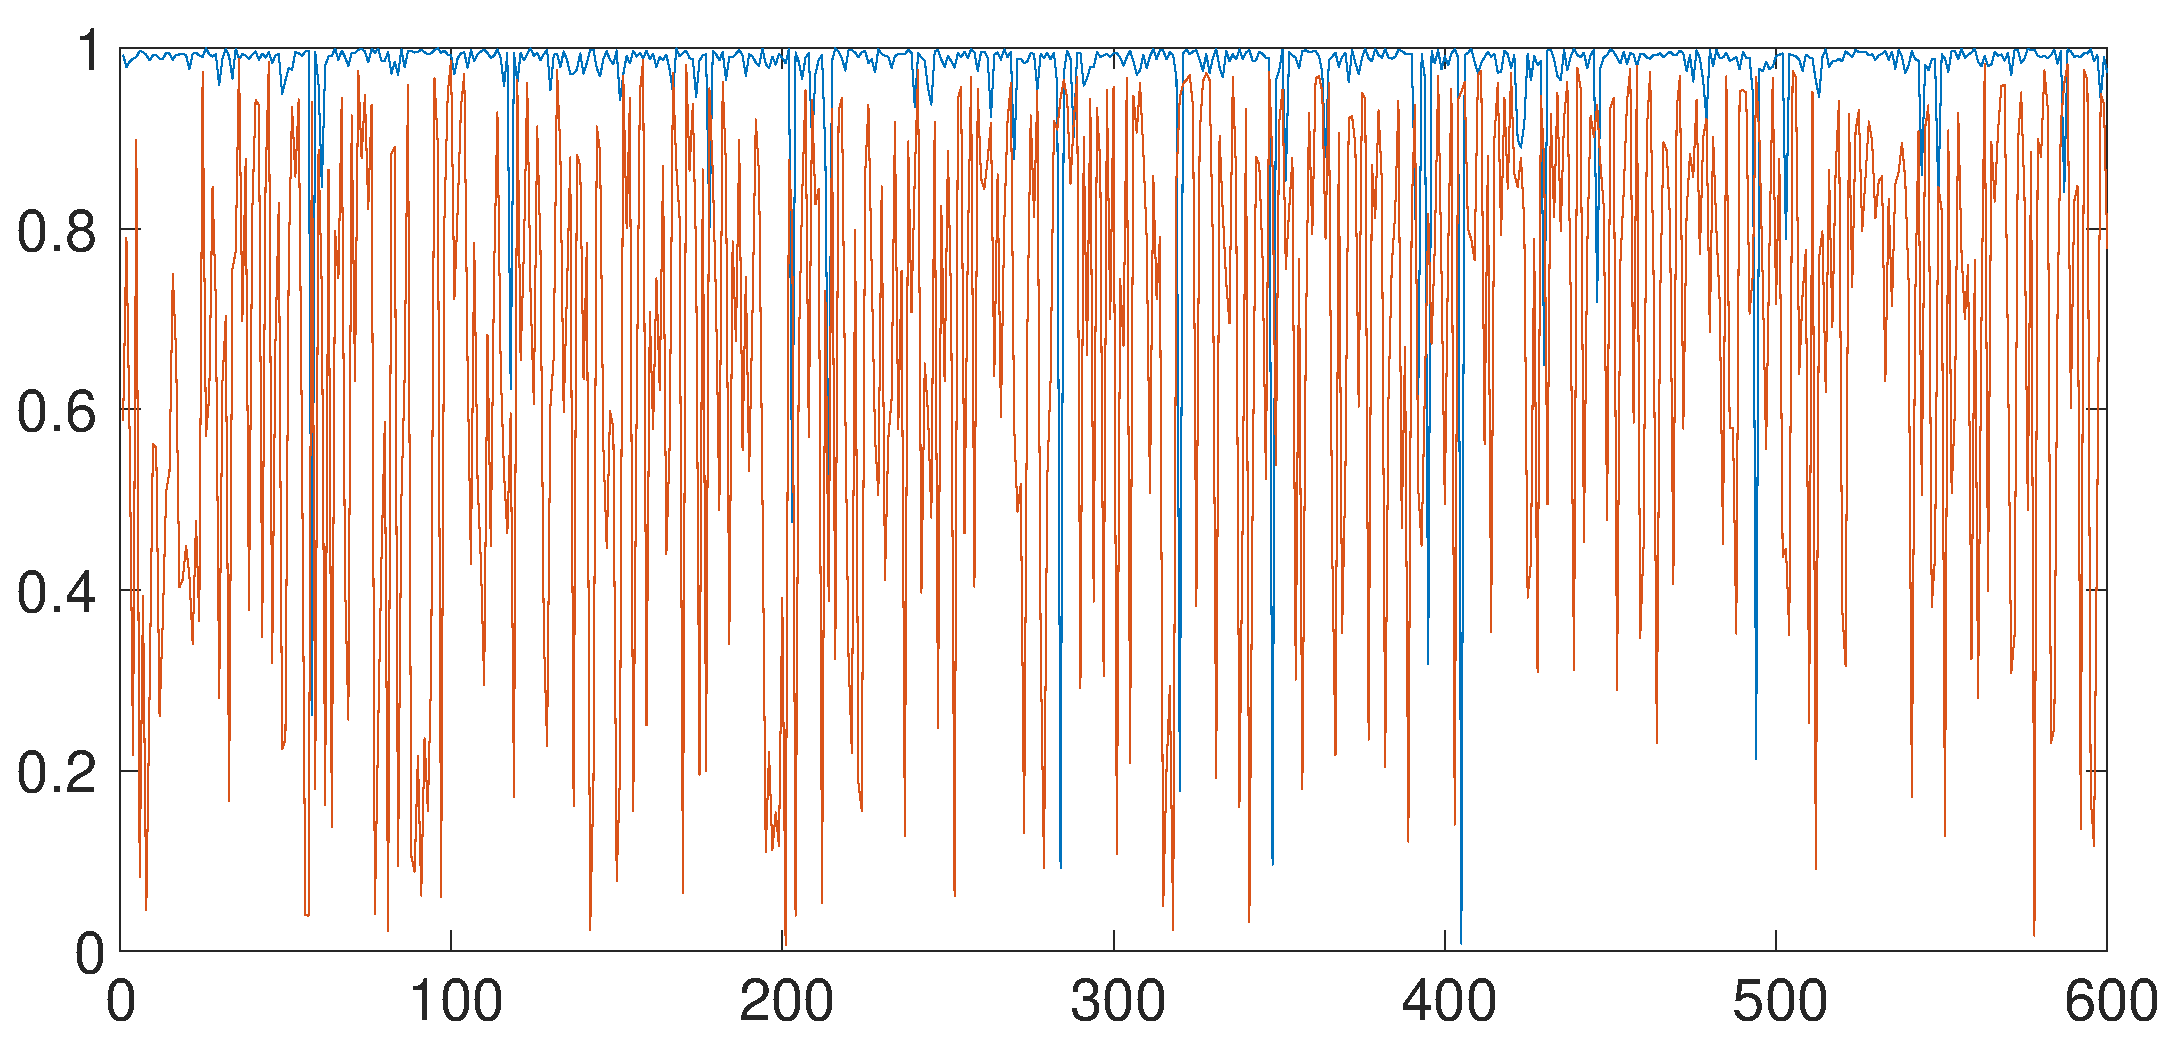
\includegraphics[width=0.3\textwidth]{images/tdd-xcorr/indoor-trolly-move.eps}
    }
    \quad    %用 \quad 来换行
    \subfigure[走廊-方式1]{
        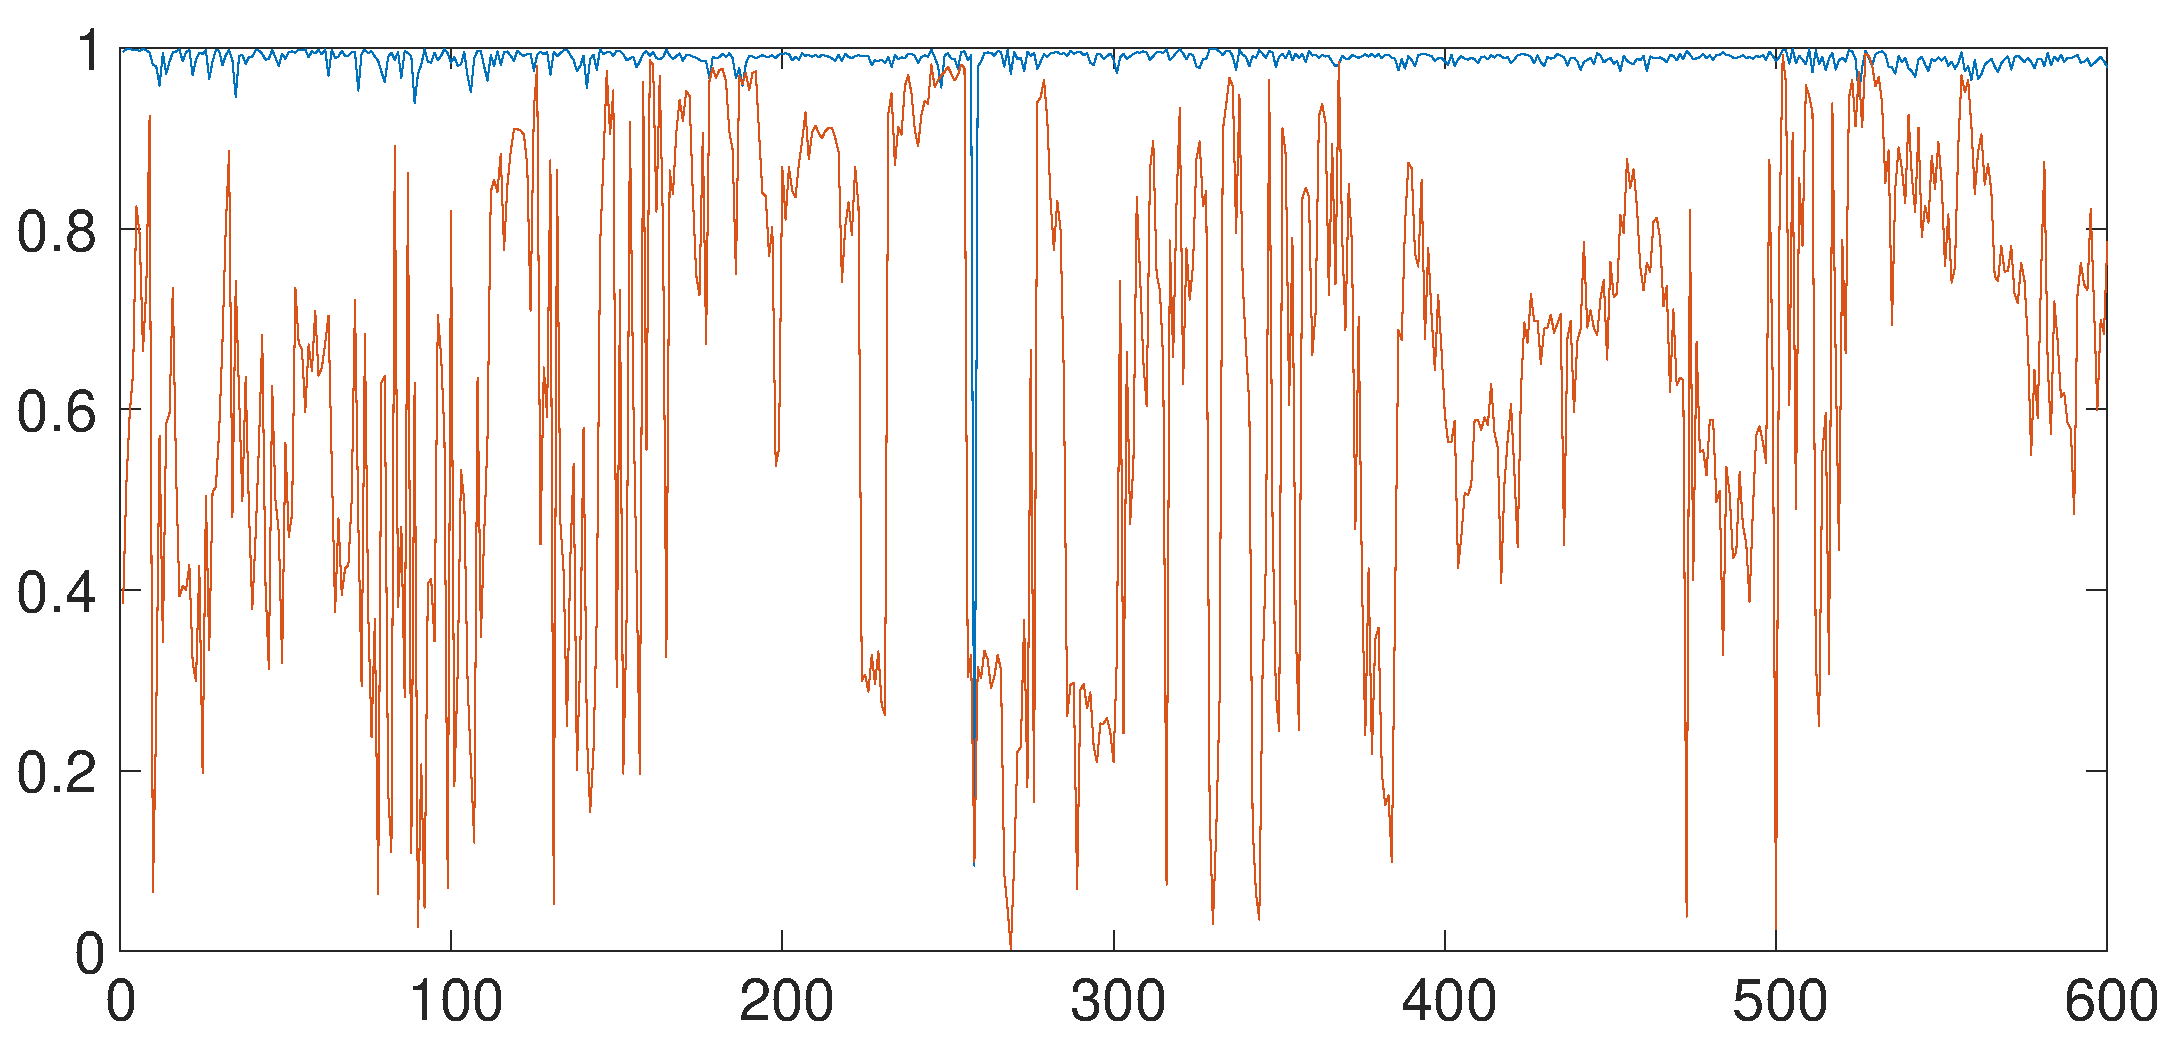
\includegraphics[width=0.3\textwidth]{images/tdd-xcorr/corridor-no-move.eps}
    }
    \subfigure[走廊-方式2]{
        \includegraphics[width=0.3\textwidth]{images/tdd-xcorr/corridor-people-move.eps}
    }
    \subfigure[走廊-方式3]{
        \includegraphics[width=0.3\textwidth]{images/tdd-xcorr/corridor-trolly-move.eps}
    }
    \quad
    \subfigure[室外-方式1]{
        \includegraphics[width=0.3\textwidth]{images/tdd-xcorr/outdoor-no-move.eps}
    }
    \subfigure[室外-方式2]{
        \includegraphics[width=0.3\textwidth]{images/tdd-xcorr/outdoor-people-move.eps}
    }
    \subfigure[室外-方式3]{
        \includegraphics[width=0.3\textwidth]{images/tdd-xcorr/outdoor-trolly-move.eps}
    }
    \caption{不同场景与环境下Alice和Bob、Alice和Eve之间CSI相关系数}{} % xcorr between alice and bob, xcorr between bob and eve
    \label{tdd_csi_xcorr}
\end{figure}

将多组数据取平均,得到9种情况下,Alice、Bob和Eve之间的平均皮尔逊相关系数如图\ref{tdd_bar_xcorr}所示。分析结果表明,在9种情况下,Alice与Bob之间相关性均远高于Alice与Eve。无论哪种情况,Alice和Bob之间相关系数均高于0.9711,该情况出现在室内终端移动的情况下,Alice和Bob之间相关系数最高出现在室内房间终端固定的情况下,高达0.9963。而Alice与Eve之间相关系数最高也只有0.8192,并且出现在室内房间终端固定的情况下。无论是室内、走廊还是室外,当有人员在周围环境走动时,Alice与Eve之间的信道相关性最低,其中室内终端移动情况下低至0.4004。

\begin{figure}[htbp!]
    \centering \includegraphics[width=0.9\textwidth]{images/tdd-xcorr/bar2.eps}
    \caption{不同场景下三者之间的互相关系数柱状图}
    \label{tdd_bar_xcorr}
\end{figure}

\subsection{信息泄漏率}

虽然第三方在无线密钥生成过程中通过相同生成步骤得到相同的会话密钥,但是对无线密钥生成的所有过程对于第三方来说都是完全透明的\cite{sahin2016secure},第三方可以在信道探测过程探测导频信号、在信息调和过程中窃听调和信息,因此本文通过信息论中未泄露的信息量来评估系统的安全性。

本文在9种情况下按照公式(\ref{safe_rate_equation})计算了多组安全信息率并取平均,9种情况下的平均安全信息率如图\ref{tdd_bar_leak}所示。从图中可知,无论是室内、走廊还是室外,均是当有人员在周围环境走动时安全信息率最高,其中在室外,信息安全比率高达91.01\%,这也是所有情况中的最高值,在走廊,信息安全比率为78.52\%。在所有情况中,室内房间终端移动时的信息安全比率最低,低至67.05\%。9种情况的平均安全信息率具体数据为表\ref{tdd_bar_leak_data}。


\begin{figure}[htbp!]
    \centering \includegraphics[width=0.9\textwidth]{images/tdd-leak/bar.eps}
    \caption{不同场景下的平均安全信息率柱状图}
    \label{tdd_bar_leak}
\end{figure}

% \begin{table}[!ht]
%     \centering
%     \begin{tabular*}{\hsize}{@{}@{\extracolsep{\fill}}|c|c|c|c|@{}}
%     \toprule
%         & \textbf{方式1} & \textbf{方式2} & \textbf{方式3} \\
%     \midrule
%     室内 & 0.7962 & 0.8924 & 0.6705 \\ 
% 	走廊 & 0.7604 & 0.7852 & 0.7725 \\ 
%     室外 & 0.8177 & 0.9101 & 0.7882 \\
%     \bottomrule
%     \end{tabular*}
%     \caption{不同场景下的平均安全信息率数值
%     \label{tdd_bar_leak_data}}
% \end{table}

\begin{table}[htbp] % 依赖包 booktabs
    \centering
    \setlength{\tabcolsep}{16mm}{
    \begin{tabular}{cccc}
    \toprule
        & \textbf{方式1} & \textbf{方式2} & \textbf{方式3} \\
    \midrule
    室内 & 0.7962 & 0.8924 & 0.6705 \\ 
	走廊 & 0.7604 & 0.7852 & 0.7725 \\ 
    室外 & 0.8177 & 0.9101 & 0.7882 \\
    \bottomrule
    \end{tabular}
    }
    \caption{不同场景下的平均安全信息率数值
    \label{tdd_bar_leak_data}}
\end{table}


本文计算出室内、走廊、室外三种场景下,所有信道环境下的安全信息率平均值,如表\ref{three_scene_avg}所示。表中结果说明各种信道环境下,室外的信息安全比率最高,高达83.87\%,走廊的信息安全比率最低,低至77.27\%。也计算出终端固定、人员移动、终端移动三种信道环境下,所有场景的安全信息率平均值,如表\ref{three_channel_env_avg}。表中说,各种场景下,人员移动的安全比率最高,高达86.26\%,终端移动的安全比率最低,低至74.37\%。从结果中可以看出,信道适当的变化可以提高无线密钥生成系统的信息安全比率。室内和走廊的平均值相近,说明室内和走廊场景对安全信息比率影响相似,室外场景会提高安全信息比率。相对于终端固定和终端移动的信道环境,人员移动对信息安全比率有很大的改善。


\begin{table}[]
    \centering
    \setlength{\tabcolsep}{22mm}{
    \begin{tabular}{ccc}
    \toprule
    室内 & 走廊 & 室外 \\ 
    \midrule
    78.64\% & 77.27\% & 83.87\% \\ 
    \bottomrule
    \end{tabular}
    }
    \caption{室内、走廊和室外三种场景的平均安全信息率
    \label{three_scene_avg}}
\end{table}

\begin{table}[]
    \centering
    \setlength{\tabcolsep}{20mm}{
    \begin{tabular}{ccc}
    \toprule
    终端固定 & 人员移动 & 终端移动 \\
    \midrule
    79.14\% & 86.26\% & 74.37\% \\ 
    \bottomrule
    \end{tabular}
    }
    \caption{终端固定、人员走动和终端移动三种信道环境的平均安全信息率
    \label{three_channel_env_avg}}
\end{table}

\subsection{随机性评估}

本文使用两种指标来作系统的随机性评估,使用频域的图像熵以及NIST随机性测试分别评估CSI随机性和密钥随机性。

\subsubsection{CSI随机性}

本文在理论基础部分提出了用图像熵评估CSI随机性的理论依据,CSI的图像熵展示了时域以及频域的变化。为了更好的对比,本文计算了信道无多径且不随时间变化、信道有多径且不随时间变化、信道随时间不同完全随机变化三种特殊情况下的CSI作为对比,其CSI如图\ref{special_csi}所示,三种特殊情况对应熵值如表\ref{entropy_spectial}所示。信道完全无多径且不变化时,图像熵接近于0,信道有多径且不随时间变化时稍大,但也接近于0。当信道随时间不同完全随机的情况下,图像熵为7.0098。因此本文测量数据计算出的CSI图像熵应该出现在0.00006~7.0098之间。

\begin{figure}
    \centering
    \subfigure[信道无多径且不随时间变化]{
      \includegraphics[width=0.3\textwidth]{images/spectial-entropy/constant.eps}
    }
    \subfigure[信道有多径且不随时间变化]{
      \includegraphics[width=0.3\textwidth]{images/spectial-entropy/multipath.eps}
    }
    \subfigure[信道随时间不同完全随机变化]{
      \includegraphics[width=0.3\textwidth]{images/spectial-entropy/random.eps}
    }
    \caption{特殊情况下CSI结果展示}{} % xcorr between alice and bob, xcorr between bob and eve
    \label{special_csi}
\end{figure}

\begin{table}[]
    \centering
    \setlength{\tabcolsep}{4mm}{
    \begin{tabular}{ccc}
        \toprule
        \textbf{信道无多径且不随时间变化} & \textbf{信道有多径且不随时间变化} & \textbf{信道随时间不同完全随机变化} \\
        \midrule
        0.00006 & 0.0262 & 7.0098 \\
        \bottomrule
    \end{tabular}
    }
    \caption{特殊情况的图像熵值
    \label{entropy_spectial}}
\end{table}

\begin{table}[]
    \centering
    \setlength{\tabcolsep}{16mm}{
    \begin{tabular}{cccc} 
        \toprule
        & \textbf{方式1} & \textbf{方式2} & \textbf{方式3} \\
        \midrule
        室内 & 2.5391 & 3.7227 & 3.9960 \\ 
        走廊 & 3.3293 & 3.8674 & 4.0667 \\ 
        室外 & 3.8696 & 3.8933 & 4.0924 \\
        \bottomrule
    \end{tabular}
    }
    \caption{不同场景的图像熵值
    \label{entropy_fft2d}}
\end{table}

本文在每个情况下,使用600组CSI按照公式(\ref{entropy_fft2d_equation})计算多组CSI的图像熵,如表\ref{entropy_fft2d}。从表中可以看出,无论哪种信道环境,室内房间的CSI随机性均最低,空旷室外的CSI随机性最高。无论哪种场景,终端固定的信道环境下的CSI随机性最低,终端移动的信道环境下的CSI随机性最高。所有情况中,在室内场景下的终端固定时CSI随机性最低,低至2.5391;在室外场景下的终端移动时CSI随机性最高,高达4.0924。从表中分析得知,随着信道环境更加复杂,系统探测的CSI随机性也会增加。

\subsubsection{密钥随机性}

本文选择NIST随机性测试中的7种随机性测试方法计算不同场景下生成密钥的随机性。本文分别计算了降采样率为1、4、8时的测试结果,分别如表\ref{NIST_test_result_1}、\ref{NIST_test_result_4}、\ref{NIST_test_result_8}所示。图中数据为,600组数据中,通过NIST测试的比例,在图中标记出比例小于1\%的数据。从图中可以看出,随着降采样率提高,比率小于1\%的数据减少,密钥随机性提高。在降采样率为1时,多组数据在NIST随机性测试中表现很差,在降采样率为8时,系统生成的密钥数据在NIST随机性测试中表现良好。表中结果也表明,室内房间场景下终端固定的信道环境中,密钥随机性最低,在多项NIST随机性测试中,通过NIST测试的比率最低。

% 参考 https://blog.csdn.net/ch1209498273/article/details/78848464


\begin{table}[]
    \centering
    \tabulinesep=1.2mm
    \begin{tabu}to \linewidth{X[c,m]X[c,m]X[c,m]X[c,m]X[c,m]X[c,m]X[c,m]X[c,m]X[c,m]X[c,m]}
        \toprule
        \textbf{} & \textbf{室内-方式1} & \textbf{室内-方式2} & \textbf{室内-方式3} & \textbf{走廊-方式1} & \textbf{走廊-方式2} & \textbf{走廊-方式3} & 
        \textbf{室外-方式1} & \textbf{室外-方式2} & \textbf{室外-方式3} \\
        \midrule
        频率检验 & 11.53\%    & 12.65\%    & 05.94\%    & 03.67\%    & 01.20\%    & 06.83\%    & 02.74\%    & 12.52\%    & 04.10\% \\
        块内频数检验 & \underline{00.00\%}    & 07.02\%    & 15.75\%    & \underline{00.09\%}    & 01.09\%    & 02.57\%    & \underline{00.44\%}    & \underline{00.81\%}    & 01.49\% \\
        游程检验 & 57.01\%    & \underline{00.81\%}    & \underline{00.48\%}    & 07.21\%    & \underline{00.33\%}    & 02.57\%    & 01.06\%    & 01.67\%    & 01.30\% \\
        块内最长游程检验 & \underline{00.00\%}    & \underline{00.00\%}    & \underline{00.06\%}    & \underline{00.00\%}    & \underline{00.00\%}    & \underline{00.00\%}    & \underline{00.00\%}    & \underline{00.06\%}    & \underline{00.06\%} \\
        % 二元矩阵秩检验 & 0.9953    & 0.9787    & 0.9352    & 0.9949    & 0.9978    & 0.9812    & 0.9994    & 0.9734    & 0.9689 \\
        序列检验 & 20.56\%    & \underline{00.29\%}    & \underline{00.42\%}    & 02.14\%    & \underline{00.11\%}    & 01.63\%    & \underline{00.44\%}    & 01.12\%    & \underline{00.87\%} \\
        近似熵检验 & 21.65\%    & \underline{00.23\%}    & \underline{00.55\%}    & 02.19\%    & \underline{00.11\%}    & 01.57\%    & \underline{00.50\%}    & 01.12\%    & \underline{00.87\%} \\
        累加和检验 & 78.04\%    & 77.34\%    & 65.78\%    & 63.46\%    & 66.63\%    & 73.23\%    & 75.73\%    & 82.40\%    & 76.46\% \\
        \bottomrule
    \end{tabu}
    \caption{NIST测试结果 降采样数为1
    \label{NIST_test_result_1}}
\end{table}

\begin{table}[]
    \centering
    \tabulinesep=1.2mm        
    \begin{tabu}to \linewidth{X[c,m]X[c,m]X[c,m]X[c,m]X[c,m]X[c,m]X[c,m]X[c,m]X[c,m]X[c,m]}
        \toprule
        \textbf{} & \textbf{室内-方式1} & \textbf{室内-方式2} & \textbf{室内-方式3} & \textbf{走廊-方式1} & \textbf{走廊-方式2} & \textbf{走廊-方式3} & 
        \textbf{室外-方式1} & \textbf{室外-方式2} & \textbf{室外-方式3} \\
        \midrule
        频率检验 & 09.33\%    & 36.17\%    & 21.33\%    & 14.33\%    & 39.67\%    & 23.67\%    & 22.83\%    & 15.17\%    & 20.33\% \\
        块内频数检验 & 42.33\%    & 67.83\%    & 85.67\%    & 88.00\%    & 19.67\%    & 77.67\%    & 77.50\%    & 59.67\%    & 73.83\% \\
        游程检验 & \underline{00.83\%}    & 18.83\%    & 07.83\%    & 04.67\%    & 64.33\%    & 13.83\%    & 11.67\%    & 15.83\%    & 14.83\% \\
        块内最长游程检验 & \underline{00.67\%}    & \underline{00.83\%}    & 02.33\%    & 01.83\%    & 02.33\%    & 08.17\%    & \underline{00.67\%}    & 11.83\%    & 05.83\% \\
        % 二元矩阵秩检验 & 0.9750    & 0.9533    & 0.8683    & 0.9283    & 0.9783    & 0.8767    & 0.9950    & 0.8983    & 0.9200 \\
        序列检验 & \underline{00.00\%}    & 08.67\%    & 04.50\%    & 03.67\%    & 31.50\%    & 08.00\%    & 03.67\%    & 07.33\%    & 07.17\% \\
        近似熵检验 & \underline{00.00\%}    & 07.33\%    & 05.00\%    & 03.50\%    & 38.67\%    & 08.33\%    & 03.67\%    & 07.00\%    & 05.83\% \\
        累加和检验 & 90.50\%    & 89.50\%    & 86.17\%    & 80.17\%    & 80.17\%    & 90.83\%    & 88.17\%    & 95.33\%    & 90.00\% \\
        \bottomrule
    \end{tabu}
    \caption{NIST测试结果 降采样数为4
    \label{NIST_test_result_4}}
\end{table}


\begin{table}[]
    \centering
    % \setlength{\tabcolsep}{0.2mm}{
    \tabulinesep=1.2mm        
    \begin{tabu} to \linewidth{X[c,m]X[c,m]X[c,m]X[c,m]X[c,m]X[c,m]X[c,m]X[c,m]X[c,m]X[c,m]}
        \toprule
        \textbf{} & \textbf{室内-方式1} & \textbf{室内-方式2} & \textbf{室内-方式3} & \textbf{走廊-方式1} & \textbf{走廊-方式2} & \textbf{走廊-方式3} & 
        \textbf{室外-方式1} & \textbf{室外-方式2} & \textbf{室外-方式3} \\
        \midrule
        频率检验 & 32.00\%    & 63.33\%    & 54.50\%    & 55.67\%    & 65.50\%    & 49.00\%    & 58.00\%    & 30.50\%    & 41.50\%  \\
        块内频数检验 & 99.50\%    & 99.67\%    & 98.67\%    & 99.17\%    & 99.50\%    & 99.17\%    & 00.00\%    & 99.33\%    & 99.67\% \\
        游程检验 & 17.83\%    & 39.33\%    & 18.50\%    & 16.17\%    & 80.17\%    & 42.00\%    & 29.50\%    & 46.83\%    & 38.17\% \\
        块内最长游程检验 & 70.17\%    & 42.50\%    & 25.00\%    & 26.50\%    & 91.00\%    & 48.83\%    & 42.17\%    & 76.67\%    & 54.83\% \\
        % 二元矩阵秩检验 & 0.0000    & 0.0000    & 0.0000    & 0.0000    & 0.0000    & 0.0000    & 0.0000    & 0.0000    & 0.0000 \\
        序列检验 & 03.17\%    & 30.00\%    & 12.50\%    & 11.17\%    & 63.00\%    & 26.67\%    & 19.67\%    & 22.50\%    & 23.50\% \\
        近似熵检验 & 01.17\%    & 30.50\%    & 11.33\%    & 09.50\%    & 64.50\%    & 23.17\%    & 17.33\%    & 20.67\%    & 21.33\% \\
        累加和检验 & 00.00\%    & 98.00\%    & 98.50\%    & 98.67\%    & 99.17\%    & 98.83\%    & 99.50\%    & 99.50\%    & 99.50\% \\
       
        \bottomrule
    \end{tabu}
    % }
    \caption{NIST测试结果 降采样数为8
    \label{NIST_test_result_8}}
\end{table}

\subsection{密钥生成速率}

调整降采样率可以影响密钥生成速率,降采样率过高,密钥生成速率降低,降采样率过低,密钥生成速率
提高,但密钥一致率会降低。本文计算了室内终端固定情况下,不同降采样率的密钥生成速率,如图\ref{keyrate}所示。观察可知,密钥生成速率随着降采样率升高而降低。在采样率
为 4 时,密钥生成速率高达 92.2231bits/s,在采样率为 20 时,密钥生成速率降低到 15.9688 bits/s。


\begin{figure}[htbp!]
    \centering \includegraphics[width=0.9\textwidth]{images/keyrate.eps}
    \caption{不同降采样率的密钥生成速率}
    \label{keyrate}
\end{figure}


\subsection{纠错码对密钥一致率}

发送端使用随机的消息比特作为输入,利用纠错码编码,再与密钥流异或,接收端再与密钥流异或,然后利用送入纠错解码器解码。本文分别计算了9种情况下BCH码和Turbo码的纠错能力。每情况使用600组数据计算平均误码率以及平均密钥一致率。

如图\ref{bar-bch-ber-nine}为9种情况下BCH码的纠错效果,其中参数N = 31, K = 11。具体数据见表格\ref{bch-ber-nine},可以观察出密钥一致率变高,纠错之后的误比特率也会随着降低。所有场景中,密钥一致率最高为室外静态方式的95\%,其也对应着最低的误比特率7.25\%;密钥一致率最低为室内终端移动场景91.75\%,其也对应着最高的误比特率9.99\%。

如图\ref{bar-turbo-ber-nine}为9种情况下Turbo码的纠错效果,其中迭代次数为8,N = 2, K = 3,生成多项式为g = [1 1 1; 1 0 1]。所有场景中,密钥一致率最高为室外静态方式的95\%,其也对应着最低的误比特率1.43\%;密钥一致率最高为室内终端移动场景91.75\%,其对应这最高的误比特率5.29\%。相对于BCH纠错码来说,Turbo码的误比特率更小一些,因为Turbo的信道纠错性能更加接近香农极限。

\begin{figure}[htbp!]
    \centering \includegraphics[width=0.9\textwidth]{images/tdd-encode/bch-ber-nine.eps}
    \caption{不同情况下BCH的平均误码率以及对应的平均密钥一致率}
    \label{bar-bch-ber-nine}
\end{figure}

\begin{table}[]
    \centering
    \setlength{\tabcolsep}{10mm}{
    \begin{tabular}{cccc} 
        \toprule
        & \textbf{方式1} & \textbf{方式2} & \textbf{方式3} \\
        \midrule
        室内 & 0.9445/0.0830 & 0.9434/0.0768 & 0.9175/0.0999 \\ 
        走廊 & 0.9296/0.0870 & 0.9413/0.0797 & 0.9362/0.0850 \\ 
        室外 & 0.9500/0.0685 & 0.9431/0.0786 & 0.9499/0.0725 \\
        \bottomrule
    \end{tabular}
    }
    \caption{不同情况下BCH的平均误码率以及对应的平均密钥一致率
    \label{bch-ber-nine}}
\end{table}

\begin{figure}[htbp!]
    \centering \includegraphics[width=0.9\textwidth]{images/tdd-encode/turbo-ber-nine.eps}
    \caption{不同情况下Turbo的平均误码率以及对应的平均密钥一致率}
    \label{bar-turbo-ber-nine}
\end{figure}


\begin{table}[]
    \centering
    \setlength{\tabcolsep}{10mm}{
    \begin{tabular}{cccc} 
        \toprule
        & \textbf{方式1} & \textbf{方式2} & \textbf{方式3} \\
        \midrule
        室内 & 0.9445/0.0146 & 0.9434/0.0262 & 0.9175/0.0529 \\ 
        走廊 & 0.9296/0.0378 & 0.9413/0.0188 & 0.9362/0.0301 \\ 
        室外 & 0.9500/0.0143 & 0.9431/0.0180 & 0.9499/0.0157 \\
        \bottomrule
    \end{tabular}
    }
    \caption{不同情况下Turbo的平均误码率以及对应的平均密钥一致率
    \label{turbo-ber-nine}}
\end{table}


\section{FDD模式}

与TDD相似,本文同样在FDD模式下的9种情况中,连续各采集600组数据,并计算相应指标。FDD模式下的实验参数如表\ref{fdd-exp-args}所示,导频信号中正弦波的频率、M序列长度与TDD模式相同。USRP采样率设置为25MHz。与TDDb模式不同的是,FDD的上下行频率分别是2535MHz和2595MHz。本文计算了Alice在三个场景、三种信道环境的600组CSI,结果如图\ref{fdd_csi_ab}所示。图中x轴是测量次数,y轴是子载波数,z轴是幅度值,即从时间的维度来观察CSI的变化。

从CSI图示结果中可以看出,在所有场景中,室内房间终端固定的情况下,CSI最为稳定;空旷室外终端移动的情况下,CSI变化最快。在室内、走廊和室外三种场景中,室内房间的CSI最为稳定,走廊和室外的CSI变化相对更大。在终端固定、人员移动和终端移动三种信道环境中,终端固定的CSI变化最慢;终端移动时CSI变化最快。

和TDD一样,本文接下来将计算多个指标,分析无线密钥生成系统在FDD模式下的可靠性和安全性。

\begin{table}[]
    \centering
    \begin{tabular}{|l|l|l|l|}
    \hline
    \multicolumn{2}{|c|}{参数} & Alice & Bob \\ \hline
    \multirow{6}{*}{USRP} & 发射载波频率(MHz) & 2535 & 2595 \\ \cline{2-4} 
     & 接收载波频率(MHz) & 2595 & 2535 \\ \cline{2-4} 
     & 采样率(MHz) & 25 & 25 \\ \cline{2-4} 
     & 增益(dB) & 30 & 30 \\ \cline{2-4} 
     & 天线 & Tx/Rx & Tx/Rx \\ \cline{2-4} 
     & 带宽(MHz) & 20 & 20 \\ \hline
    \multirow{4}{*}{导频信号} & 正弦波长度 & 1504 & 1504 \\ \cline{2-4} 
     & 正弦波频率(Hz) & 4 & 8 \\ \cline{2-4} 
     & M序列长度 & 4095 & 4095 \\ \cline{2-4} 
     & CP循环前缀长度 & 129 & 129 \\ \hline
    \end{tabular}
    \caption{FDD模式下的实验参数
    \label{fdd-exp-args}}
\end{table}

\begin{figure}
    \centering
    \subfigure[室内-方式1]{
        \includegraphics[width=0.3\textwidth]{images/fdd-csi/indoor-no-move.eps}
    }
    \subfigure[室内-方式2]{
        \includegraphics[width=0.3\textwidth]{images/fdd-csi/indoor-people-move.eps}
    }
    \subfigure[室内-方式3]{
        \includegraphics[width=0.3\textwidth]{images/fdd-csi/indoor-trolly-move.eps}
    }
    \quad    %用 \quad 来换行
    \subfigure[走廊-方式1]{
        \includegraphics[width=0.3\textwidth]{images/fdd-csi/corridor-no-move.eps}
    }
    \subfigure[走廊-方式2]{
        \includegraphics[width=0.3\textwidth]{images/fdd-csi/corridor-people-move.eps}
    }
    \subfigure[走廊-方式3]{
        \includegraphics[width=0.3\textwidth]{images/fdd-csi/corridor-trolly-move.eps}
    }
    \quad
    \subfigure[室外-方式1]{
        \includegraphics[width=0.3\textwidth]{images/fdd-csi/outdoor-no-move.eps}
    }
    \subfigure[室外-方式2]{
        \includegraphics[width=0.3\textwidth]{images/fdd-csi/outdoor-people-move.eps}
    }
    \subfigure[室外-方式3]{
        \includegraphics[width=0.3\textwidth]{images/fdd-csi/outdoor-trolly-move.eps}
    }
    \caption{不同场景与环境下CSI结果展示}{} % xcorr between alice and bob, xcorr between bob and eve
    \label{fdd_csi_ab}
\end{figure}

\subsection{CSI相关性}

理论上,FDD模式下合法通信双方的CSI相关性较差于TDD模式。本文计算FDD模式下Alice和Bob之间CSI的皮尔逊相关系数、Alice和Eve之间CSI的皮尔逊相关系数,9种情况下的结果如图\ref{fdd_csi_xcorr}所示。其中蓝色表示Alice和Bob之间CSI的皮尔逊相关系数,红色表示Alice和Eve之间CSI的皮尔逊相关系数。相对于TDD模式,FDD模式下合法通信双方的互相关系数较差,甚至在室内-方式3出现了弱于窃听者的情况。

\begin{figure}
    \centering
    \subfigure[室内-方式1]{
        \includegraphics[width=0.3\textwidth]{images/fdd-xcorr/indoor-no-move.eps}
    }
    \subfigure[室内-方式2]{
        \includegraphics[width=0.3\textwidth]{images/fdd-xcorr/indoor-people-move.eps}
    }
    \subfigure[室内-方式3]{
        \includegraphics[width=0.3\textwidth]{images/fdd-xcorr/indoor-trolly-move.eps}
    }
    \quad    %用 \quad 来换行
    \subfigure[走廊-方式1]{
        \includegraphics[width=0.3\textwidth]{images/fdd-xcorr/corridor-no-move.eps}
    }
    \subfigure[走廊-方式2]{
        \includegraphics[width=0.3\textwidth]{images/fdd-xcorr/corridor-people-move.eps}
    }
    \subfigure[走廊-方式3]{
        \includegraphics[width=0.3\textwidth]{images/fdd-xcorr/corridor-trolly-move.eps}
    }
    \quad
    \subfigure[室外-方式1]{
        \includegraphics[width=0.3\textwidth]{images/fdd-xcorr/outdoor-no-move.eps}
    }
    \subfigure[室外-方式2]{
        \includegraphics[width=0.3\textwidth]{images/fdd-xcorr/outdoor-people-move.eps}
    }
    \subfigure[室外-方式3]{
        \includegraphics[width=0.3\textwidth]{images/fdd-xcorr/outdoor-trolly-move.eps}
    }
    \caption{不同场景与环境下Alice和Bob、Alice和Eve之间CSI相关系数}{} % xcorr between alice and bob, xcorr between bob and eve
    \label{fdd_csi_xcorr}
\end{figure}

将多组数据取平均,得到9种情况下,Alice、Bob和Eve之间的平均皮尔逊相关系数如图\ref{tdd_bar_xcorr}所示。在9种情况下,Alice与Bob之间互相关系数最高为0.7569,该情况出现在室内房间终端的情况。而Alice与Eve之间互相关系数最高为0.8303,该情况出现在空旷室外人员走动的场景。之所以出现Alice与Bob之间互相关系数低于Alice与Eve之间互相关系数,是因为频率选择性对信道互易性的影响,Alice和Bob在FDD模式下的互易性较差。FDD模式下的信道互易性与各个场景、终端是否移动、人员是否移动无明显关系,这是由于上下行载波频率不同,载波频率的差值对信道互易性更大。

% todo 等到实验室,用大屏把图重新绘制一下。
\begin{figure}[htbp!]
    \centering \includegraphics[width=0.9\textwidth]{images/fdd-xcorr/bar.eps}
    \caption{不同场景下三者之间的互相关系数柱状图}
    \label{fdd_bar_xcorr}
\end{figure}

\subsection{信息泄漏率}

和FDD一样,本文在9种情况下按照公式(\ref{safe_rate_equation})计算了多组安全信息率并取平均,9种情况下的平均安全信息率如图\ref{fdd_bar_leak}所示。

分析图中结果可知,无论是室内、走廊还是室外,均是当终端移动时安全信息率最高,其中在室内终端移动时,信息安全比率高达67.74\%,这也是所有情况中的最高值,在室外终端移动时,信息安全比率为41.49\%。在所有情况中,室内房间终端固定时的信息安全比率最低,低至15.57\%。9种情况的平均安全信息率具体数据为表\ref{fdd_bar_leak_data}。


\begin{figure}[htbp!]
    \centering \includegraphics[width=0.9\textwidth]{images/fdd-leak/bar.eps}
    \caption{不同场景下的平均安全信息率柱状图}
    \label{tdd_bar_leak}
\end{figure}

\begin{table}[htbp] % 依赖包 booktabs
    \centering
    \setlength{\tabcolsep}{16mm}{
    \begin{tabular}{cccc}
    \toprule
        & \textbf{方式1} & \textbf{方式2} & \textbf{方式3} \\
    \midrule
    室内 & 0.3379 & 0.5654 & 0.6774 \\ 
	走廊 & 0.3925 & 0.4075 & 0.4703 \\ 
    室外 & 0.1557 & 0.2231 & 0.4149 \\
    \bottomrule
    \end{tabular}
    }
    \caption{不同场景下的平均安全信息率数值
    \label{fdd_bar_leak_data}}
\end{table}


本文计算出室内、走廊、室外三种场景下,所有信道环境下的安全信息率平均值,如表\ref{fdd_three_scene_avg}所示。表中结果说明各种信道环境下,室内的信息安全比率最高,高达52.69\%,室外的信息安全比率最低,低至26.46\%。也计算出终端固定、人员移动、终端移动三种信道环境下,所有场景的安全信息率平均值,如表\ref{fdd_three_channel_env_avg}。表中说,各种场景下,终端移动的安全比率最高,高达52.09\%,终端固定的安全比率最低,低至29.54\%。从结果中可以看出,适当的多普勒效应可以提高FDD模式下无线密钥生成系统的信息安全比率。相对于终端固定和人员走动的信道环境,终端移动的信道环境可以提高系统的信息安全比率。和TDD不同的是,相对于走廊和室外,室内房间和走廊场景会提高信息安全比率。

\begin{table}[]
    \centering
    \setlength{\tabcolsep}{22mm}{
    \begin{tabular}{ccc}
    \toprule
    室内 & 走廊 & 室外 \\ 
    \midrule
    52.69\% & 42.34\% & 26.46\% \\ 
    \bottomrule
    \end{tabular}
    }
    \caption{室内、走廊和室外三种场景的平均安全信息率
    \label{fdd_three_scene_avg}}
\end{table}

\begin{table}[]
    \centering
    \setlength{\tabcolsep}{20mm}{
    \begin{tabular}{ccc}
    \toprule
    终端固定 & 人员移动 & 终端移动 \\
    \midrule
    29.54\% & 39.86\% & 52.09\% \\ 
    \bottomrule
    \end{tabular}
    }
    \caption{终端固定、人员走动和终端移动三种信道环境的平均安全信息率
    \label{fdd_three_channel_env_avg}}
\end{table}

\subsection{随机性评估}

与TDD相同,本文使用频域的图像熵以及NIST随机性测试分别评估CSI随机性和密钥随机性。

\subsubsection{CSI随机性}

本文在上一章中已经计算了信道无多径且不随时间变化、信道有多径且不随时间变化、信道随时间不同完全随机变化三种特殊情况下的CSI作为对比,其CSI以及熵值如图\ref{special_csi}和\ref{entropy_spectial}。因此本文FDD模式下计算出的CSI图像熵也应该出现在0.00006~7.0098之间。

本文在每个情况下,使用600组CSI按照公式(\ref{entropy_fft2d_equation})计算多组CSI的图像熵,如表\ref{fdd_entropy_fft2d}。从表中可以看出,无论哪种场景,终端固定的信道环境下的CSI随机性最低,终端移动的信道环境下的CSI随机性最高,这一点与TDD模式相同。与TDD相反的是,无论哪种信道环境,室内场景的CSI随机性最高,室外场景的CSI随机性最低。所有情况中,在室外场景下的终端固定时CSI随机性最低,低至1.7776;在室内场景下的终端移动时CSI随机性最高,高达4.8971。从表中分析得知,随着信道环境更加复杂,系统探测的CSI随机性也会增加。但是,室内场景测量的CSI随机性更好于室外场景测量。

\begin{table}[]
    \centering
    \setlength{\tabcolsep}{16mm}{
    \begin{tabular}{cccc} 
        \toprule
        & \textbf{方式1} & \textbf{方式2} & \textbf{方式3} \\
        \midrule
        室内 & 3.9730 & 4.5164 & 4.8971 \\ 
        走廊 & 3.1899 & 3.1137 & 3.1377 \\ 
        室外 & 1.7776 & 2.1263 & 2.6909 \\
        \bottomrule
    \end{tabular}
    }
    \caption{不同场景的图像熵值
    \label{fdd_entropy_fft2d}}
\end{table}


\subsubsection{密钥随机性}

同TDD一样,本文选择本文选择NIST随机性测试中的7种随机性测试,分别计算了降采样率为1、4、8时的测试结果,分别如表\ref{fdd_NIST_test_result_1}、\ref{fdd_NIST_test_result_4}、\ref{fdd_NIST_test_result_8}所示。图中数据为,600组数据中,通过NIST测试的比例,在图中标记出比例小于1\%的数据。从图中可以看出,随着降采样率提高,比率小于1\%的数据减少,密钥随机性提高。在降采样率为1时,系统生成的密钥数据在游程检验、块内最长最长游程检验序列检验、近似熵检验等多项测试表现极差。在降采样率为4时,密钥数据主要在块内频数检验、块内最长游程检验的测试中表现较差。在降采样率为8时,密钥数据主要在块内最长游程检验表现较差。观察比率小于1\%的数据分布可知,走廊和室外场景下的密钥数据在随机性测试中表现良好,而室内密钥数据未通过测试的比率极大。同TDD模式比较可知,TDD模式下生成密钥数据随机性更好,通过测试比率更高。


\begin{table}[]
    \centering
    \tabulinesep=1.2mm
    \begin{tabu}to \linewidth{X[c,m]X[c,m]X[c,m]X[c,m]X[c,m]X[c,m]X[c,m]X[c,m]X[c,m]X[c,m]}
        \toprule
        \textbf{} & \textbf{室内-方式1} & \textbf{室内-方式2} & \textbf{室内-方式3} & \textbf{走廊-方式1} & \textbf{走廊-方式2} & \textbf{走廊-方式3} & 
        \textbf{室外-方式1} & \textbf{室外-方式2} & \textbf{室外-方式3} \\
        \midrule

        频率检验 & \underline{02.83\%}    & 04.50\%    & 07.83\%    & 01.00\%    & 04.67\%    & 15.50\%    & 85.33\%    & 43.67\%    & 26.33\% \\
        块内频数检验 & 96.00\%    & 98.67\%    & 72.33\%    & 99.83\%    & 98.00\%    & 87.50\%    & 96.17\%    & 81.50\%    & 67.83\% \\
        游程检验 & \underline{00.50\%}    & \underline{00.17\%}    & \underline{00.50\%}    & \underline{00.17\%}    & 01.50\%    & 05.00\%    & 01.00\%    & 04.33\%    & 05.33\% \\
        块内最长游程检验 & \underline{00.00\%}    & \underline{00.00\%}    & \underline{00.17\%}    & \underline{00.00\%}    & 01.17\%    & 01.83\%    & 01.67\%    & 01.83\%    & 04.17\% \\
        % 二元矩阵秩检验 & 52.83\%    & 62.33\%    & 57.50\%    & 29.00\%    & 29.50\%    & 50.83\%    & 50.67\%    & 45.67\%    & 41.33\% \\
        序列检验 & \underline{00.50\%}    & \underline{00.17\%}    & \underline{00.50\%}    & \underline{00.17\%}    & 01.50\%    & 03.50\%    & 01.00\%    & 03.00\%    & 02.67\% \\
        近似熵检验 & \underline{00.33\%}    & \underline{00.17\%}    & \underline{00.67\%}    & \underline{00.17\%}    & 01.83\%    & 03.83\%    & 01.00\%    & 03.17\%    & 02.33\% \\
        累加和检验 & 96.50\%    & 97.17\%    & 75.50\%    & 99.67\%    & 96.33\%    & 92.33\%    & 96.00\%    & 84.83\%    & 83.00\% \\
        \bottomrule
    \end{tabu}
    \caption{NIST测试结果 降采样数为1
    \label{fdd_NIST_test_result_1}}
\end{table}

\begin{table}[]
    \centering
    \tabulinesep=1.2mm        
    \begin{tabu}to \linewidth{X[c,m]X[c,m]X[c,m]X[c,m]X[c,m]X[c,m]X[c,m]X[c,m]X[c,m]X[c,m]}
        \toprule
        \textbf{} & \textbf{室内-方式1} & \textbf{室内-方式2} & \textbf{室内-方式3} & \textbf{走廊-方式1} & \textbf{走廊-方式2} & \textbf{走廊-方式3} & 
        \textbf{室外-方式1} & \textbf{室外-方式2} & \textbf{室外-方式3} \\
        \midrule

        频率检验 & 61.83\%    & 20.33\%    & 26.50\%    & 02.33\%    & 11.67\%    & 39.00\%    & 95.67\%    & 78.00\%    & 61.83\% \\
        块内频数检验 & \underline{00.00\%}    & \underline{00.00\%}    & 99.50\%    & \underline{00.00\%}    & \underline{00.00\%}    & 99.33\%    & \underline{00.00\%}    & 99.50\%    & 99.33\% \\
        游程检验 & 02.33\%    & 02.00\%    & 05.50\%    & 00.33\%    & 05.50\%    & 22.67\%    & 23.00\%    & 38.33\%    & 46.67\% \\
        块内最长游程检验 & \underline{00.00\%}    & \underline{00.17\%}    & 01.17\%    & \underline{00.00\%}    & \underline{00.17\%}    & 01.83\%    & 05.00\%    & 09.50\%    & 11.17\% \\
        % 二元矩阵秩检验 & 04.83\%    & 02.17\%    & 36.33\%    & \underline{00.00\%}    & \underline{00.17\%}    & \underline{00.83\%}    & \underline{00.00\%}    & \underline{00.00\%}    & \underline{00.67\%} \\
        序列检验 & 24.83\%    & 05.33\%    & 08.33\%    & \underline{00.50\%}    & 04.83\%    & 19.00\%    & 22.00\%    & 37.33\%    & 37.83\% \\
        近似熵检验 & 03.00\%    & 02.83\%    & 05.33\%    & \underline{00.50\%}    & 03.67\%    & 18.50\%    & 39.17\%    & 39.83\%    & 39.33\% \\
        累加和检验 & 99.83\%    & \underline{00.00\%}    & 92.50\%    & \underline{00.00\%}    & 99.17\%    & 97.67\%    & 99.83\%    & 98.50\%    & 97.00\% \\
        
        \bottomrule
    \end{tabu}
    \caption{NIST测试结果 降采样数为4
    \label{fdd_NIST_test_result_4}}
\end{table}


\begin{table}[]
    \centering
    % \setlength{\tabcolsep}{0.2mm}{
    \tabulinesep=1.2mm        
    \begin{tabu} to \linewidth{X[c,m]X[c,m]X[c,m]X[c,m]X[c,m]X[c,m]X[c,m]X[c,m]X[c,m]X[c,m]}
        \toprule
        \textbf{} & \textbf{室内-方式1} & \textbf{室内-方式2} & \textbf{室内-方式3} & \textbf{走廊-方式1} & \textbf{走廊-方式2} & \textbf{走廊-方式3} & 
        \textbf{室外-方式1} & \textbf{室外-方式2} & \textbf{室外-方式3} \\
        \midrule

        频率检验 & 97.17\%    & 68.00\%    & 59.67\%    & 44.00\%    & 47.83\%    & 74.00\%    & 96.17\%    & 88.33\%    & 79.33\% \\
        块内频数检验 & \underline{00.00\%}    & \underline{00.00\%}    & 99.50\%    & \underline{00.00\%}    & 99.17\%    & 97.83\%    & 97.33\%    & 96.50\%    & 95.17\% \\
        游程检验 & 49.67\%    & 13.00\%    & 15.50\%    & \underline{00.83\%}    & 07.17\%    & 36.83\%    & 82.50\%    & 75.00\%    & 71.50\% \\
        块内最长游程检验 & \underline{00.00\%}    & \underline{00.17\%}    & \underline{00.33\%}    & \underline{00.00\%}    & \underline{00.00\%}    & \underline{00.00\%}    & \underline{00.00\%}    & \underline{00.00\%}    & \underline{00.00\%} \\
        % 二元矩阵秩检验 & \underline{00.00\%}    & \underline{00.00\%}    & \underline{00.00\%}    & \underline{00.00\%}    & underline{00.00\%}    & \underline{00.00\%}    & \underline{00.00\%}    & \underline{00.00\%}    & \underline{00.00\%} \\
        序列检验 & 91.17\%    & 36.17\%    & 18.50\%    & 05.33\%    & 13.83\%    & 40.33\%    & 76.83\%    & 62.67\%    & 50.83\% \\
        近似熵检验 & 21.50\%    & 09.83\%    & 13.83\%    & 01.00\%    & 06.67\%    & 30.33\%    & 89.33\%    & 67.33\%    & 56.33\% \\
        累加和检验 & \underline{00.00\%}    & \underline{00.00\%}    & 99.33\%    & \underline{00.00\%}    & 99.00\%    & 96.50\%    & 97.33\%    & 95.83\%    & 94.17\% \\
       
        \bottomrule
    \end{tabu}
    % }
    \caption{NIST测试结果 降采样数为8
    \label{fdd_NIST_test_result_8}}
\end{table}

\subsection{密钥生成速率}

同TDD一样,密钥生成速率与采样率成反比。本文计算了室内终端固定情况下,FDD模式下不同降采样率的密钥生成速率,如图\ref{fdd-keyrate}所示。观察可知,密钥生成速率随着降采样率升高而降低。在采样率
为 4 时,密钥生成速率高达 28.6667 bits/s,在采样率为 20 时,密钥生成速率降低到 4.6667 bits/s。显然,FDD模式下密钥生成速率低于TDD模式,这是因为FDD模式下信道互易性较差,所以导致通过CRC检验的组数较小,因此FDD模式下密钥生成率较低。


\begin{figure}[htbp!]
    \centering \includegraphics[width=0.9\textwidth]{images/fdd-keyrate.eps}
    \caption{不同降采样率的密钥生成速率}
    \label{fdd-keyrate}
\end{figure}


\subsection{纠错码对密钥一致率}

本文使用FDD模式下实测数据,分析FDD模式下纠错码的纠错性能。同TDD模式一样,本文分别计算9种情况下BCH码和Turbo码的纠错能力,每种情况使用600组数据计算平均密钥一致率及其对应的平均误码率。如图\ref{bar-bch-ber-nine}为9种情况下BCH码的纠错效果,其中参数N = 31, K = 11。具体数据见表格\ref{fdd-bch-ber-nine},


表中结果表明,误比特率和密钥一致率成反比。所有场景中,密钥一致率最高为室内终端移动的77.05\%,其也对应着最低的误比特率24.07\%;密钥一致率最低为室内终端固定情况下的60.92\%,其也对应着最高的误比特率39.38\%。

如图\ref{fdd-bar-turbo-ber-nine}为9种情况下Turbo码的纠错效果,其中迭代次数为8,N = 2, K = 3,生成多项式为g = [1 1 1; 1 0 1]。所有场景中,密钥一致率最高为室内终端移动的77.05\%,其也对应着最低的误比特率22.89\%;密钥一致率最低为室内终端固定情况下的60.92\%,其对应这最高的误比特率42.54\%。根据表中结果,Turbo纠错性能好于BCH码。此外,无论是BCH码还是Turbo码,相对于TDD模式的系统纠错性能,FDD模式下纠错性能均差于TDD模式,这是因为FDD模式下密钥一致率较低。

\begin{figure}[htbp!]
    \centering \includegraphics[width=0.9\textwidth]{images/fdd-encode/bch-ber-nine.eps}
    \caption{不同情况下BCH的平均误码率以及对应的平均密钥一致率}
    \label{fdd-bar-bch-ber-nine}
\end{figure}

\begin{table}[]
    \centering
    \setlength{\tabcolsep}{10mm}{
    \begin{tabular}{cccc} 
        \toprule
        & \textbf{方式1} & \textbf{方式2} & \textbf{方式3} \\
        \midrule
        室内 & 0.6092/0.3938 & 0.6314/0.3707 & 0.7705/0.2407 \\ 
        走廊 & 0.6121/0.3788 & 0.6207/0.3745 & 0.6207/0.3834 \\ 
        室外 & 0.6297/0.3854 & 0.6337/0.3766 & 0.6330/0.3736 \\
        \bottomrule
    \end{tabular}
    }
    \caption{不同情况下BCH的平均误码率以及对应的平均密钥一致率
    \label{fdd-bch-ber-nine}}
\end{table}

\begin{figure}[htbp!]
    \centering \includegraphics[width=0.9\textwidth]{images/fdd-encode/turbo-ber-nine.eps}
    \caption{不同情况下Turbo的平均误码率以及对应的平均密钥一致率}
    \label{fdd-bar-turbo-ber-nine}
\end{figure}


\begin{table}[]
    \centering
    \setlength{\tabcolsep}{10mm}{
    \begin{tabular}{cccc} 
        \toprule
        & \textbf{方式1} & \textbf{方式2} & \textbf{方式3} \\
        \midrule
        室内 & 0.6092/0.4254 & 0.6314/0.3705 & 0.7705/0.2289 \\ 
        走廊 & 0.6121/0.4042 & 0.6207/0.3953 & 0.6207/0.3920 \\ 
        室外 & 0.6297/0.4157 & 0.6337/0.4001 & 0.6330/0.3905 \\
        \bottomrule
    \end{tabular}
    }
    \caption{不同情况下Turbo的平均误码率以及对应的平均密钥一致率
    \label{fdd-turbo-ber-nine}}
\end{table}


\chapter{总结展望}

\section{本文工作总结}

在军事和民用数据传输中,无线通信网络扮演着重要的角色,因此无线通信网络安全研究是一个备受关注的课题。由于无线网络的开发性、脆弱性和拓扑性,无线网络极易收到攻击。目前无线网络安全机制依赖于传统密码学,但依旧存在诸多安全性问题。传统的安全机制依赖第三方机构、不适用于低功耗设备,并且可能会被量子计算攻破。物理层安全为无线通信安全提供了一个新的角度,成为无线通信安全研究中一个新的领域。传统密钥分发通过上层协议保证无线网络的安全性,但是缺乏对物理层的保护。物理层安全直接在物理层设计协议并分发密钥,从根本上解决无线网络安全性问题。

目前基于物理层安全机制的无线密钥生成理论研究较多,基于实际无线密钥生成系统的设计和实现较少,本文设计TDD模式和FDD模式下低时延无线信道密钥生成系统,并基于本文设计的密钥生成系统采集大量实测数据,并通过CSI相关性、信息泄露率、随机性评估、密钥生成速率、纠错码的纠错性能等相关指标分别评估TDD模式和FDD模式的系统性能。

本文首先介绍无线密钥生成研究的理论基础,接着详细介绍了无线密钥生成系统的设计和实现细节,最后提出多个指标量化系统性能。本文设计的无线密钥生成系统基于GNURadio无线软件电开发套件,使用USRP通用无线外设构建导频信号收发机,基于导频信号收发机在TDD模式和FDD模式下发射和接收导频信号,并进一步根据已知导频信号进行信道估计,再通过特征量化、信息调和等步骤协商得到最终的会话密钥。

本文使用该系统在TDD模式和FDD模式下采集了9中情况下的多组信道数据,并基于实测数据计算出性能指标。分析结果表明本系统在TDD模式下各项指标均优于FDD模式,其根本原因是TDD模式下信道互易性更好。TDD模式下,Alice与Bob之间的CSI互相关系数远远高于Alice与Eve之间的CSI互相关系数,不同场景的平均信息安全率在67.05\% ~ 91.01\%。相对来说,FDD模式下,Alice与Bob之间的CSI互相关系数较差,并且不同场景的平均安全率也小于TDD模式。本文还通过图像熵和NIST测试评估系统的随机性,通过图像熵计算结果展示了不同场景下CSI在时域和频域上变化的随机程度,根据NIST测试标准高计算了不同降采样率下生成密钥比特流的随机性,,计算结果表明,TDD模式下生成密钥流具有良好的随机性,但是FDD模式下密钥流随机性较差。本文通过数据采集实验,比较TDD模式和FDD模式下的密钥生成速率,实验结果表明,TDD密钥生成速率远高于FDD模式,数据表明,在相同的降采样率下,TDD模式的密钥生成速率大概是FDD模式的3倍。此外,本文比较了BCH码和Turbo码在本系统中的性能,计算结果表明,Turbo码的误码率稍低于BCH码,并且实验表明,FDD模式下,纠错码性能远远差于TDD模式。

\section{未来研究展望}

本文基于GNURadio软件无线电开发套件,设计无线密钥生成系统方案和搭建一套完整的TDD/FDD模式下的无线密钥生成系统,并使用本文设计的无线密钥生成系统采集大量数据,提出多组指标衡量无线密钥生成系统性能,验证无线密钥生成方案的可靠性和安全性。但是本文所实现无线密钥生成系统仍然有许多局限性。

首先,根据实际实验结果,TDD模式下无线密钥生成系统测试数据在多个指标下表现良好,但是FDD模式下的实测数据表现较差,其本质原因是FDD下无线信道互易性较差。因此如何在FDD模式下提高无线信道互易性是一个具有研究意义的课题。

另外,本文在系统的信道探测阶段仅仅做了一次探测,实际上,一次探测会生成一组CSI并根据该组CSI估计信道。因此,在未来阶段的工作,可以在信道探测阶段做多次探测,将每次信道估计结果取平均,以此得到更加准确的信道估计值。

最后,虽然TDD模式下密钥一致率高,因此TDD模式下纠错码性能表现较高。但是FDD模式下,密钥一致率,导致纠错码性能较差,所以通信双方不会得到相同的会话密钥,因此,接收方在对加密之前密钥再附加一组摘要,接收方将纠错之后的密钥计算得到摘要,如果不同,则需要重新协商会话密钥。

\end{Main} % 结束正文

\begin{Acknowledgement}{}
% 这次的毕业论文设计总结是在我的指导老师xxx老师亲切关怀和悉心指导下完成的。从毕业设计选题到设计完成,x老师给予了我耐心指导与细心关怀,有了老师耐心指导与细心关怀我才不会在设计的过程中迷失方向,失去前进动力。x老师有严肃的科学态度,严谨的治学精神和精益求精的工作作风,这些都是我所需要学习的,感谢x老师给予了我这样一个学习机会,谢谢!

%   感谢与我并肩作战的舍友与同学们,感谢关心我支持我的朋友们,感谢学校领导、老师们,感谢你们给予我的帮助与关怀;感谢肇庆学院,特别感谢计算机科学与软件学院四年来为我提供的良好学习环境,谢谢!
balabala巴拉巴拉
\end{Acknowledgement}

% 参考文献
\bibliography{seuthesis}



\newpage
\printindex % 索引

%\begin{thebibliography}{99}


% \bibliographystyle{ieee}
% \bibliography{seuthesis}


\end{document}
